% !TeX spellcheck = en_US
\documentclass[11pt,a4paper,twocolumn]{book}
\usepackage[latin1]{inputenc}
\usepackage{amsmath}
\usepackage{amsfonts}
\usepackage{amssymb}
\usepackage{graphicx}
\usepackage[table]{xcolor}
\usepackage{wrapfig}
\usepackage{multicol}
\usepackage{multirow}
\usepackage{paralist}
\usepackage{longtable}
\usepackage{tabu}
\usepackage{soul}
\usepackage{titling}
\usepackage{pdfpages}
\usepackage[hidelinks]{hyperref}

\hypersetup{
	colorlinks,
	citecolor=black,
	filecolor=black,
	linkcolor=black,
	urlcolor=black
}

\title{Fallout Equestria: Wasteland Ventures}
\date{\today} 


\begin{document}
	
	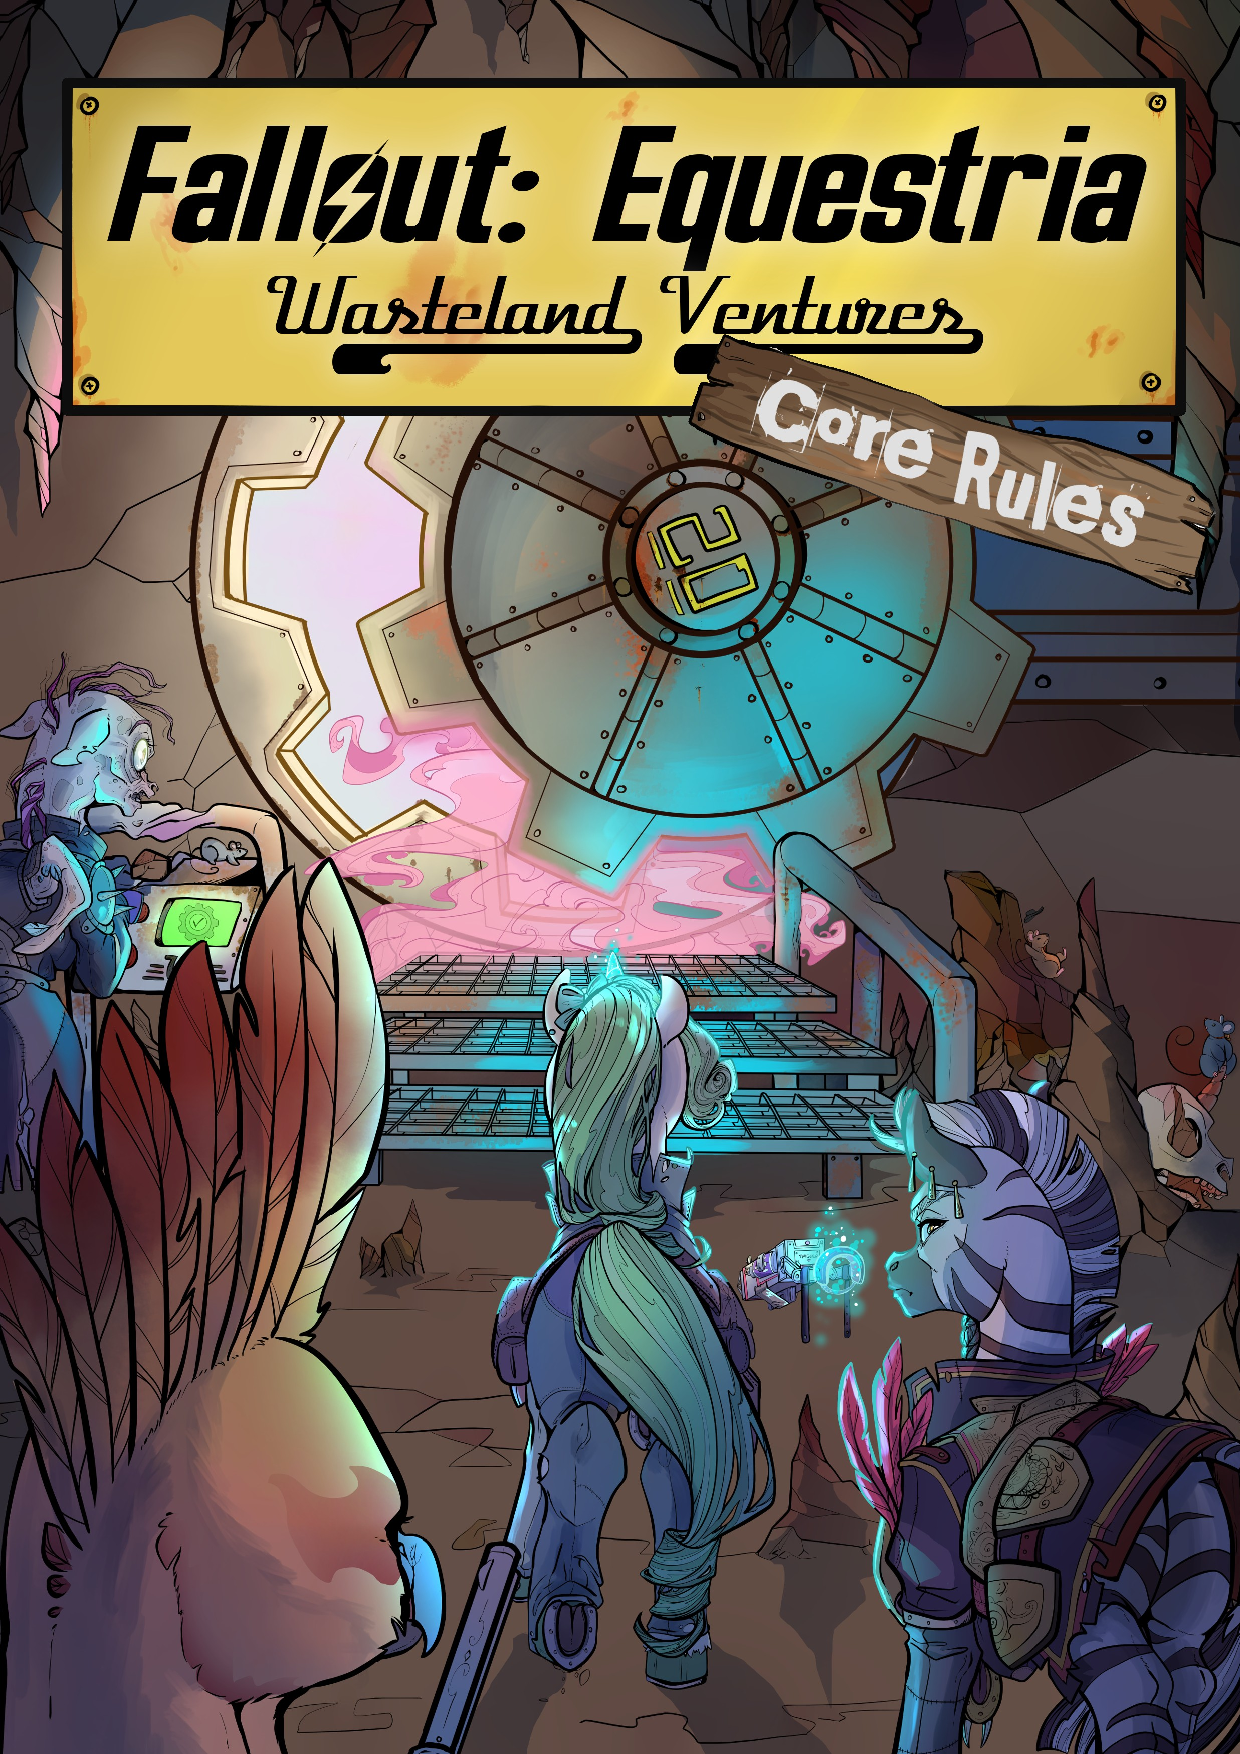
\includepdf[pages={1}]{WORD/COVER-CORE.pdf}	
	\onecolumn	
	\setcounter{page}{1}
	\begin{center}
		Compiled by Waak, Kireanikin, LaPa, Miksu \& SourCherry
		
		10 AP rule basis by Yondalor
		
		Token HP \& Status rule bases by LZ
		
		\bigskip		
		\textbf{Playtesting and Advice:} LZ, Moonlight, Mittens, Kittyfluff, Ray\_Lionheart, f1r3w4rr10r, Tierney Kelly, Eden, Kendallkun, Pesian, Raven, dumbhat, GODOG, Borealis
		
		\bigskip
		\textbf{Cover and Graphics:} SourCherry
		
		\bigskip
		\textbf{Layout:} Waak
		
		\bigskip
		\emph{	Special thanks to:}
		
		\emph{	Kkat - for the fanfiction that sprouted a community}
			
		\emph{	Sunrise - for the original ruleset where all started}
	\end{center}
	
	\vfill
	
	\begin{center}
		\textbf{Version 1.4}
		
		\emph{Last compiled on \thedate}
        
        \emph{\textbf{Contact:} wasteland-ventures@googlegroups.com}
	\end{center}	

	\begin{figure*}[bp]
		\centering
		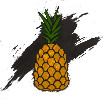
\includegraphics[width=3cm]{Art/ISA_Logo}
		\label{fig:isalogo}
	\end{figure*}

	\twocolumn
	\tableofcontents
	\chapter{Introduction}
	\section*{Beginning}
	\begin{quote}
		\emph{War. War never changes.}
	\end{quote}	
	\noindent
	The chaos of the crumbling world, where no one is or ever will be correct, only but a dream of a once proud, colorful land remains. Here the strong and the determined strife with the law of the Wasteland, and the weak are trampled by those who only see their own twisted needs. All in the world of pastel colored equines and griffons.
	
	\section*{Lore}
	The world of \emph{Fallout: Equestria} begins with a long, arduous war between ponies of Equestria and zebras of Roam over resources. What started out as little more than miscommunication had rapidly developed into a lethal stalemate, where even the most well-intended minds erred.
	
	In this war-torn era, Equestria saw its ruler, Princess Celestia, abdicate her rule to her sister: Princess Luna. She was aided by six heroic mares who would go forth and create Ministries to try and control different aspects of the war-riddled Equestria and bring stability to their citizens.
	
	Sadly, these Ministries would prove to be the undoing of even the most well-intended pony. The war twisted good intentions to foalish naivety, loyalty to secrecy, and trust to treachery. In time, war-torn Equestria saw the rise to weaponry unlike ever before; guns, both ballistic and magical, replaced ceremonial spears and swords.
	
	During the war, new industries arose to cater the needs of the state. One such newcomer - Stable-Tec - went on and created Stables, underground shelters to house a portion of the Equestrian population. However, many of these Stables were also built with social experiments in mind; testing to see if ponies would be able to thrive and coexist peacefully, though many of them failed one way or another.
	
	Eventually the war did come to an end, an apocalyptic one. As the balefire bombs ravaged the land, and those few ponies that had been selected to enter the Stables fled underground, many ponies, griffons and zebra alike perished aboveground. The pegasi retreated behind a cloud cover to stay shielded from the magical radiation. The Equestrian Wasteland was born.
	
	During the next 200 years, magical residue reformed the war-torn land. Damaged buildings would eventually crumble, with only the most prestigious monuments standing. Wild-life, both flora and fauna, mutated into beasts from the greatest of nightmares. Parts of the world would forevermore stay lifeless, while others would bloom in wondrous forms.
	
	Small settlements would eventually form from the survivors and redevelop society in ways they knew of; some trying to work together with mutual, equal trust, while others formed strict dictatorships. Few tried creating utopias of various beliefs, and some fell into utter chaos altogether, creating warring parties of raiders with nary a place to call home. Even some of the Stables would open, greeting the land they might have been oblivious to, with both great fear and absolute arrogance alike.
	
	As the lush, colorful land has mostly turned dry and grim, with great beasts roaming around among other numerous threats, the struggle for food, water, shelter, and all the desires of one's heart is ever present. It is this struggle, that brings both life and end to great many stories. And while some stories have already been long forgotten, others are just about to begin...
	
	\section*{Game}
	\subsection*{Gameplay}
	\noindent
	The classic Pen-and-Paper game in the world of \emph{Fallout Equestria}, a fusion of \emph{Fallout}\textsuperscript{TM} and \emph{My Little Pony}\textsuperscript{TM}. This unpredictable world is contested with just as unpredictable dice and imagination.
	
	Most commonly played as a group, the game can be enjoyed as a short single session experience, or as a long-lasting campaign of multiple sessions, with or without impressive stories to journey through.
	Gameplay is divided into three equal parts: roleplaying, exploration, and combat.
	
	\subsection*{Character}
	\begin{quote}
		\emph{We are not born a monster, but become one through our actions. We do not choose to whom we are born, where we are born, nor when we are born. Only thing that matters, is how we proceed with what we are given...}
	\end{quote}
	
	Players control characters with freedom of thought. They can have personalities different to the player: being wondrous saints, naive rebels, striving business tycoons, or sadistic pillagers, committing both heroics and crimes, and affect the world and story around them. They have backgrounds, experiences that mold their personality, with causes and goals they aim for.
	
	Characters interact with the world, the NPCs they encounter during their journey, and other players with the use of both their stats (attributes and skills) and by describing their actions as the player, not completely limited by stats and numbers. However, stats describe the concept of core character being played, making it rather important trying to act how the character would act, not how the player herself would act. It is part of the immersion of the game, that is being sought after.
	
	\subsection*{Gamemaster}
	The Gamemaster (GM) is the person leading and providing the game. Where rules give the framework of a building, the GM decorates it inside out, and players then interact with it how they see fit.
	
	GM creates the game world, handling the locations, events, quests, NPC's and creatures. She upholds the rules, while is inclined to focus foremost on the enjoyment and excitement of her players.
	
   
    
	\subsection*{World}
	Where Fallout and other pop culture references imagine a nuclear holocaust tearing the world apart, in Fallout Equestria, an uncontrolled magical warfare of Megaspells tore the world apart, creating Equestrian Wasteland. A recovering world molded by magical residue, turned into hostile and savage environment, with skirmishes over resources, struggles against monsters and beasts, and ponies hoping to maintain civilizations and order with knowledge from 200 years before.
	
	The world is where exploration takes place. While most of the old world is lost, few monuments and famed locations still stand tall and prospering in hopes of better tomorrow. And the most sought-after places are those few untouched by the war.
	
	\subsection*{Combat}
	Third section of the gameplay is to overcome character' adversaries when words are not enough. Combat is fought with variety of styles, be they guns from afar, kicks at close and personal, baseball bats and grenades, even magic of varying sort.
	
	Combat is turn-based, every player having their own turn to act accordingly. Combat has variables that change its flow from easy to difficult, like how far opponents are. Part of the combat is to think how to overcome these difficulties.
	
	\subsection*{Meta-Gaming}
	The term used to describe use of knowledge that the players have but characters do not. Such knowledge includes character statistics, other character backgrounds, and information on monster statistics and behaviour learned outside the game. Meta-gaming is considered immersion breaking, and should be left out of roleplaying games.
    
    \begin{figure*}[t]
		\centering
		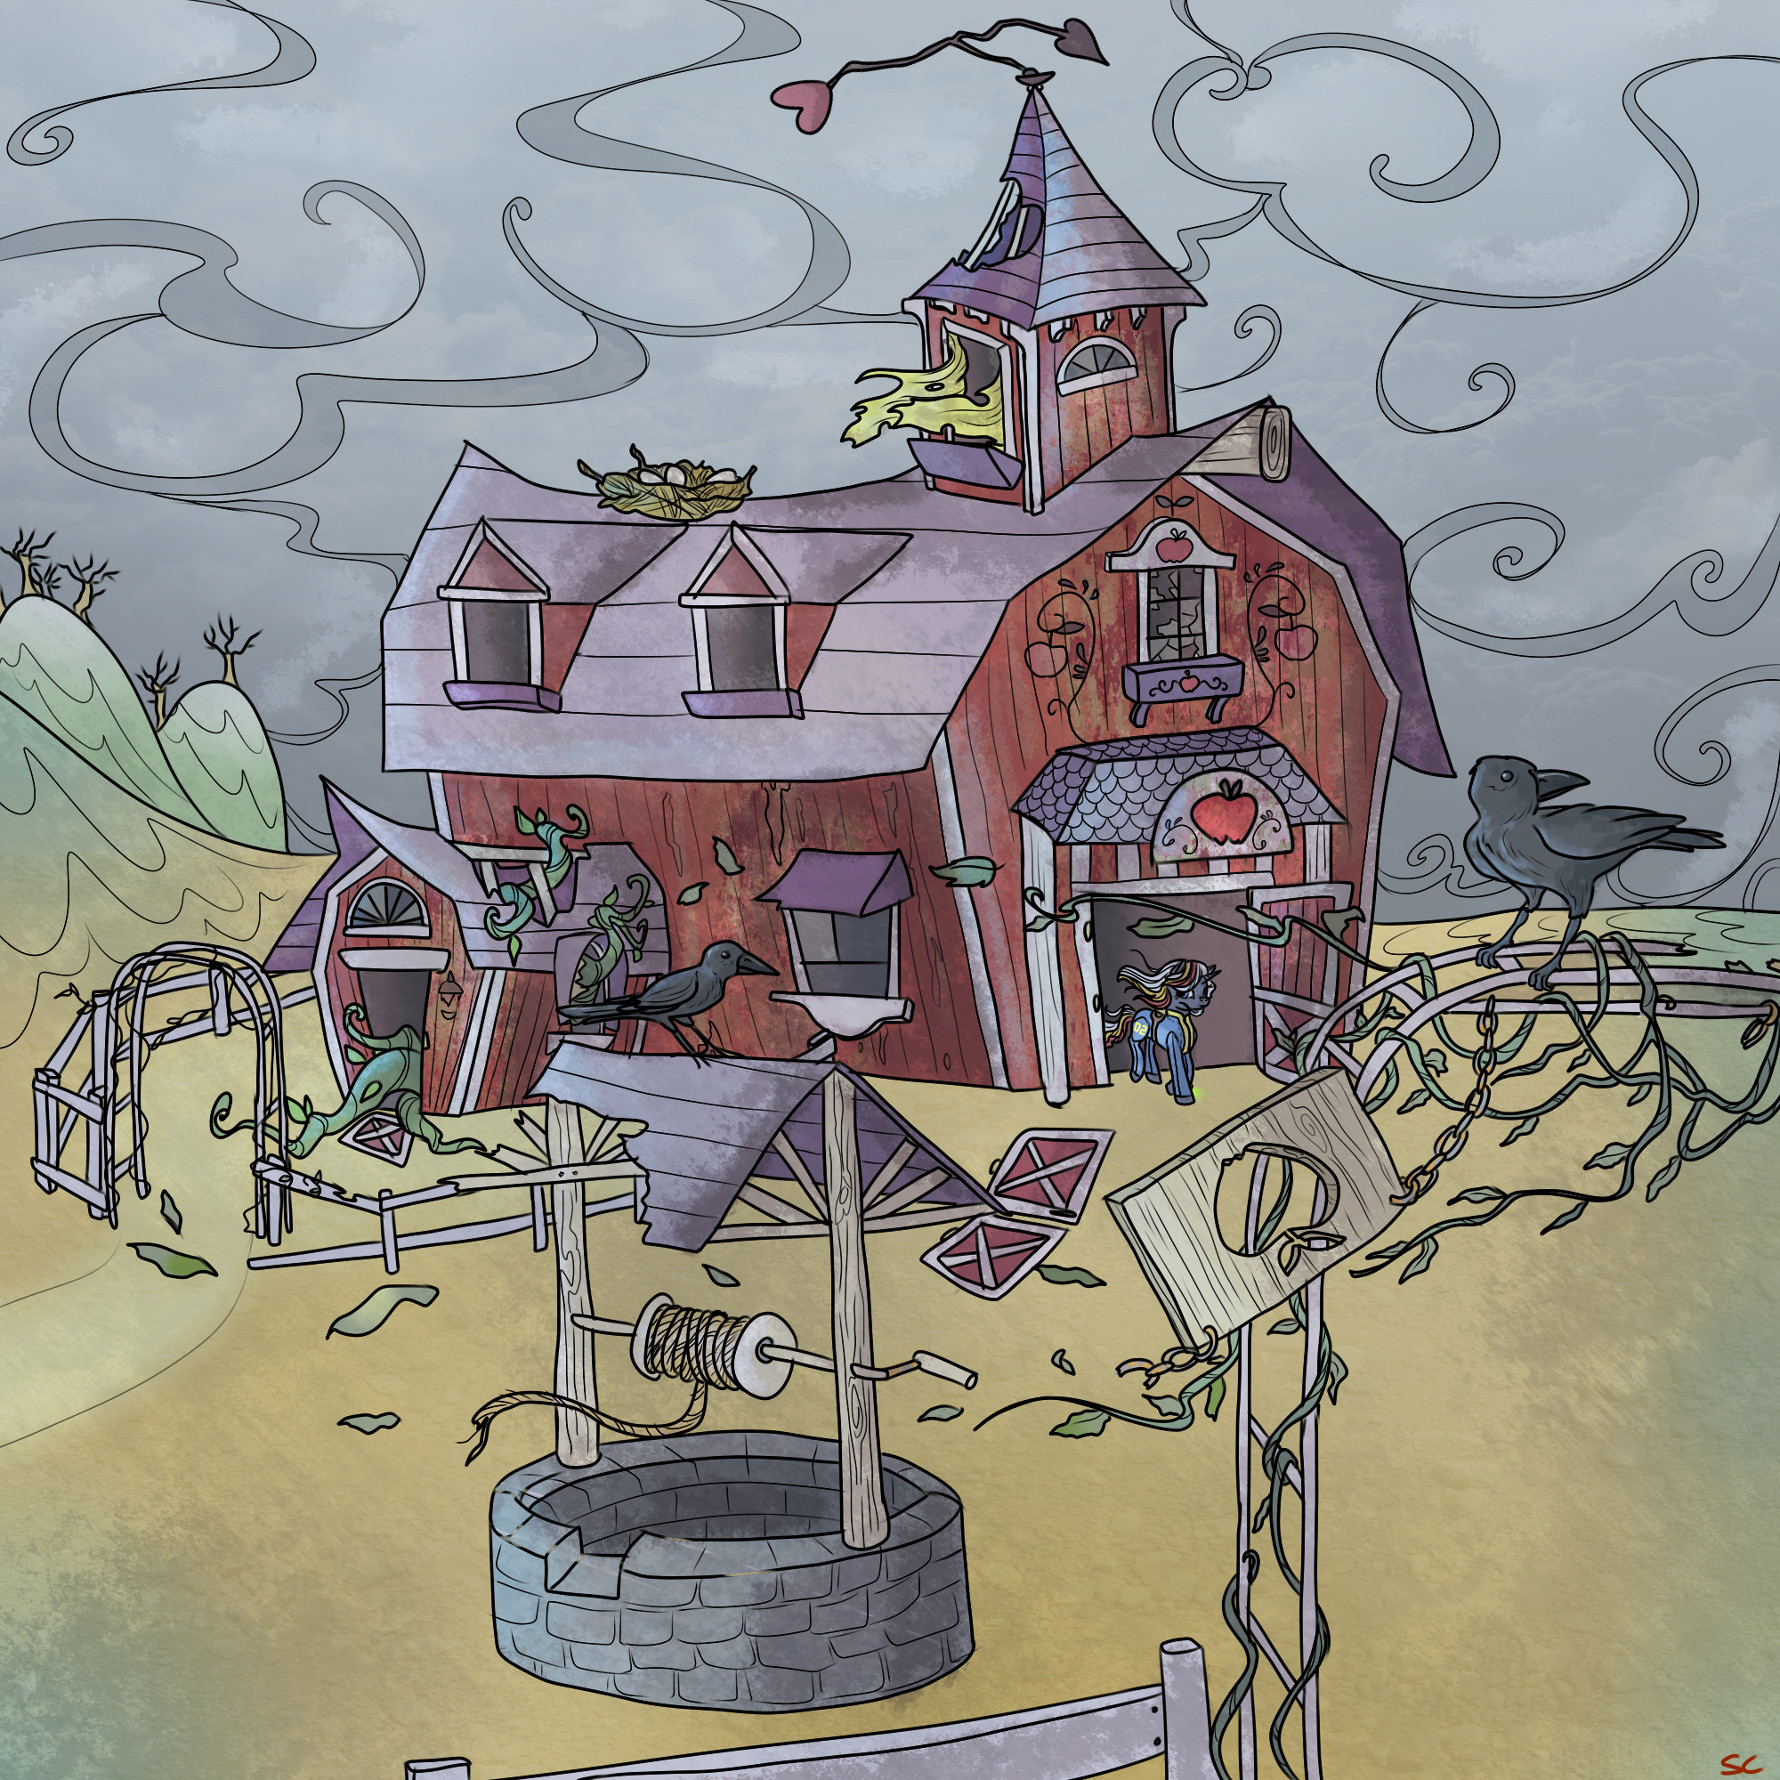
\includegraphics[width=140mm]{Art/AJ_barn}
	\end{figure*}
	
	\chapter{Characters}
	\noindent
	Every story starts with a character - which often are more than just notes and numbers on a paper. This chapter holds the materials you need to create the baseline of your character, while you bring life to it with your roleplaying and imagination.
	
	This rulebook comes with a Character Sheet where you can record the details of your creation.
	
	
	\section*{Creation Process}
	\addcontentsline{toc}{section}{Creation Process}
	When you begin to create your character, you should first decide what kind of a person this character should be; an agile sharpshooter or the slow but deadly stallion with a Super Sledge? Maybe the character is the face of the group, talking their way out of trouble. Once the character concept is done, you can start to determine the details; race, stats, gear and so on.
	
	\subsection*{1. Race}
	Most common races to wander the Equestrian Wastes are of equine descent - these are earth ponies, pegasi, unicorns, and (to some extent) zebras. Griffons are also a playable race in this game. Ghoulified -corpselike mutations- variants of the aforementioned races exists, as well as an array of other races that are up to GM's discretion to allow for play. A list of ``core races'' is provided under Chapter 2: Characters - Races on page 18.
	
	\subsection*{2. SPECIAL}
	At character creation, all characters have 40 points to distribute between 7 SPECIAL attributes - Strength, Perception, Endurance, Charisma, Intelligence, Agility, Luck. The minimum and maximum in each attribute is 1 and 10, respectively. The higher your attribute is, the better! A complete description of the attributes is provided under Chapter 2: Characters - SPECIAL.
	
	\subsection*{3. Secondary Statistics}
	A multitude of secondary statistics are derived from the primary SPECIAL attributes - these further establish your character and provide some key stats in and out of combat. Unless modified with Traits and/or Perks, most of these statistics do not change during gameplay. Most important secondary statistics to note are the following:
	\\
	\begin{compactitem}
		\item 	Hit Points (HP) 
		\item 	Action Points (AP)
		\item 	Carry Weight
		\item 	Healing Rate
		\item	Resistances
		\item 	Critical Success And Failure Thresholds
	\end{compactitem}
	\medskip
	A complete list of secondary statistics and how they are calculated is provided under Chapter 2: Characters - Derived Statistics.
	
	\subsection*{4. Skills}
	Skills are the learned abilities your character has gathered in their life - like knowledge in utilizing guns is shown through Firearms, while computer knowledge and hacking prowess is determined through Science.
	
	Skill values normally range between 1 to 85 - though there are methods to raise a skill above 85, no skill can be raised above 100.
	
	All characters can choose three skills to ``tag''- these tagged skills represent where your character has specialized herself before beginning their adventure and start with an extra 20 skill points. 
	
	A complete list of skills, their initial calculation and associated descriptions is provided under Chapter 2: Characters - Skills.
	
	\subsection*{5. Traits}
	Something else can make your character special than their... well, SPECIAL stats. It's their flaws and special powers that make them more interesting. Characters can take up to two traits with their associated benefits and hindrances. Note that a few of them requires GM's approval - you'll find the full list of traits under Chapter 2: Characters - Traits.
	
	\subsection*{6. Virtue, Karma \& Special Talent}
	A character's \textbf{virtue} is the one good trait that helps them weather the wasteland's worst storms of the character's life and from where they draw power from when faced with difficult situations. This is purely for roleplaying purposes in order to give the character more depth.
	
	\textbf{Karma} measures how good, neutral or evil a character is. Characters start with +10, 0 or -10 karma. Karma is sensed by others; it shines through the way the character carries themselves, the way they speak and the way they act. Unless you take a perk to mask Karma, NPC's are capable of ``having a hunch'' about your character's true standing, which can change how they act and treat your character.
	
	Negative karma stands for karma gained out of acts that are frowned upon; stealing, senseless killing and backstabbing among others.
	Positive karma is gained by doing good deeds; letting enemies live if given the chance and using more peaceful solutions.
	
	A neutral karma character has their karma stay close to 0. This means most characters with more extreme karma are less affected by the neutral karma character.
	
	Karma influences how NPC's react to the characters. Characters that have high positive karma rarely see eye to eye with characters of negative karma, and vice versa.
	
	\textbf{Special talent} is reserved for characters whose race is of any equine heritage. The special talent is the one thing a character is very good at, making them special. If the character is a pony, they have a cutie mark symbolizing the special talent. If the character is a zebra, they have a glyph that represents this talent.
	
	This special talent has to be related to one of your tagged skills. When using your special talent related skill, you can get a slight bonus of +5 on specific or all actions. This should be discussed with the GM.
	
	\begin{verse}
			\emph{	\textbf{Example:} Emerald Glint has a Cutie Mark of a dismantled mine. The player and GM have decided that this Cutie Mark means that Emerald Glint's special talent is disabling mines and perhaps an occasional time bomb. This means that each time Emerald Glint tries to disable a mine, her Explosives skill gets a +5 bonus.}
	\end{verse}
	
	\subsection*{7. Gear}
	You can't go out into the harsh wasteland and expect to survive without equipping yourself. Gear includes armor, weapons and general survival tools such as food, water, and a saddlebag.
	
	Some settings may provide you with the basic items you need and sometimes you have to purchase all of your gear by yourself.
	
	When equipping armor and clothing, only one of each can be worn on the body simultaneously. However, some clothes cannot be worn with armor.
	Unless otherwise specified by the GM, the standard starting amount is 500 caps at level 1.
	
	Further information on equipment and their statistics can be found under Chapter 3 - Equipment.
	
	\subsection*{8. Background}
	You can do the finishing touches to your character by filling in the name, history and background you deem important for them, making the character more unique. You can ask why your character has decided to go on the adventure provided by your GM. Do not shy from discussing with other players - it is possible the characters know each other from previous encounters and share history.
	
	It is also encouraged, but not necessary, to try and think what kind of fears or dreams your character has, to give them a longer lasting goal and depth. All these details can be written down on the Character Sheet.

	\clearpage
		
	\section*{Races}
	\addcontentsline{toc}{section}{Races}
	The following races are the most common to roam Equestrian wastes, surviving the day-to-day life or going on life-threatening adventures. Most - though not necessarily all - playable races are various kinds of equines, or quadrupeds in all the colors of the rainbow. Ghoul variants of these are made with picking an appropriate Trait Ghoul listed under Traits section in this chapter.
	
	\subsection*{Earth Pony}
	
	\begin{figure}[b]
		\centering
		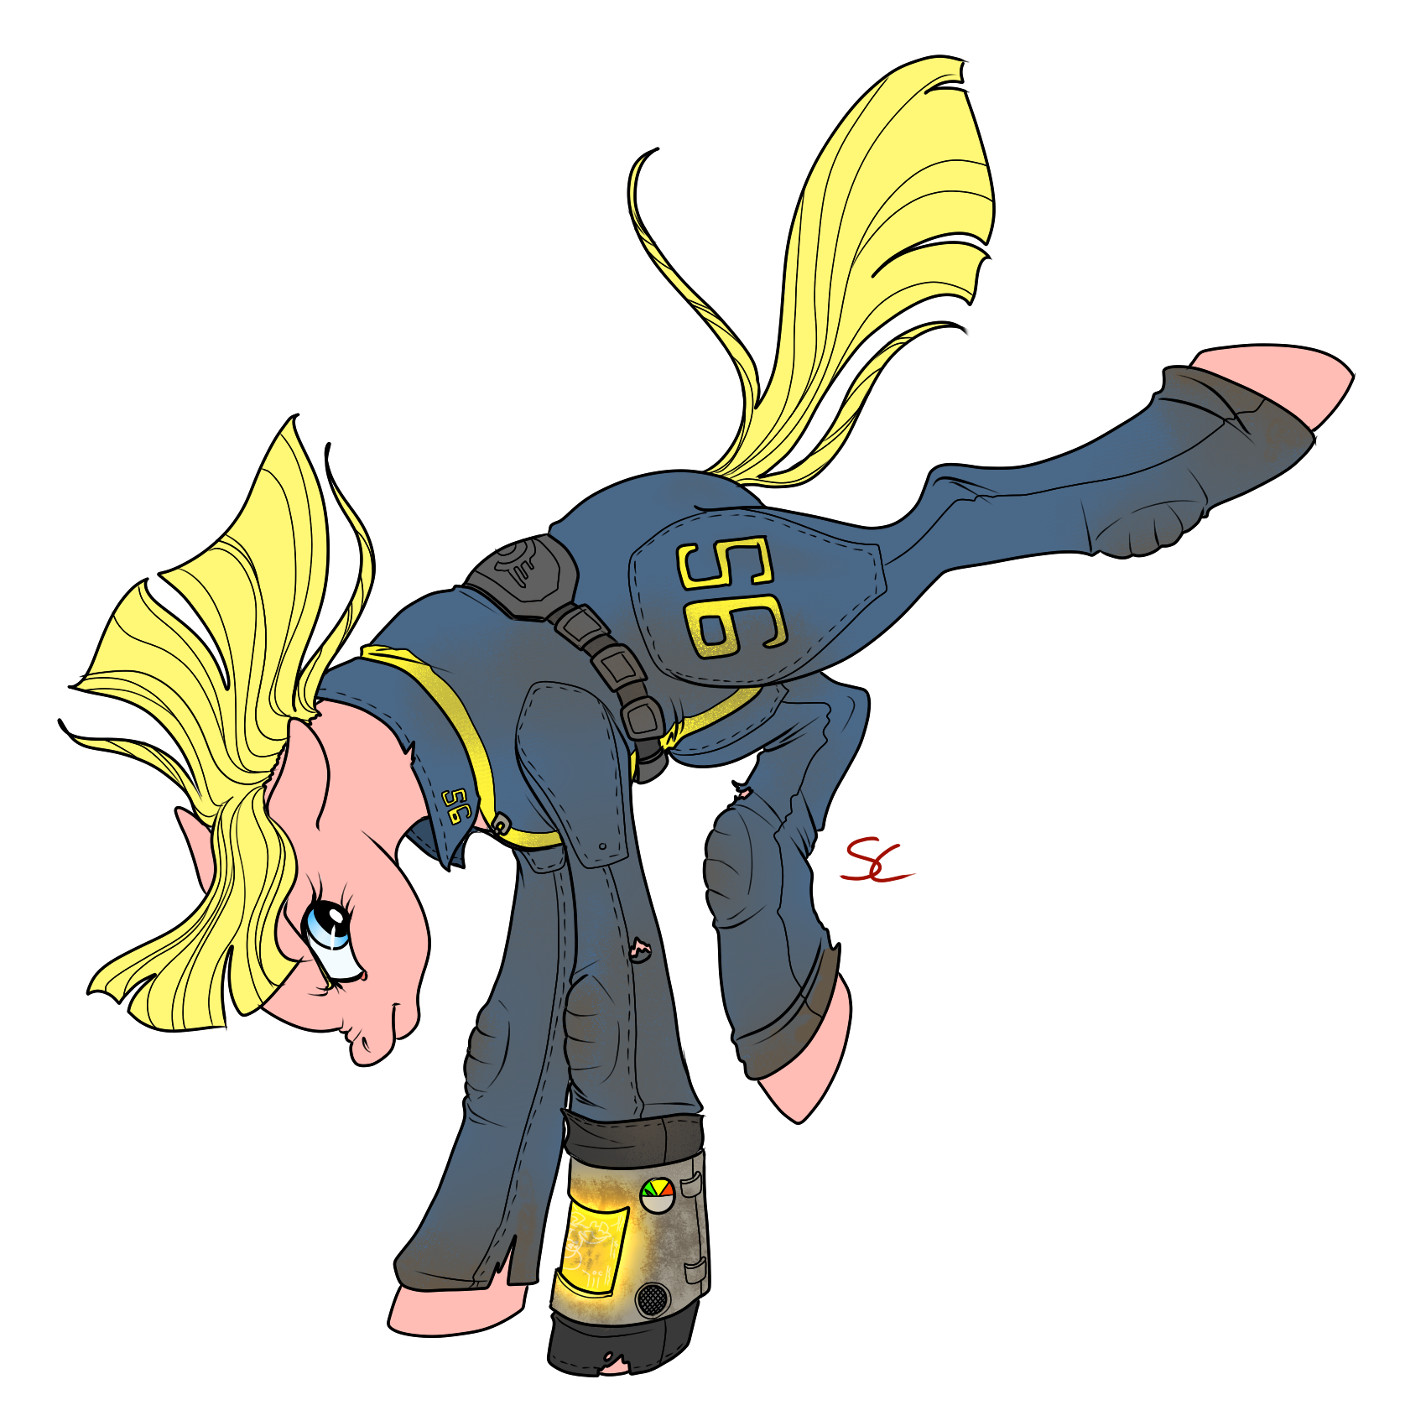
\includegraphics[width=0.8\linewidth]{ART/Races/EP_F}
	\end{figure}
	
	\begin{figure}[b]
		\centering
		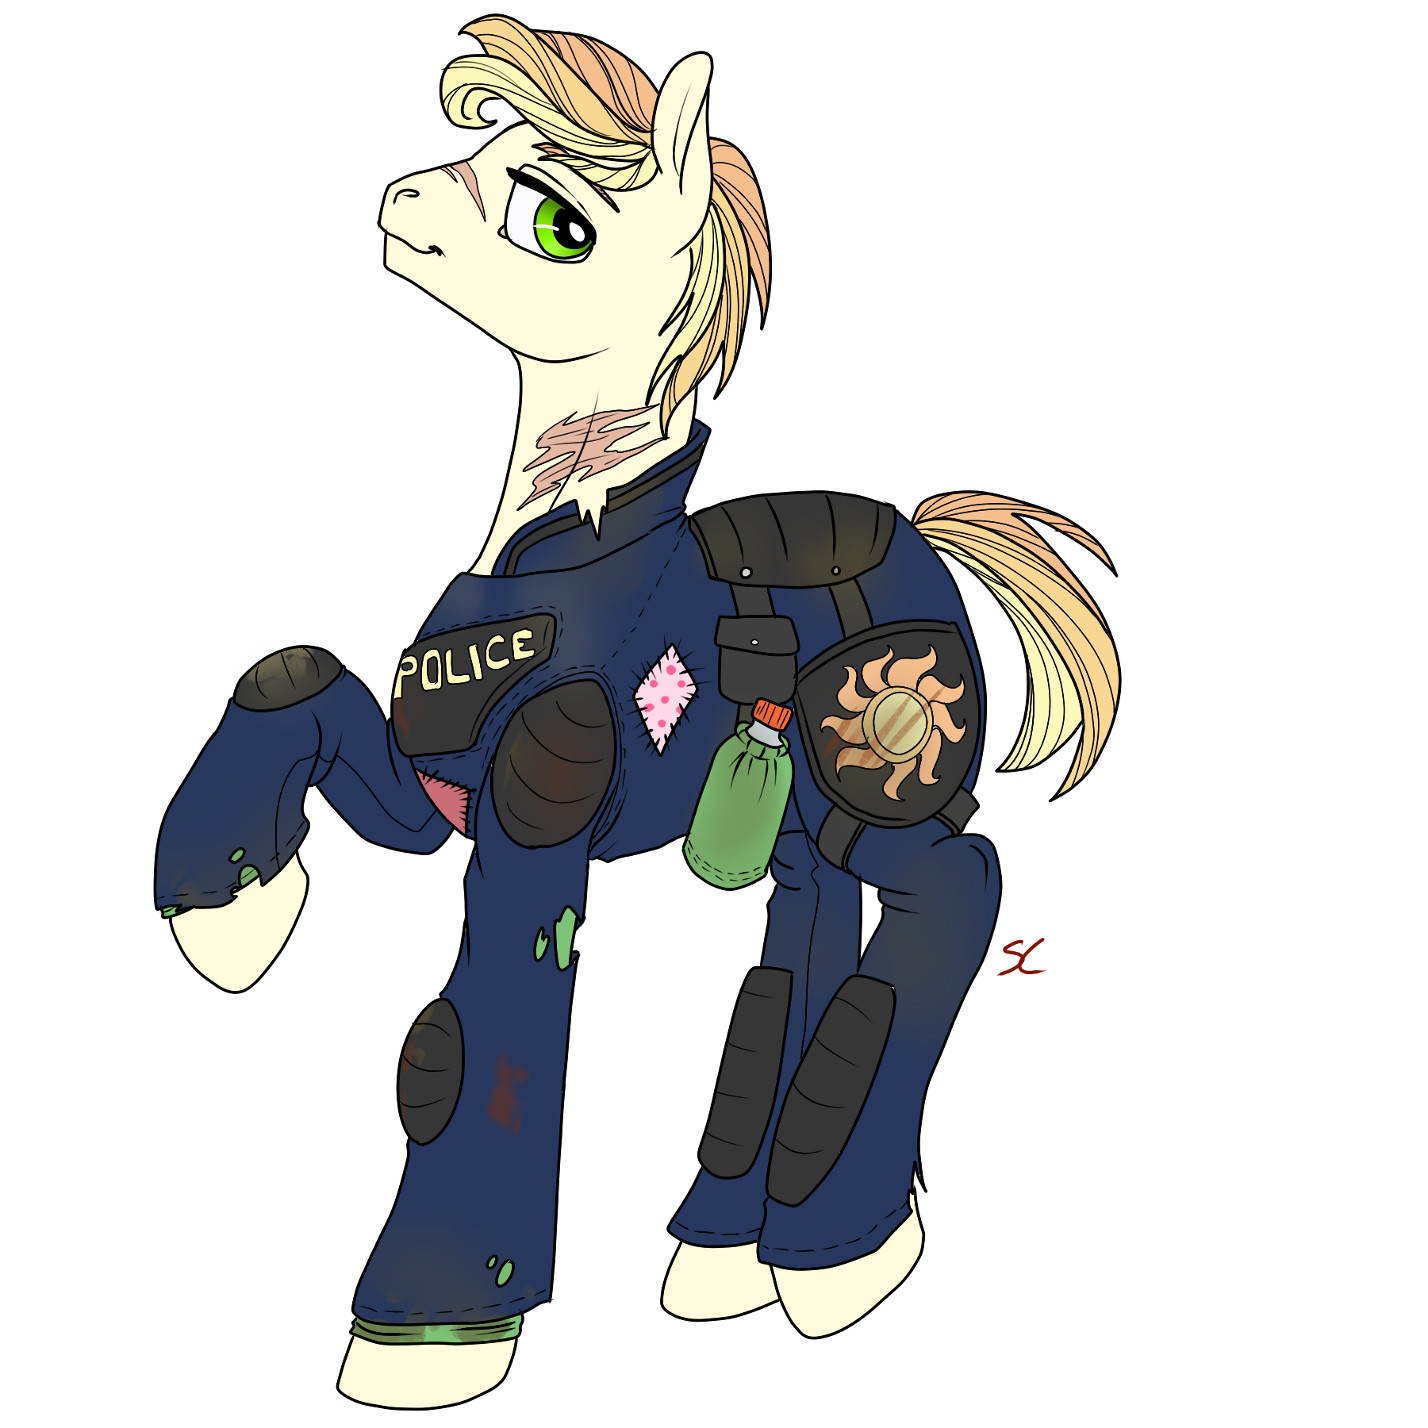
\includegraphics[width=0.8\linewidth]{ART/Races/EP_M}
	\end{figure}
	
	Your basic pony. Four legs, two eyes, mane and tail. Earth ponies have neither wings nor horns. Instead, they are generally stronger, larger, and have more stamina than the other two pony races - having to do everything by hoof or by mouth.
	
	By far the most common race alongside unicorns in the Equestrian Wasteland, as long as only Equestria is accounted for. A common sight in both big and small settlements, earth ponies tend to make their home nearly anywhere, excluding crater sides and the Canterlot Ruins. 
	
	Many of the earth ponies survived either due to their own home-built bomb-shelters, or in the many Stables from which they made their way to the post-apocalyptic Wasteland. Not being ones to lay on their laurels, many earth ponies took to rebuilding settlements or making new ones. One such testament is New Appleloosa, built a stone's throw away from the old one, now overtaken by raiders.
	
	Earth ponies have the following racial abilities:
	\begin{description}
		\item[Cutie Mark:] Earth Ponies have a \textbf{Special Talent}, giving them a +5 to a skill when using their special talent.
		\item[The Hard Way:] At 1st level Earth Ponies may choose a free perk that they qualify for; the perk level requirement can be up to level 4. In addition they ignore 1 STR requirement on Firearms (to a minimum of 1).
		\item[Close to Earth:] Earth ponies may perform Earth pony magic. They can choose 2 spells at 1st level they have the requirements for, and gain a new one every 5 levels after (6th, 11th...).
		\item[Earth Pony Ingenuity:] Earth ponies may invent schematics based on their Special Talent, using the associated Tag Skill for Invention rolls instead of Science.
	\end{description}

	\clearpage
	\subsection*{Pegasus}
	
	\begin{figure}[b]
		\centering
		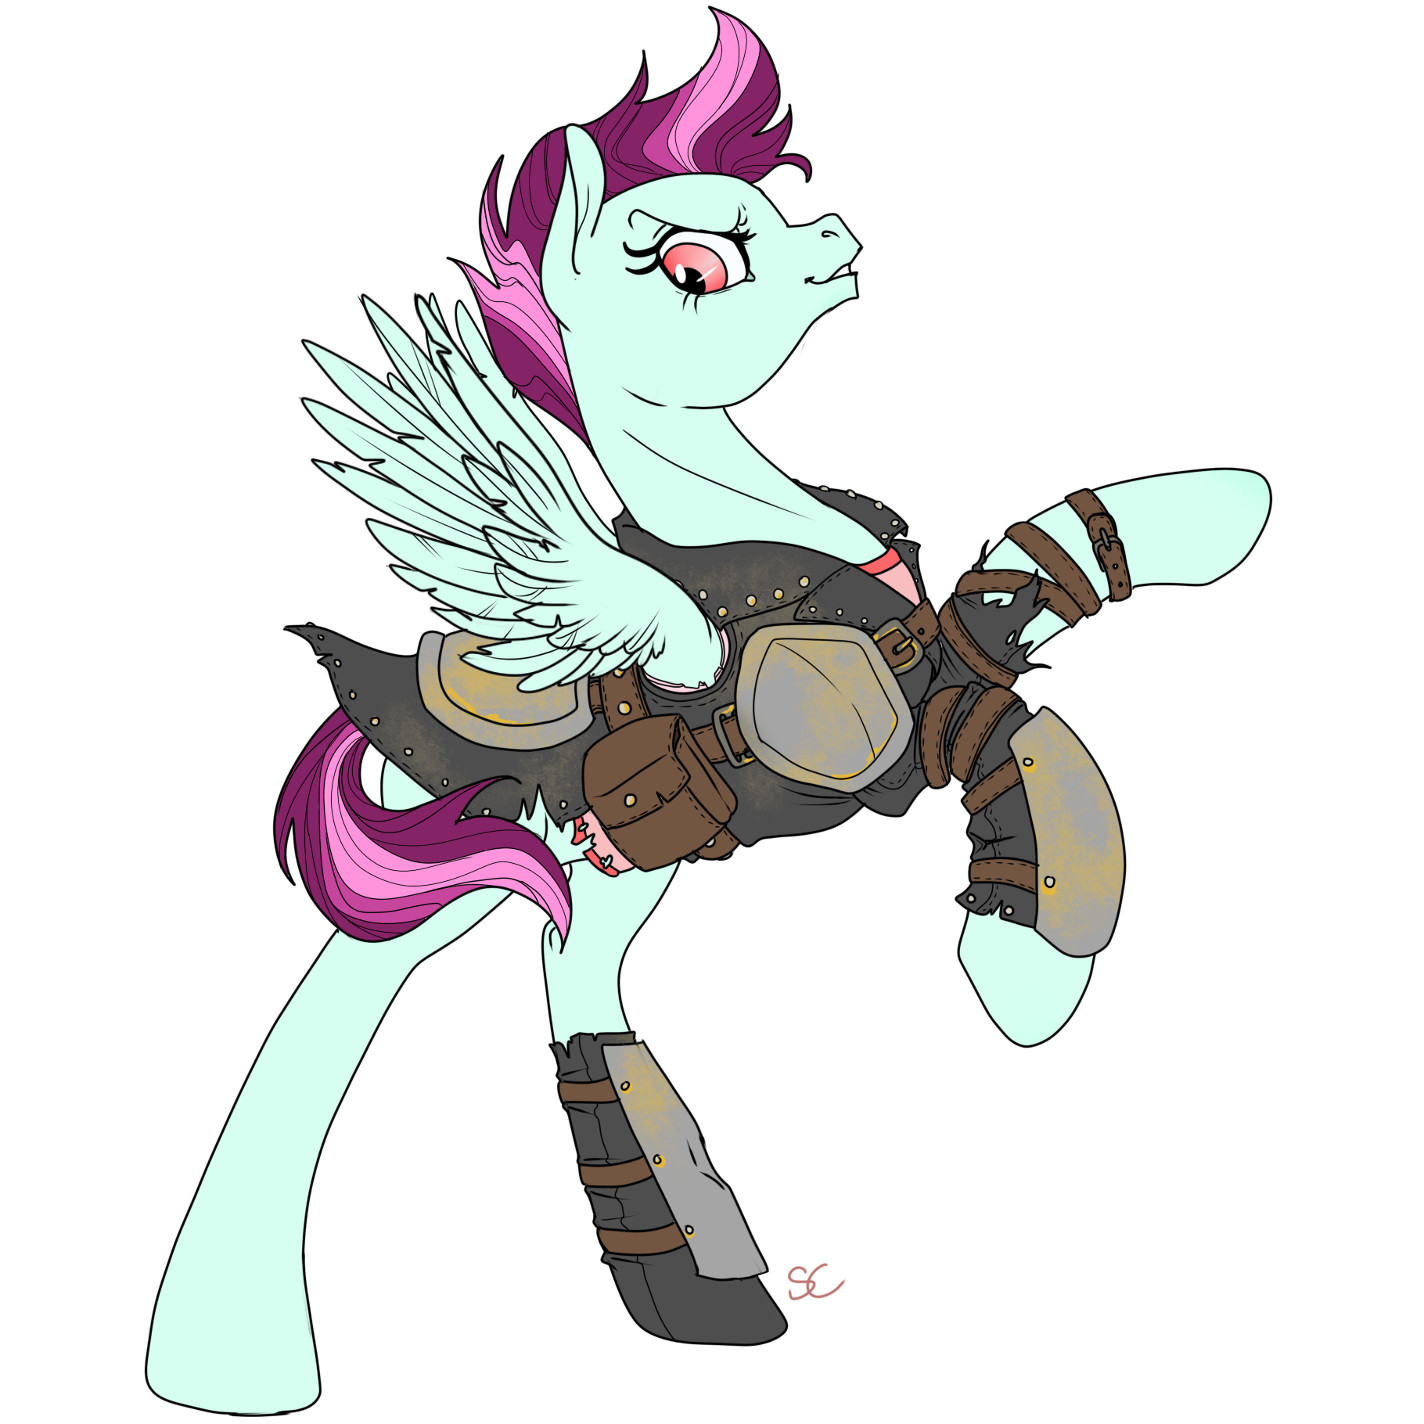
\includegraphics[width=0.8\linewidth]{ART/Races/PEG_F}
	\end{figure}

	\begin{figure}[b]
		\centering
		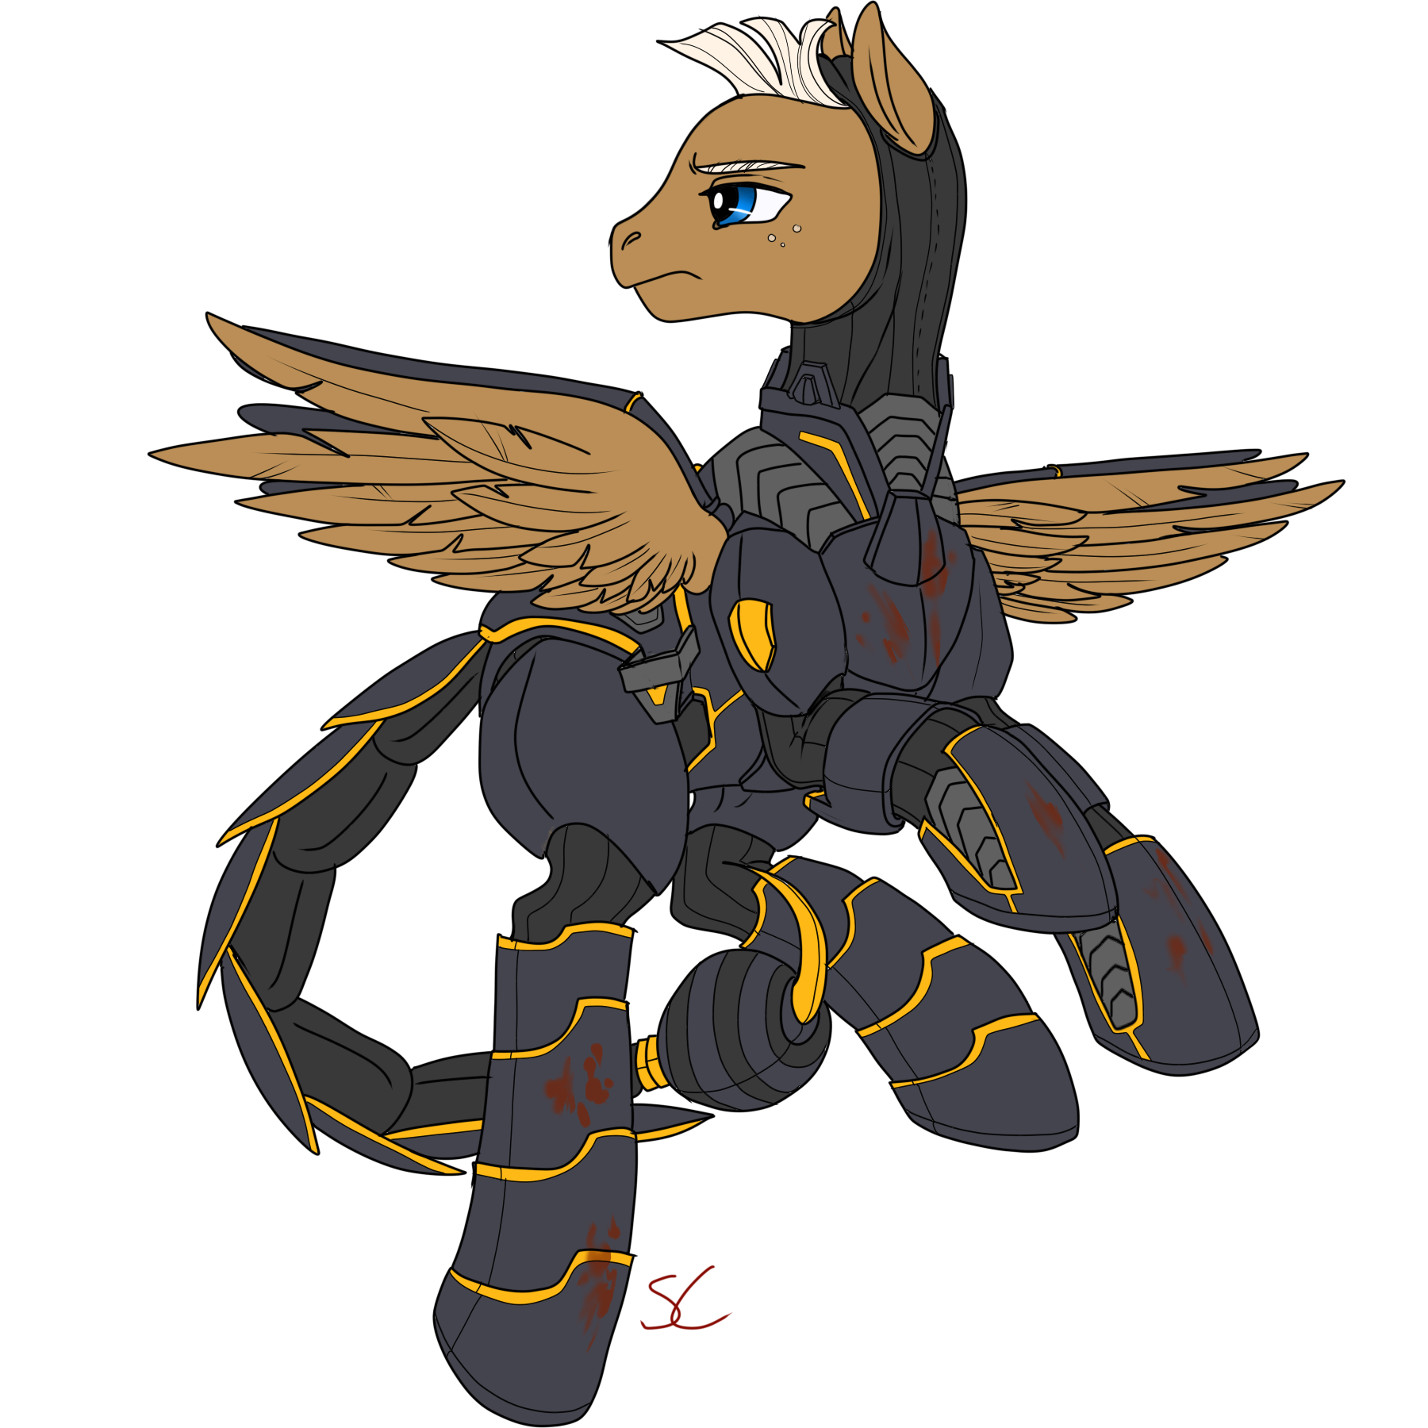
\includegraphics[width=0.8\linewidth]{ART/Races/PEG_M}
	\end{figure}
		
	Pegasi are characterized by the feathered wings that grow above and slightly behind the front legs. Though small in appearance, they allow these ponies to fly. Pegasi are normally associated with control of the weather - they are the only pony able to interact with clouds as if they were tangible, allowing them to disperse clouds for extra sunlight or gather clouds for various forms of precipitation.
	
	During the Balefire attack that destroyed Equestria, the pegasi closed off the sky with a cloud barrier. Due to this, pegasi are a relatively rare sight in the Wasteland. The few that dot the Equestrian Wasteland are either Dashites - traitors to the Grand Pegasus Enclave, a militaristic faction above cloudbarrier - or born from the surviving Stable-dwellers. Some may be a kink in the genetic code, where a pegasus gene suddenly surfaced after generations of laying dormant... Much to the surprise of the parents.
	
	Pegasi have the following racial abilities:
	\begin{description}
		\item[Cutie Mark:] Pegasi have a \textbf{Special Talent}, giving them +5 to a skill when using their special talent.
		\item[Wings of Glory:] Pegasi have wings and can fly. They can increase their flight capabilities by investing in Aerial Maneuvers.
		\item[Wonder Maneuvers:] Pegasi may perform Aerial Maneuvers. They can choose 3 at 1st level they have the requirements for, and gain a new one every 5 levels after (6th, 11th...).
		\item[Quick Recovery:] Pegasi, due to being airborne often, have developed a slight tolerance to shocks and blunt force traumas. They have +1 END when resisting Stun- status effect.
	\end{description}
	
	\clearpage
	\subsection*{Unicorn}
	
	\begin{figure}[b]
		\centering
		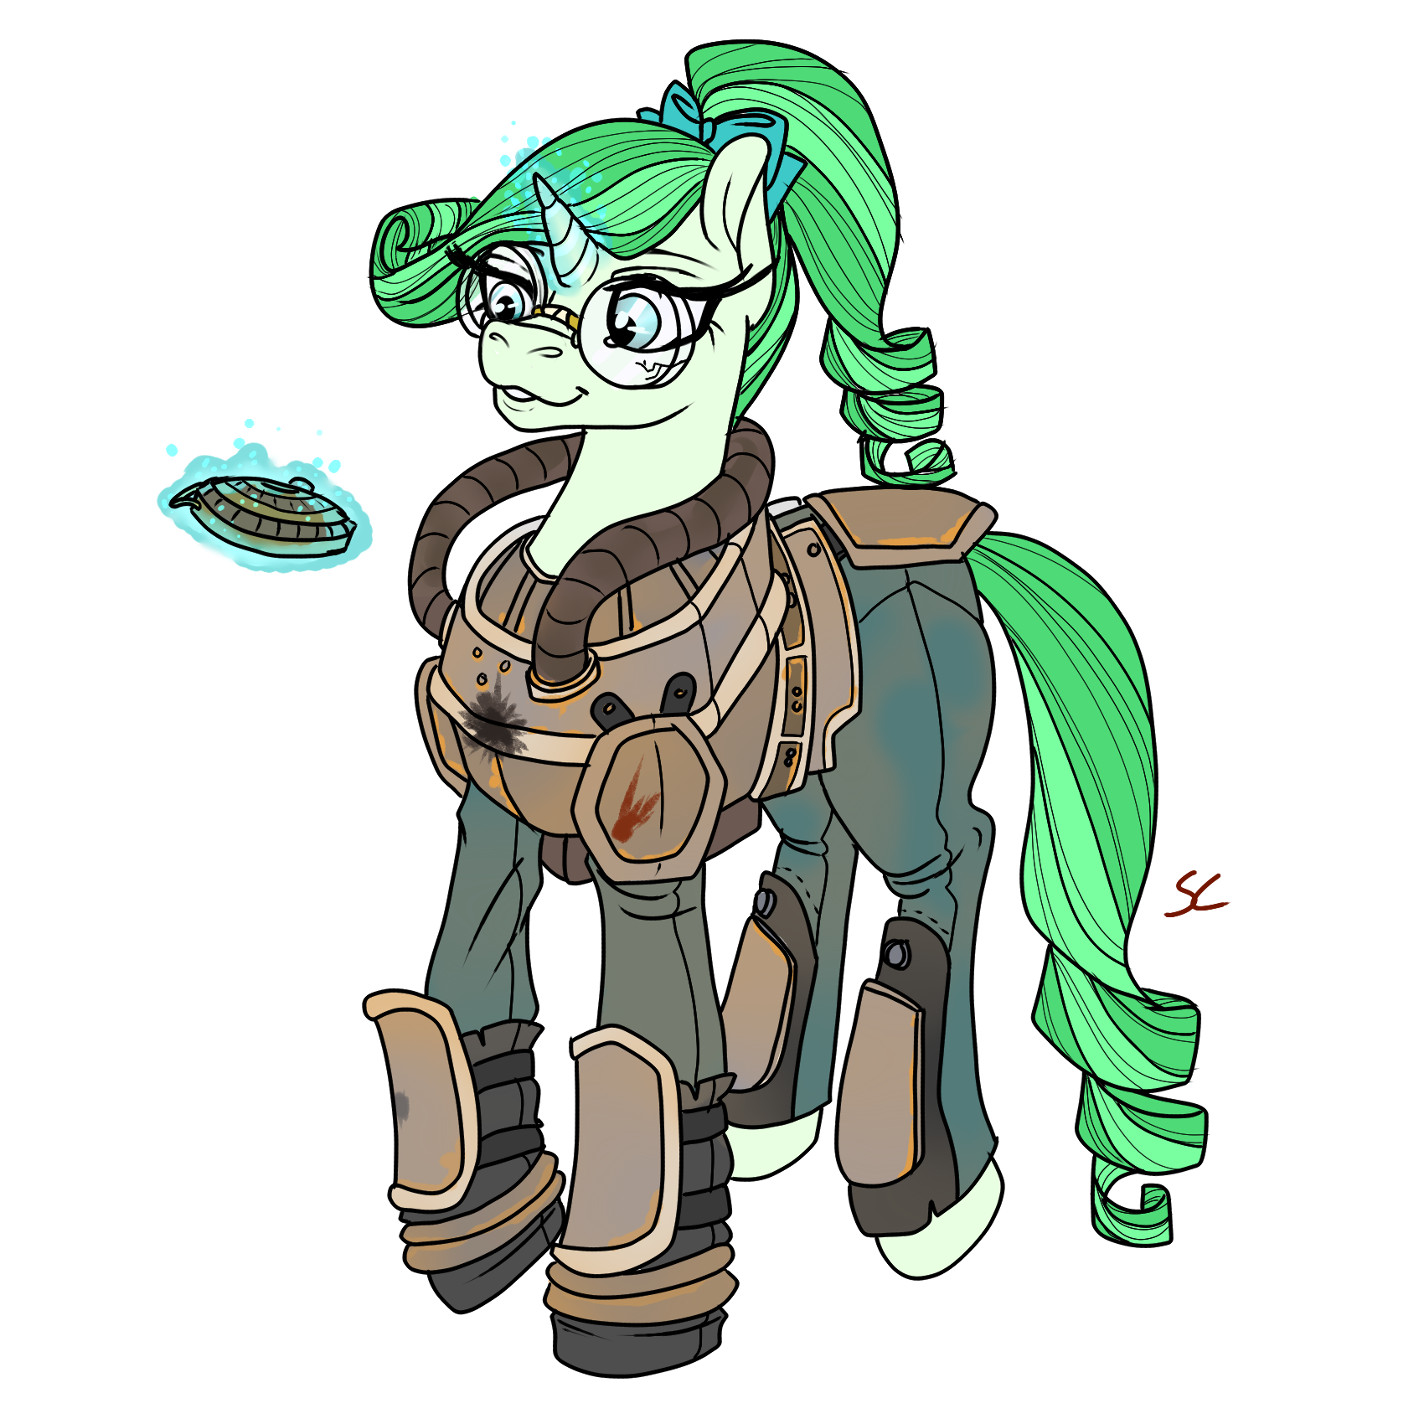
\includegraphics[width=0.8\linewidth]{ART/Races/UNI_F}
	\end{figure} 

	\begin{figure}[b]
		\centering
		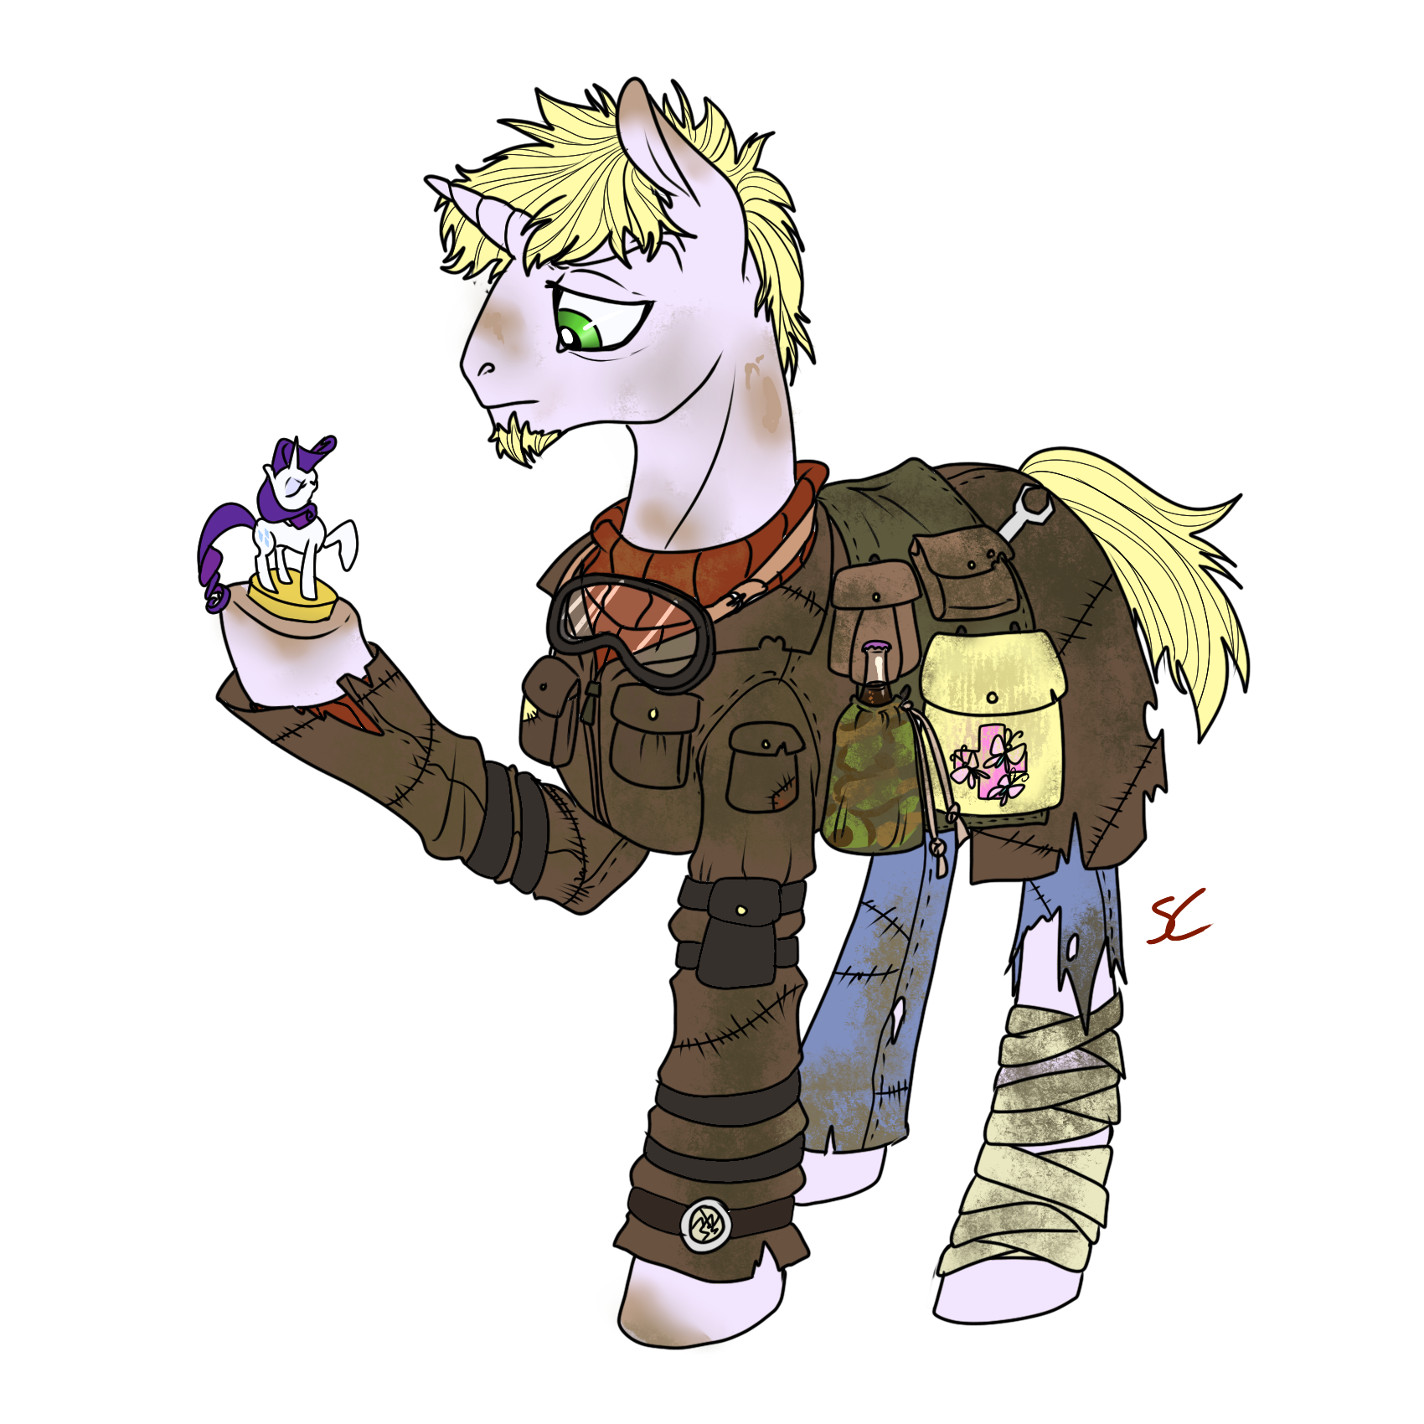
\includegraphics[width=0.8\linewidth]{ART/Races/UNI_M}
	\end{figure}
	
	
	Unicorns stand out among ponies with their ability to wield and manipulate magic. They are identified by a single horn growing from the forehead. The use of magic allows unicorns to perform delicate tasks easily, such as lock picking.
	
	Second most common sight in the Equestrian Wasteland, unicorns tend to take the kind of jobs that magical finesse is better suited for than hooves. Though they might rely a bit on their magic even in most basic of tasks, they have a wide array of spells at their disposal, which makes them handy for many situations and jobs. 
	
	Due to the balefire missiles that decimated Canterlot, the Equestrian capital, unicorns no longer have a place purely of their own. Many of the unicorns alive today are the descendants of Stable dwellers, Stable dwellers themselves or the few lucky ones who found themselves a bomb shelter of their own.
	
	
	Unicorns have the following racial abilities:
	\begin{description}
		\item[Cutie Mark:] Unicorns have a \textbf{Special Talent}, giving them +5 to a skill when using their special talent.
		\item[Death's Offspring:] As the original creators of the weapons that brought the world to ruin, Unicorns are naturally more resistant to the arcane fallout; Their starting Rad Resistance is 10 instead of 5.
		\item[Master of Arcane:] Unicorns may cast spells through their horn. They can choose 3 spells alongside Light and Telekinesis at 1st level, and gain a new one every 5 levels after (6th, 11th...).
	\end{description}
	
	\clearpage
	\subsection*{Griffon}
	
	\begin{figure}[b]
		\centering
		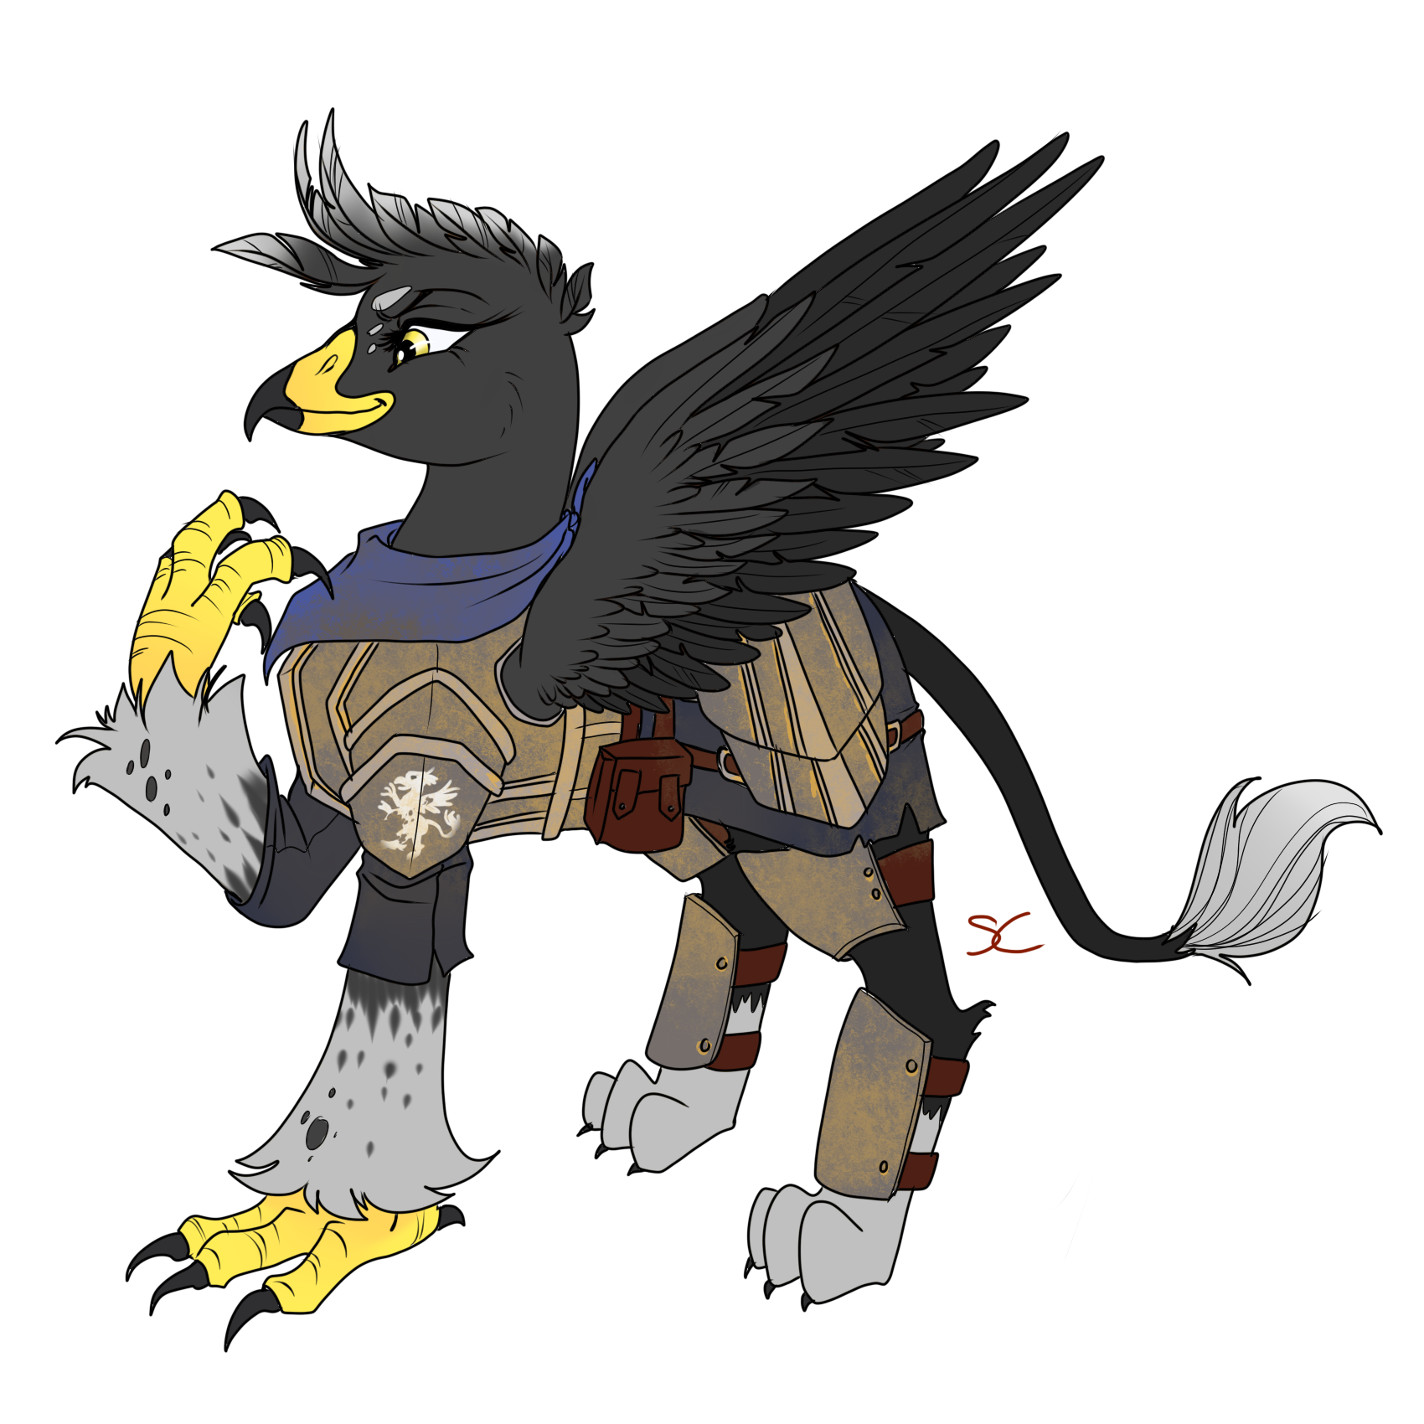
\includegraphics[width=0.8\linewidth]{ART/Races/GRI_F}
	\end{figure}

	\begin{figure}[b]
		\centering
		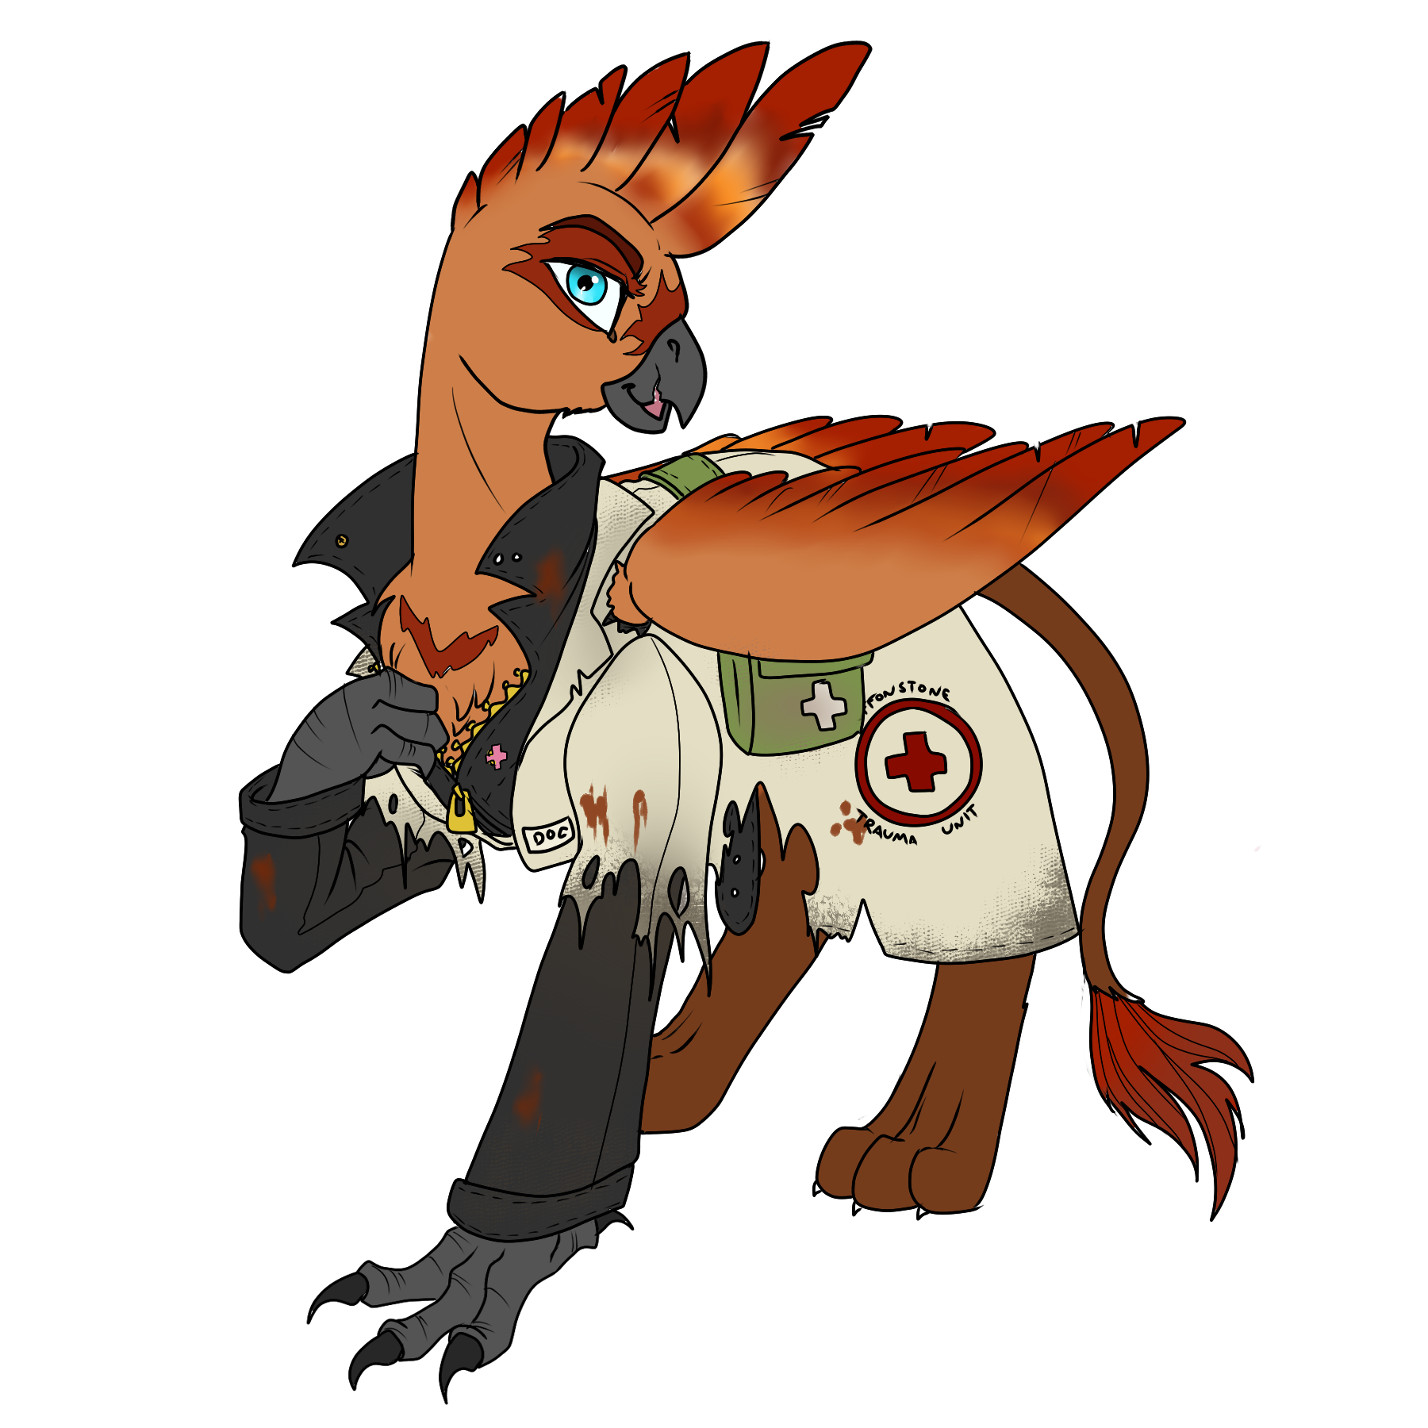
\includegraphics[width=0.8\linewidth]{ART/Races/GRI_M}
	\end{figure}
	
	Griffins, griffons or gryphons - they all mean the same, the amalgamation that is the front of a bird and the behind of a feline creature. Griffons were often employed by the warring sides as mercenaries, a line of profession many still continue to the present day. The collective Talon Company has in it many different groups of griffons, often varied in morality. Much like ponies, they can be of many various colors and various feline species.
	
	Griffons have the following racial abilities:
	\begin{description}
		\item[Stable Wings:] Griffons have wings and can fly. They can increase their flight capabilities by investing in Aerial Maneuvers.
		\item[Talon Maneuvers:] Griffons have a limited ability to perform Aerial Maneuvers. They can choose 2 at 1st level they have the requirements for, and gain a new one every 6 levels after (7th, 13th...).
		\item[Predator:] Griffons possess natural talons, giving them an extra dice to damage when using bare talons as Unarmed weapons.
		\item[Great Beast:] Griffons are visibly larger than ponies, and have heavier builds. All Griffins are considered to be Size Category 1 at start, and they also gain an extra SPECIAL point to invest during character creation.
	\end{description}
	
	\clearpage
	\subsection*{Zebra}
	
	\begin{figure}[b]
		\centering
		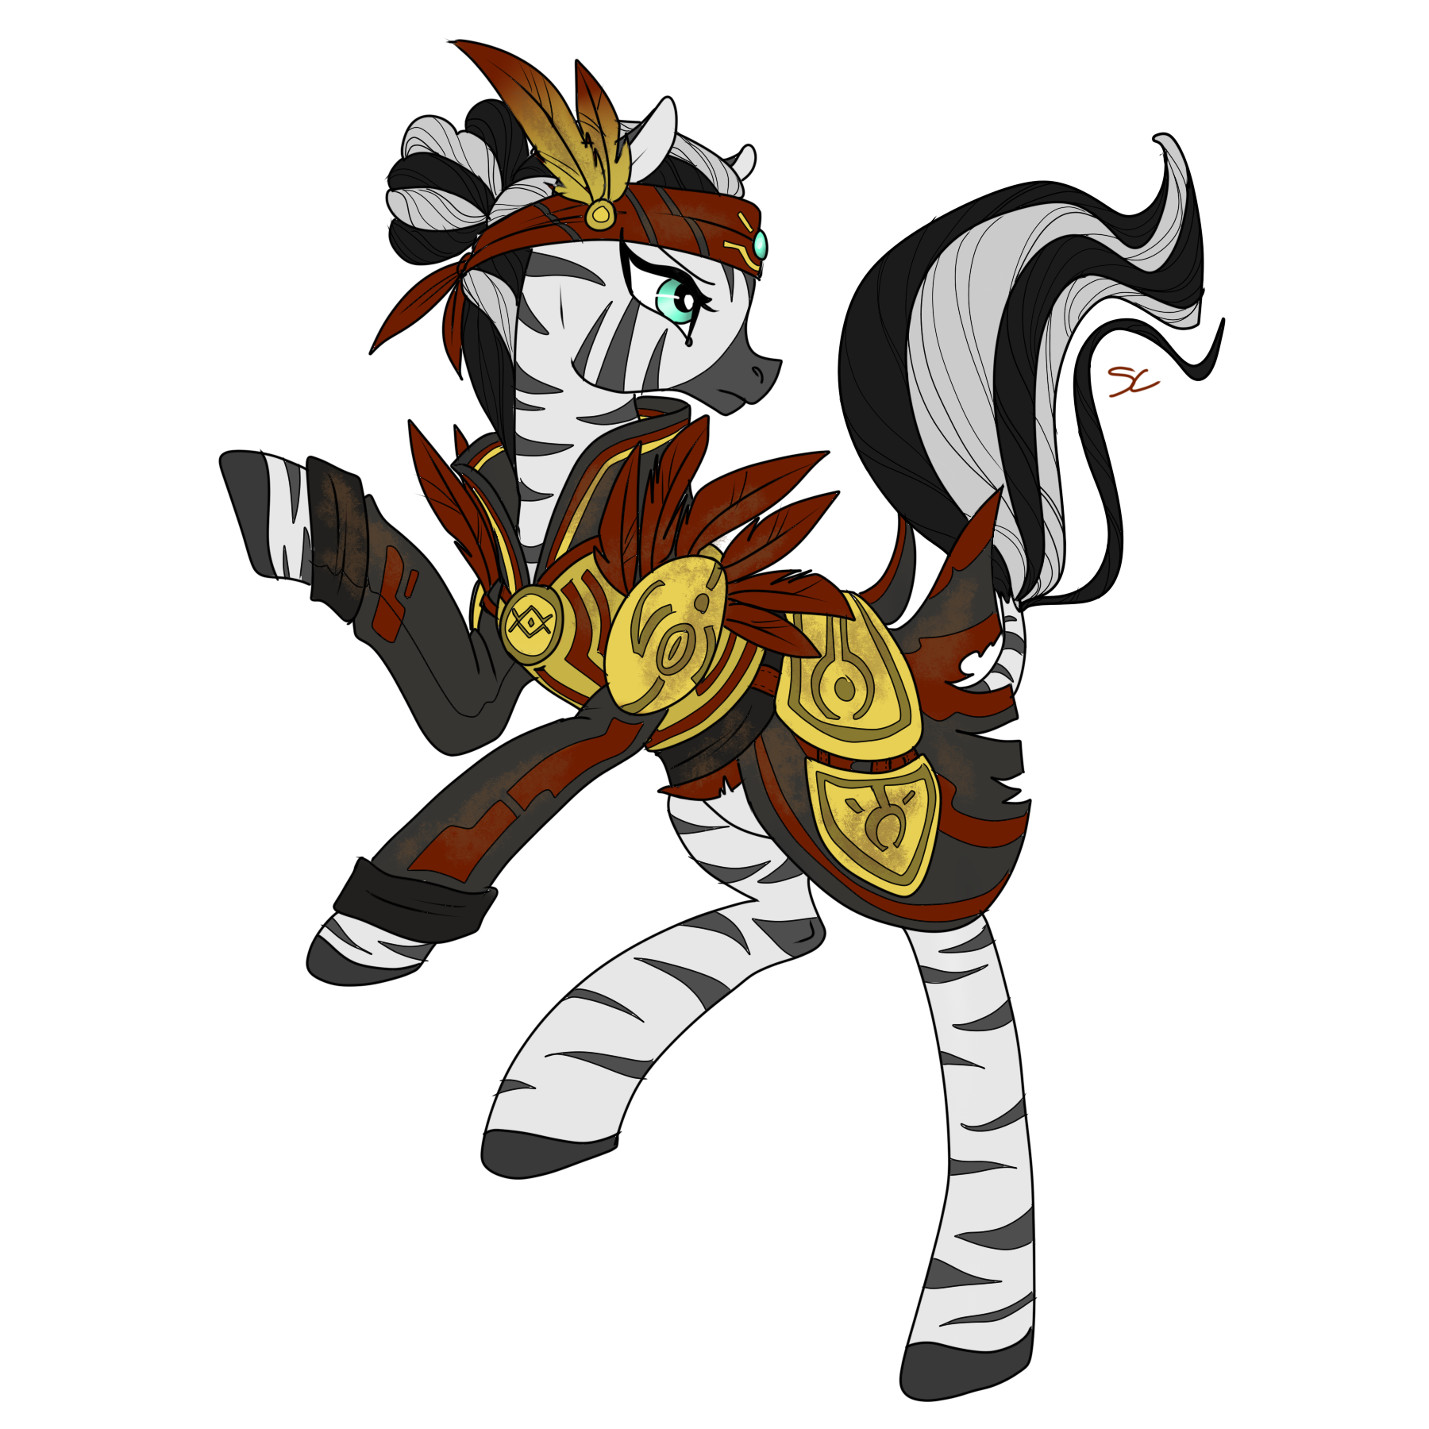
\includegraphics[width=0.8\linewidth]{ART/Races/ZEB_F}
	\end{figure}
	
	\begin{figure}[b]
		\centering
		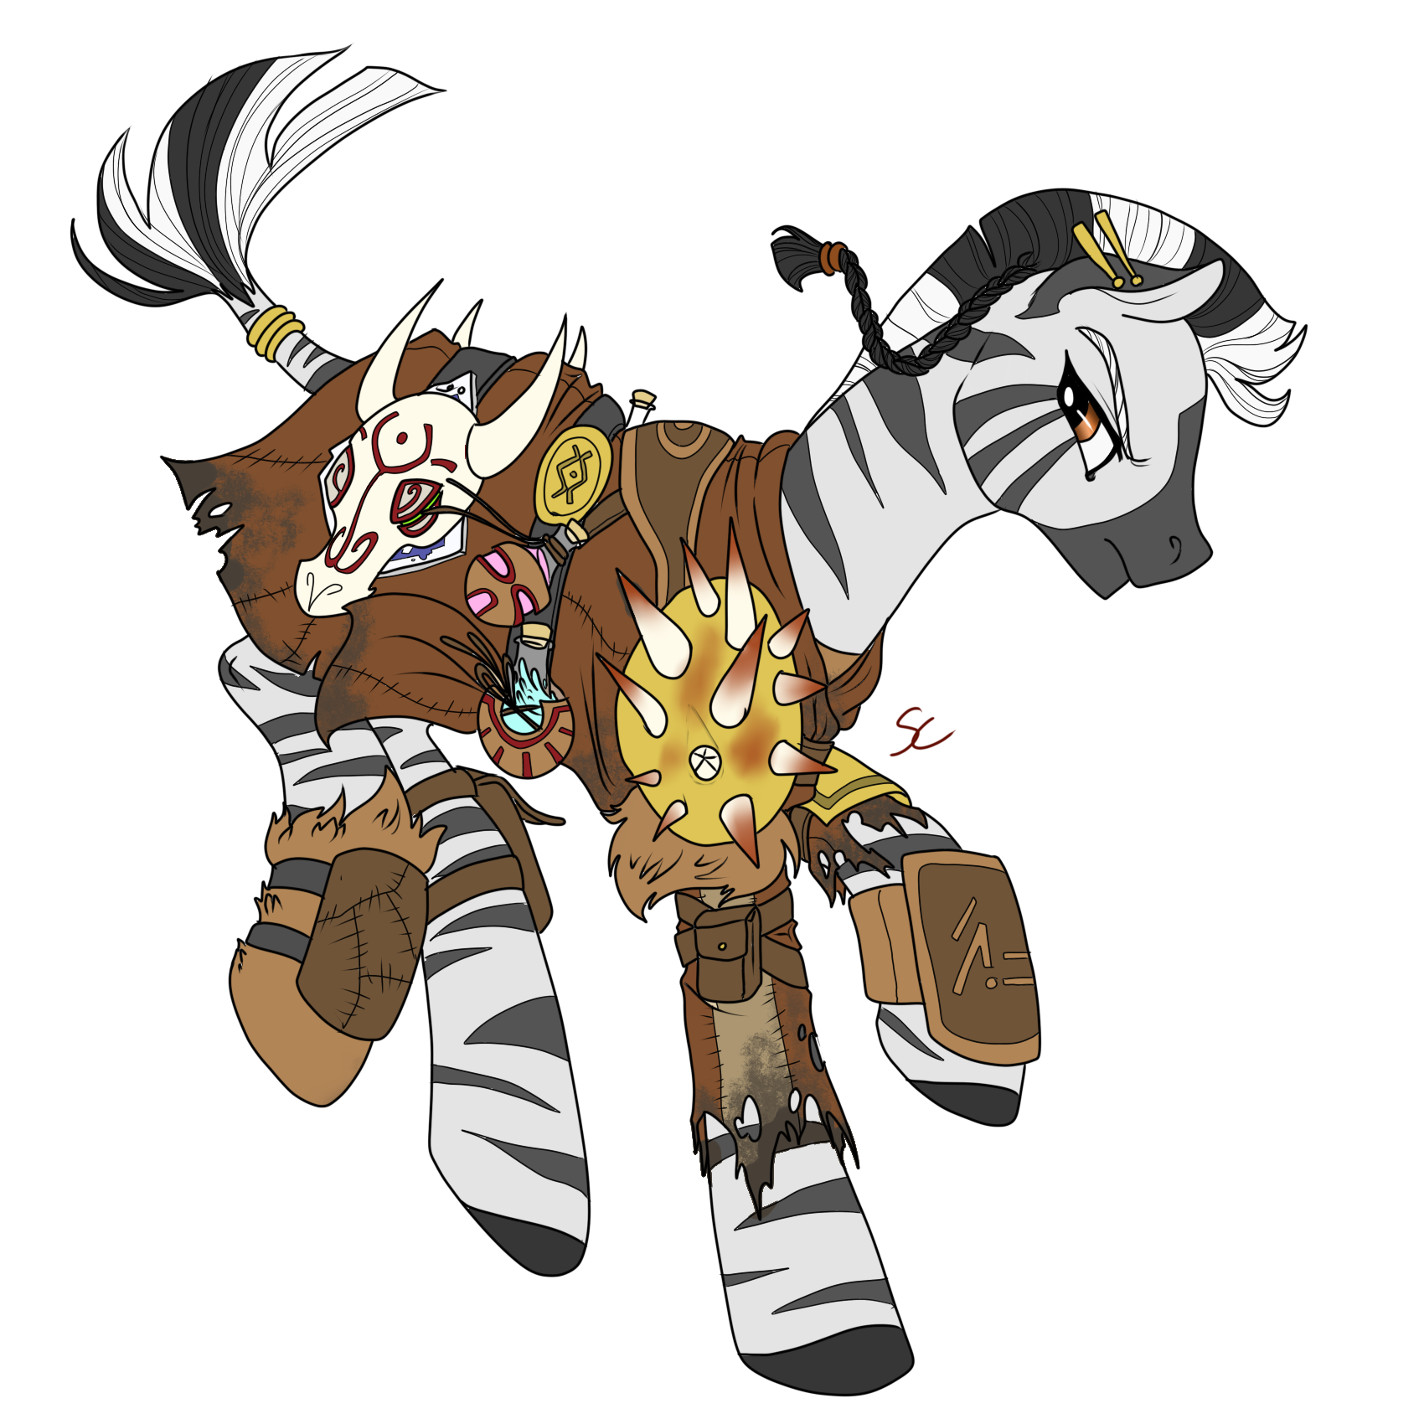
\includegraphics[width=0.8\linewidth]{ART/Races/ZEB_M}
	\end{figure}
	
	Zebras are distinguishable by their unique black-and-white striped coats and the glyph-like Cutie Mark that adorns their haunch. Their manes are also black and white in color. Close to their pony cousins, zebras have their own customs and methods of magic. Many zebras still cling to their beliefs, which seem preposterous and bizarre to many Equestrians, such as their fear of the stars.
	
	Zebras are capable of their own kind of magic; alchemy, the art of creating potions to alter one's self. In addition to this, some have acquired skills in dealing with the often-invisible spirits that inhabit the post-apocalyptic Equestria.
	
	It is entirely possible for a zebra to be both an alchemist and a shaman, though they must go through rigorous amount of training and personal sacrifices to do so.
	
	Zebras have the following racial abilities:
	\begin{description}
		\item[Glyph:] Zebras have a \textbf{Special Talent}, giving them +5 to a skill when using their special talent.
		\item[Tribal Concoctions:] Zebras can use alchemy, cooking brews and potions.
		\item[Witchy Wards:] Zebras are naturally resilient against arcane magic, giving them a +10 in opposed rolls made to resist a unicorn's spells. In addition to this, their long history with alchemy has given them a natural-built tolerance to poisons; their starting Poison Resistance is 20 instead of 10.
	\end{description}	
	
	\clearpage
	
	\section*{SPECIAL}
	\addcontentsline{toc}{section}{SPECIAL}
	The acronym ``SPECIAL'' is made from the primary statistics of the system - \textbf{Strength}, \textbf{Perception}, \textbf{Endurance}, \textbf{Charisma}, \textbf{Intelligence}, \textbf{Agility} and \textbf{Luck}. These attributes are the core of all characters that roam the Wastes; the natural strengths and weaknesses of the characters. What makes your character SPECIAL?
	
	SPECIAL values are expressed by a number between 1 to 10, with 5 being the average; the higher, the better. In some cases one's SPECIAL can raise above 10 thanks to various temporary effects, up to a maximum of 15.
	
	Permanent increases and decreases to SPECIALs are gained by Perks, Cybernetic Implants and Alchemy. Permanent changes to SPECIALs are not always retroactive, increasing or decreasing SPECIALs do not affect Skill Points and Spells from previous character levels.
	
	Temporary increase and decrease to SPECIALs exist, such as certain clothes or chems. Temporary buffs and debuffs always affect SPECIAL checks and opposed rolls using SPECIALs as well as \textbf{Potency} of spells. They do not affect \textbf{Skills}, but they can affect other stats, such as temporary increase in STR will increase one's \textbf{Carry Weight} and \textbf{Melee/Unarmed damage} momentarily. 
	
	\subsection*{Strength (STR)}
	A measure of your character's physical strength and muscle power. Characters with a high Strength probably spent a lot of time in the gym in high school. Characters with low Strength probably got beat up by the characters with high Strength. Rolls against Strength are used when characters try to break doors down, bend the bars on their prison cell, and do other feats that require sheer muscle power.
	
	\medskip 
	Affected by temporary changes:
	\begin{compactitem}
		\item 	Carry Weight
		\item 	Melee \& Unarmed damage
		\item 	Penalties from Min STR requirement
		\item 	Breaking free of Grapple
		\item 	Weight lifting
	\end{compactitem}

	\medskip
	Affected by permanent changes only:
	\begin{compactitem}
		\item Melee \& Intimidation skill values
	\end{compactitem}
	
	\subsection*{Perception (PER)}
	A measure of your character's awareness and ``street-smarts'', sometimes called instinct or a ``gut feeling''. Perceptive characters notice details instantly, like smells, sounds, and sights that don't fit a ``normal'' picture. Highly perceptive characters are private investigators or snipers. Characters with low Perception walk about in their own little world. Rolls against Perception are used when there is a little detail the character has a chance of noticing, such as the glisten off the scope of the sniper taking an aim at their head. 
	
	\medskip
	Affected by temporary buffs:
	\begin{compactitem}
		\item 	All five senses
		\item 	Detecting details
		\item 	General awareness of surroundings
	\end{compactitem}

	\medskip
	Affected by permanent changes only:
	\begin{compactitem}
		\item Explosives, Lockpick \& Magical Weapons skills
	\end{compactitem}
	
	\subsection*{Endurance (END)}
	A measure of your character's constitution and overall health. Characters with a high Endurance have great immune systems, good cardiovascular fitness, and can outrun and outswim others. Characters with high Endurance can swim across the Bay of Manehattan. Characters with low Endurance can drown in the kiddie pool. Rolls against Endurance determine things like whether your character can hang on to that rope over a canyon, or can resist the deadly cloud of bacteria some renegade scientist just sprayed in their face.
	
	\medskip
	Affected by temporary buffs: 
	\begin{compactitem}
		\item 	Healing Rate
		\item 	Resistances
		\item 	Aerial Maneuvers of flying characters (alongside AGI \& CHA)
		\item 	Holding one's breath
		\item 	General stamina
	\end{compactitem}

	\medskip
	Affected by permanent changes only:
	\begin{compactitem}
		\item 	Hit Points
		\item 	Survival \& Unarmed skills
	\end{compactitem}

	\subsection*{Charisma (CHA)}
	A measure of your character's manners, appearance and general likability. Charisma may also limit your ability to gain followers and also determines how well you resist magical attacks directed at your soul. Rolls against Charisma are made when a character is attempting to communicate without words, for example to frighten away animals, to see through bluff and to directly influence NPC's with appearance and mannerism.
	
	\medskip
	Affected by temporary buffs:
	\begin{compactitem}
		\item 	Aerial Maneuvers of flying characters (alongside AGI \& END)
		\item 	Spirit Affinity
		\item 	Social situations in general
		\item 	NPC Disposition
		\item 	Determines the player's maximum Insanity
		\item 	Convincing others with manners or body language (acting, intimidation, etc.)
	\end{compactitem}

	\medskip	
	Affected by permanent changes only:
	\begin{compactitem}
		\item Barter \& Diplomacy skills
	\end{compactitem}

	\subsection*{Intelligence (INT)}
	A measure of your character's higher reasoning power. Characters with high intelligence have better memories and are better at solving problems than characters with low intelligence. Rolls against Intelligence are made when characters are attempting to guess a password or determine the pattern sequence of electric charges running through the pattern on the floor.
	
	\medskip
	Affected by temporary buffs:
	\begin{compactitem}
		\item 	Determines the player's Maximum Insanity.
		\item 	Affects reading speed and use of Pre-War Books and Magazines
		\item 	Memory
		\item 	Intuition
	\end{compactitem}	

	\medskip
	Affected by permanent changes only:
	\begin{compactitem}
		\item 	Skill points on levelling up
		\item 	Mechanics, Medicine, Science and Thaumaturgy skills
	\end{compactitem}
	
	\subsection*{Agility (AGI)}
	A measure of your character's speed and quick actions. Rolls against Agility are made when your character dodges a falling tree or attempts to jerk their hoof out of the sewer before a mutated rat bites it off. 
	
	\medskip
	Affected by temporary buffs:
	\begin{compactitem}
		\item 	Action Points
		\item 	Initiative
		\item 	Aerial Maneuvers of flying characters (alongside END \& CHA)
		\item 	Breaking free of Grapple
		\item 	General dexterity and balance
	\end{compactitem}

	\medskip
	Affected by permanent changes only:
	\begin{compactitem}
		\item 	Firearms, Sleight \& Sneak skills
	\end{compactitem}
	
	\subsection*{Luck (LCK)}
	Perhaps the most ambiguous statistic, Luck is everything and nothing. Characters with a high amount of Luck just tend to have things go their way, and characters with a low amount of Luck always seem to be standing under the delivery cart when the piano is dropped. Rolls against Luck are made at the GM's discretion; Luck rolls can determine if, when your character is out of ammo and lying half-unconscious on the ground, he happens to find that loaded shotgun lying concealed and forgotten in the dust.
	
	\medskip 
	Affected by temporary buffs:
	\begin{compactitem}
		\item 	Critical success and failure thresholds
		\item 	Breaking free of Grapple
		\item 	Looting
	\end{compactitem}

	\medskip
	Affected by permanent changes only:
	\begin{compactitem}
		\item 	All skills slightly
	\end{compactitem}
	
	
	\section*{Secondary Statistics}
	\addcontentsline{toc}{section}{Secondary Statistics}
	These statistics are values that are either derived from your SPECIAL values or otherwise determine your character, the nitty-gritty of your character sheet.
	
	\subsection*{Level}
	Your character has a \textbf{Level} (lvl) measuring their experience and time in the Wasteland. Levels are gained through \textbf{Experience Points} (XP) rewarded throughout the character's journey from various actions; usually assigned during or after a game session by the Game Master.
	
	\subsection*{Hit Points}
	\textbf{Hit points }(HP) are one of the most important statistics in the game - they determine if your character is alive and walking or dead and buried. If a character's HP at any moment reaches 0, the character has perished.
	
	HP can recover with time, drugs, correct skills or a visit to your local doctor. Your maximum HP are determined by the following formula:
	\begin{center}
		$10+END$		
	\end{center}	
	HP is indicated by a column of tokens, called \textbf{Health Tracker}. Once character takes damage, their health begins to dwindle downwards.
	
	All characters have 10 HP as a base. The character adds their END to this for their Total HP. For example, a character with 5 END has a maximum of 15 HP.
	
	All characters have Pain Thresholds at 5 HP, 3 HP and 1 HP. When a character reaches these Pain Thresholds, further penalties are applied through statuses, to indicate that the character's bodily limit is being reached. These statuses are rolled by the GM from a table with various effects, meaning that not all characters begin to break down the same way.
	
	Pain Thresholds, HP Token loss and healing HP is further explained in Chapter 7: Combat - Dealing Damage.
	
	\subsection*{Healing Rate}
	Your body heals at a natural rate - albeit slowly. Healing Rate stat represents your character's natural healing process during at least 8 hours of rest.
	
	The character's Healing Rate is determined by their Endurance; characters with low END heal less Hit points than characters with high END, as shown below:
	\bigskip
		
	\begin{tabular}[h]{ll}
		END 1-3  & Heals 1 HP / 8 hours \\
		END 4-7  & Heals 2 HP / 8 hours \\
		END 8-10 & Heals 3 HP / 8 hours
	\end{tabular} 

	\subsection*{Action Points}
	Your\textbf{ Action Points} (AP) determine how quickly you act in combat - and how many actions you can perform in one combat turn. Action Points are determined by the following formula:
	\begin{center}
		$10+(AGI/2)$
	\end{center}
	Various perks and traits modify how many APs a character has and/or spends with specific actions. Be sure to keep note on the modifiers if you choose one.
	
	If you have AP remaining after having used all actions you wanted to use, the remaining AP doesn't carry over to the next turn. In other words, AP refreshes each turn.
	
	\begin{table}[b]
		\centering
		\rowcolors{1}{gray!30}{gray!10}
		\begin{tabu} to 0.8\columnwidth {| X[l] |}
		\hline
		\emph{\textbf{Design Note: AP explained}}\\
		\hline 
		\emph{Action points limit the number of actions characters can do within a turn and normally every action costs AP to prevent characters from acting indefinitely. As different actions are faster and simpler to do, AP prevents need of limiting characters to set amount of actions per turn.}\\ 
		\hline 
		\end{tabu}	
	\end{table} 
	
	\subsection*{Strain}
	\textbf{Strain} tells how long one can keep dishing out those special tricks, maneuvers, or spells a character possesses until burnout strikes. Essentially, this is your fatigue. All characters have a default Strain pool of 20, which increases by 5 every 5 levels. Characters regain all their Strain after 8 hours of rest.
	
	Unicorn and Earth pony magic, pegasi and griffons' Aerial Maneuvers, and zebra Alchemy all use up Strain due to them using the innate magic in them.
	
	Shamanism uses Strain far less than the above-mentioned magics, as it is only spent when crafting Runes. The act of calling and using Spiritual magic is Strain-free due to the Spirit's power being on loan to the Shaman rather than harnessed from the zebra's innate magic themselves.
	
	\subsection*{Skill Points}
	\textbf{Skill Points} are accumulated with each level up your character receives while wandering. The gaining of Skill Points follows the formula:
	\begin{center}
		$10+(INT/2)$
	\end{center}	
	A complete list of skills, their initial calculation and associated descriptions is provided under Chapter 2: Characters - Skills. 
	
	\subsection*{Karma}
	Unlike most Secondary Statistics, \textbf{Karma} is not derived from SPECIAL stats. It determines your character's moral alignment - it can and will change during play as determined by the GM from your character's actions, and the value will affect various characters' disposition on your character. One's karma value can range from -100 to 100 - between an immoral wasteland monster and a paragon of virtue, respectively. Karma value of 0 is the neutral middle-ground.
		\begin{table*}[t] 
		\centering
		\caption{Size Category Modifiers}
		\label{Table:2.1}
		\rowcolors{1}{gray!30}{gray!10}
		\begin{tabular}{|c|c|c|c|c|c|}
		\hline
		\textbf{			
			\textbf{		 
				Size }}&\textbf{ HP }&\textbf{ Hit Chance }&\textbf{ Carry Weight }&\textbf{ Reach }&\textbf{ \begin{tabular}{@{}c@{}}
					Combat Trick \\
					 Modifiers
				\end{tabular} }\\ \hline
			
			4 & +4 & +40 & +60 kg & 10 m / 5 hex & +40 \\ 
			
			3 & +2 & +20 & +40 kg & 4 m / 2 hex & +20 \\ 
			
			2 & +1 & +10 & +10 kg & 2 m / 1 hex & +10 \\ 
			
			1 & - & +5 & +5 kg & - & +5 \\ 
			
			0 & - & - & - & - & - \\ 
			
			-1 & - & -5 & -5 kg & - & -5 \\ 
			
			-2 & -1 & -10 & -10 kg & - & -10 \\ 
			
			-3 & -2 & -20 & -40 kg & - & -20 \\ 
			
			-4 & -4 & -40 & -60 kg & - & -40 \\ 
		\hline
		\end{tabular}	
		\end{table*}
	Besides NPC disposition, some spirits a zebra shaman can summon react differently to the summoner's karma.
	
	\subsection*{Insanity}
	The Wasteland is not a nice place. It will beat you down mercilessly and it will take a toll on your sanity. Certain spells, traumatic experiences, and damage to your mental capabilities can steer you towards insanity. \textbf{Insanity meter} is meant to gauge how well your character is taking in the brutality of Wasteland.
	
	When a character is about to get an Insanity point, they roll a 1d100. If the result is 20 or under, their sanity has worsened. There are certain perks that affect this roll, as well as methods to lower one's Insanity - such as certain Chems, spells, and alchemy recipes.
	
	Insanity meter is equal to your base Charisma or Intelligence, whichever is the higher stat. Should a character's Insanity meter reach maximum, the character will go insane and be removed from the player's control. It is at the GM's discretion if a character that has left play in this manner can be brought back.
	
	\subsection*{Size}
	Size category determines how large the character is. It ranges from -4 to +4, with most equines representing the middle size category of 0. Size category can be changed with Traits, Spells and Zebra Alchemy.
	
	Size category affects various statistics, as displayed on Table 2.1.
	Hit Points modifier represents the resiliency, that size brings to a character, while hit chance modifier represents the difficulty to hit the said character of either large or small size. Characters do not apply their own Size category's Hit Chance to the rolls when targeting others - only the opponent's Size will provide additional bonus or penalty.
 
	That is, a character with Size -2 does not gain a malus (or bonus) to their roll from Size when targeting a character with Size 0, while the opposite is true.
	
	Carry weight represents the total muscle mass that body has different body sizes affects the base values.
	
	Reach represents the length of one's body parts and affect the distance a character can hit with a swing from a club.
	
	Combat trick modifier affects how easy combat tricks can be performed by the character.
	
	\subsection*{Carry Weight}
	How much stuff your character can haul in his saddlebags without having to start picking what to drop. Every item weighs something. Carry weight is determined by the following formula:
	\begin{center}
		$10kg+(STR \times 5kg)$
	\end{center}
	The Carry Weight can be further modified by traits. Apply changes from them after calculating the base Carry Weight.
		
	If a character is carrying more than their Carry Weight allows, they are considered Encumbered. If they are carrying over double their Carry Weight, the penalties are doubled. Over triple their Carry Weight, the character is unable to move. When she removes the excess weight, the conditions immediately end.
	 
	\subsection*{Resistances}
	\subsubsection*{Fire, Cold \& Electricity}
	When out in the Wasteland, your character will face various environmental hazards. These hazards can be resisted in two ways: Elemental hazards, such as heat and cold, need a SPECIAL roll to resist harmful status effects from such attacks. Physical damage from these hazards are resolved like normal damage, with certain clothing and perks give extra DT to resist these types of damage.
	
	\subsubsection*{Poison \& Radiation}
	Poison and Radiation are somewhat rarer and have much more harmful effects. Radiation causes penalties to a character's ability to function the more the Rads they have, while poisons are more varied in their effects but do not accumulate.
	
	Defending from Poison or Radiation requires \textbf{Radiation Resistance} and \textbf{Poison Resistance} respectively. All characters start with a static value on both and they can further be modified with perks, Chems and apparel. Resistance lowers the likelihood of Rads or poison coming through by lowering the success chance; for example, a character with 5\% Rad Resistance can lower the incoming percentage by 5, thus 50\% becomes 45\% instead. The minimum chance to gain Rads is 5\%. These Resistance values do not alter how many times the chance is rolled at a given time.
	
	If a poison or radiation is delivered with a weapon, it requires the target to lose HP for the poison or Rads to get through. If the character's DT overcomes the weapon's damage, the poison or Rads haven't been inflicted. More information on losing HP tokens and DT can be found under Chapter 7: Combat - Dealing Damage.
	
	To check how Poison and Radiation damage is applied, check under Chapter 5: Game Rules - Environmental \& Other Hazards.
	
	The base values of the resistances are detailed on Table 2.2.
		
	\begin{table}[t]
		\centering
		\caption{Resistances and Their Base Values}
		\label{Table:2.2}
		\rowcolors{1}{gray!30}{gray!10}
		\begin{tabular}{|l|c|}
			\hline
			Resistance   &      Value      \\ \hline
			Poison       &      10\%       \\
			Radiaton     &       5\%       \\
			Cold         & END / AGI check \\
			Heat         &    END check    \\
			Electricicty & END / STR check \\ \hline
		\end{tabular}
	\end{table} 
	\begin{verse}
		\textbf{Example 1:} \emph{Doc Red has Radiation Resistance of 10 and is being attacked by a Glowing One's Irradiated Burst. The attack says that the burst is rolled 5 times, at 50\% probability. GM asks for Doc Red's Radiation resistance, meaning that the probability of the attack coming through is 50\% - 10\% = 40\% instead. GM rolls d100 5 times, of which two go under 40, meaning they have successfully been inflicted on Doc Red. Thus Doc Red takes 2 Rad tokens and adds them to the lowest available space on his Rad Tracker.}	
	\end{verse}	

	\begin{verse}
		\textbf{Example 2:} \emph{Emerald Glint fires up a Gamma Gun at their enemy, dealing radiation damage as: 2 x 40\% with 1 Rad Token inflicted. The enemy has a Radiation Resistance of 10\%, so the Gamma gun's damage changes into 2 x 30\%. Emerald Glint's player rolls 1d100 twice, and gets results 60 and 25. Of these, only one is under 30, so only one of the radiation attacks inflict damage on the target, giving the enemy 1 Rad token increase to their Rads meter.}
	\end{verse}

	\subsection*{Potency \& Spirit Affinity}
	\textbf{Potency} tells how powerful spells the spell-caster in question can throw at enemies or objects. Potency is only taken into account by unicorns. The following formula determines one's Potency:
	\begin{center}
		$lvl+(SPECIAL)$
	\end{center}
	The SPECIAL used in calculating Potency is determined by the Magic School of the spell.
	
	Some zebras are capable of Spirit Magic, also known as shamanism. They possess a unique statistic called \textbf{Spirit Affinity}, which determines the power of summoned spirits. The following formula is used to calculate a Shaman's Spirit Affinity:
	\begin{center}
		$lvl+CHA$
	\end{center}
	
	\subsection*{Aerial Maneuvers}
	\textbf{Aerial Maneuvers} are the skills that pegasi and griffons use in aerial combat. Aerial Maneuvers use AGI, END, or CHA depending on the maneuver. Pegasi start with 3 Aerial Maneuvers while griffons start with 2 Aerial Maneuvers.
	
	Pegasi learn a new Aerial Maneuver \textbf{every 5th level} (6, 11, 16) after first level and griffons learn a new Aerial Maneuver \textbf{every 6th level} (7, 13, 19) after first level.
	
	In addition to this natural learning, the Aerial Maneuvers can be learned during gameplay through a magazine, flight instructor and by self-taught training.
	
	In the Equestrian Wasteland, characters can sometimes find a copy of a flight magazine called \emph{``Aerodynamics Monthly''}. This magazine was published during the war to showcase the techniques used by Wonderbolts. Reading this magazine will teach 1 new Aerial Maneuver per magazine.
	
	To learn a new Maneuver by self-teaching, a character must succeed on a AGI/END/CHA -2 roll, depending on the Maneuver the character wants to learn. To learn a maneuver, the character must roll 4 \textbf{successful checks}, however, only one check may be made per day. The character may re-roll this check once per day. 
	
	Having a teacher to coach the character reduces the required successful checks from 4 to 2.
	
	Flight speed can be improved in place of taking a maneuver, with each improvement giving 2 meters (1 Hex) extra movement to flight speed.
	Aerial Maneuvers and their descriptions can be found in \textit{\textbf{Magic Codex}}.
	
	
	\section*{Skills}
	\addcontentsline{toc}{section}{Skills}	
	Your character's \textbf{Skills} reflect their various abilities and knowledge. The skill value indicates how good your character is at that skill. Skill values can be increased by allocating \textbf{Skill Points} at character creation and \textbf{Level Ups}. Skill values are normally expressed by a number between 1 to 85; the higher the Skill value, the better your chance of success.
	
	Once a skill has reached a total of 85 from a combination of skill points, Perks, Traits and Tags, no further skill points may be invested on it. Any bonuses above the skill cap, such as temporary ones from magazines, Chems and gear, can be used to compensate penalties character may have or gain during play.
	 
	The only method of increasing the skill cap of 85, is studying a skill related \textbf{Book}. The book-bonus raises the cap for that particular skill to 90. Knowledge is power, after all, and Books are based on effort and studies considerably longer than one's lifetime. In addition, if the character has a Special Talent, the +5 from it can also go over the hard cap.
	
	The starting value of each skill is equal to double the skill's associated SPECIAL plus half your LCK. The number of skill points the character receives at both character creation and level-ups is equal to $10 + (INT / 2)$.  This value is rounded down. In addition to this, the character has three Tagged skills, skills that she can have an extra +20 to make those rolls easier and to represent her talent with those skills in particular.
	
	\textbf{A character can assign a maximum of 5 skill points per skill per level.} 
	
	\subsection*{Barter}
	\textbf{Starting value:} $(2 \times CHA)+(LCK/2)$
	
	The Barter skill covers understanding of economics and trade, as well as dealings with spirits from the beyond. A good Barter skill isn't important if you're killing everyone, but it certainly is a valuable skill for the non-berserkers out there.
	
	Barter is primarily used in the buying and selling of items, such as trading with a merchant or scavenger, or exchanging mutual goods or favors.  This skill alters prices for purchasing and selling of items. Modifiers include factors such as condition of the item a character is trying to sell and NPC disposition towards said character.
	
	Barter is also the primary skill involved in shamanism.
	
	\subsection*{Diplomacy}
	\textbf{Starting value:} $(2 \times CHA)+(LCK/2)$
	
	The Diplomacy skill determines the character's verbal proficiency at persuading, talking her way out of combat, or convincing people to give up vital information. Diplomacy is also used for insight into the communication of others and catch hidden context.
	 
	Diplomacy rolls are usually used to augment roleplaying when dealing with NPCs. However, Diplomacy is not used to influence other players!
	
	\subsection*{Explosives}
	\textbf{Starting value:} $(2 \times PER)+(LCK/2)$

	The Explosives skill is used when the character tries to manipulate anything that can go boom in an instant - be it deliberately or not.
	Explosives determines the character's knowledge and accuracy with all mines, grenades, and weapons that launch explosive ordinance other than bullets - these weapons include missile launchers, grenade launchers and Balefire Egg Launcher (BEL).
	
	It also governs the character's prowess in the art of defusing and disarming explosives. With enough skill and right components, the character can also craft some form of explosives.
	
	\subsection*{Firearms}
	\textbf{Starting value}: $(2 \times AGI)+(LCK/2)$
	
	The Firearms skill is used whenever the character deals with weapons that fire gunpowder-based ammunition. Firearms are known to kick back after firing a shot.
	
	This skill determines the character's accuracy and prowess with all conventional firearms - like Hunting Rifle, 9mm Pistol and Minigun.
	
	\subsection*{Intimidation}
	\textbf{Starting value:} $(2 \times STR)+(LCK/2)$
	
	The Intimidation skill shows how frightening the character can act, utilizing not only her verbal prowess but her acting as well to make the opposition tremble. Sometimes when soft words fail, one must bring in the big stick to get to where she wants - and Intimidation fills that role.
	
	The skill determines how well the character can retrieve information from unwilling or afraid subjects, and make others fear her.
	\vfill
	\pagebreak
	\subsection*{Lockpick}
	\textbf{Starting value:} $(2 \times PER)+(LCK/2)$
	
	If the character needs to open locks without the proper key, this is the skill for her. A character may use it to get what she want, but others don't want her to have.
	
	The Lockpick skill governs the character's ability to pick conventional locks with the help of a screwdriver and a bobby pin or similar tools of trade.
	
	\subsection*{Magical Energy Weapons}
	\textbf{Starting value:} $(2 \times PER)+(LCK/2)$
	The Magical Energy Weapons skill (MEW) is used when the character uses weapons that fire magic-based projectiles, such as laser beams or goop of plasma.
	
	This skill determines the character's accuracy with all ranged magical weapons - for instance the Magic Energy Rifle, Plasma Pistol and Thunder Cannon.
	
	\subsection*{Mechanics}
	\textbf{Starting value:} $(2 \times INT)+(LCK/2)$
	
	As things are constantly breaking in the wastes, and there aren't customer service hot-lines anymore. A person with a high Mechanics skill is always good to have around.
	
	The Mechanics skill determines the character's ability to build, repair and modify items, as well as to disable machines and non-explosive traps. It is also used in the scavenging of useful parts from machinery and robotics.
	
	\subsection*{Medicine}
	\textbf{Starting value:} $(2 \times INT)+(LCK/2)$
	
	The ability to protect life can be just as important as the ability to take life. The Medicine skill represents a character's medical training as well as basic biological intuition and the ability to properly diagnose causes of illness and wounds that are not immediately apparent.
	
	Outside of healing potions, which are the quick but costly fix to the injured, a medical practitioner can heal others with a successful Medicine check. Details on how to heal others with Medicine is found under Chapter 7: Combat - Damage Calculations.
	
	\subsection*{Melee}
	\textbf{Starting value:} $(2 \times STR)+(LCK/2)$
	
	The Melee skill determines your character's prowess with weapons designed to keep enemies from a leg's length away from you - while still swatting at them with abandon.
	
	This skill is used whenever the character attacks with a close-quarter combat weapon such as a baseball bat, magic energy spear, and chainsaw. This skill is also used with non-explosive thrown weapons like javelins, shuriken or throwing knives.
	
	\subsection*{Science}
	\textbf{Starting value:} $(2 \times INT)+(LCK/2)$
	
	Sometimes there's an electronic lock in place of a mundane one or an automated defense system protecting a building. In these situations, it is time to bring out the computer nerd to clear one's path.
	
	The Science skill determines the character's grasp of mundane and arcane sciences. Science governs a character's ability to invent, hack terminals, as well as the character's ability to operate and understand of pre-war technology.
	
	\subsection*{Sleight}
	\textbf{Starting value:} $(2 \times AGI)+(LCK/2)$
	
	The Sleight skill shows how good the character is with her hooves or claws and how nimble her fine motor skills are. With high Sleight skill she could build a tiny house from matches without a problem, slide out of ropes keeping her down, or slip caps out of an unsuspecting passerby's pocket.
	 
	Sleight skill also determines how well you slip concealed weapons into establishments unnoticed.
	
	\subsection*{Sneak}
	\textbf{Starting value:} $(2 \times AGI)+(LCK/2)$
	
	The skill of being able to move quietly or out of sight. When a character is sneaking, other characters will be less likely to notice her at a distance. Masters of this skill can deal deadly blows from the shadows or daring thievery without the foes being any wiser of an intruder.
	
	The Sneak skill determines the character's proficiency at remaining undetected. This skill is also used to liberate a person out of their prized possessions while they're standing in the same room.
	
	\subsection*{Survival}
	\textbf{Starting value:} $(2 \times END)+(LCK / 2)$
	
	The Survival skill is the skill of outdoor living and survival in hostile environments. Basically what they teach in Filly Guide, modified for the post-War world. Survival has many uses: from finding food and water in the middle of a vast wasteland, to avoiding hostile creatures' domains, to knowledge about what plants and animals will be helpful or harmful.
	
	The Survival skill determines the character's overall wasteland savvy and her proficiency at cooking, scavenging, tracking, and crafting ``natural'' equipment and consumables.  Survival informs a character about weather, geography and orientation.
	
	Survival also determines how skilled a zebra character is at Alchemy and helps determine what brews and salves an alchemist can create with the right ingredients.
	
	\subsection*{Thaumaturgy}
	\textbf{Starting value:} $(2 \times [SPECIA])+(LCK/2)$
	
	Each pony has inherent magic in them, and the Thaumaturgy skill shows how well they have mastered that. For unicorns, it's their reliability of spells; for pegasi, their maneuvers; for Earth Ponies, their touch with the earth.
	
	Thaumaturgy determines how well the character can do her race's inherent magical capabilities and their general knowledge of the subject. As each pony's magic and how they handle it is unique, there's no specific SPECIAL value linked to Thaumaturgy. During character creation, one SPECIAL value, Luck excluded, is attached to Thaumaturgy to calculate the starting value.
	
	\subsection*{Unarmed}
	\textbf{Starting value:} $(2 \times END)+(LCK/2)$
	
	Firearms can jam, and melee weapons can be broken. At this point, it helps to utilize the natural weapons - hooves and claws.
	
	The Unarmed skill determines the character's accuracy in unarmed or martial combat, as well as weapons worn directly on one's legs - for example horseshoes and Power Glove. Further details on Unarmed Weapons can be found under Chapter 3: Equipment - Weapon Characteristics.
	
	\vfill
	\pagebreak
	
	\section*{Traits}
	\addcontentsline{toc}{section}{Traits}	
	Traits are the character's good and bad habits or quirks, making the life for the character a bit tougher or easier depending on the situation and the traits chosen. The Traits' purpose is to bring out a character's personality or background in a way that is not purely just for roleplay.
	
	A character may have up to two Traits.
	
	\subsection*{A Mazing Traveller}
	
	Travelling across the Wasteland is a wondrous thing although a bit disorienting at times. All character's movement actions cost 1 AP less, to a minimum of 1 AP, and ignores movement penalties of one Crippled limb. However, her mind suffers a disorienting penalty of -1 to her INT and PER.
	
	\subsection*{Aerial Ace}
	
	\emph{\textbf{Pegasus-only trait.}}
	
	The character is at home while in the air. On the other hand, while on the ground, she feels wobbly and often fumbles with physical tasks.
	
	She gains an additional Aerial Maneuver, maneuvers cost 1 less Strain (minimum 1 Strain), and she can move an additional 2 meters (1 hex) for 1 AP while flying in combat. However, she suffers a penalty of -10 to all STR, END and AGI based skills while on the ground or hovering slightly above it. These penalties do not apply while she's on clouds.
	
	\subsection*{Bad to the Bone}
	
	The moment the character was born, everyone around them knew that they were not to mess with the character. The character's \textbf{Explosives}, \textbf{Firearms}, \textbf{Intimidation},\textbf{ Magical Energy Weapons}, \textbf{Melee} and \textbf{Unarmed} skills are all increased by 5. The character's \textbf{Barter}, \textbf{Mechanics}, \textbf{Medicine}, \textbf{Science}, \textbf{Diplomacy} and \textbf{Survival} skills are all decreased by 5.
	
	\subsection*{Blueblood}
	
	The character is as beautiful as prince Blueblood or Fleur de Lis, but she is a lot less resilient than a "normal" pony. The character gains 1 CHA and +5 Diplomacy but suffers END -2 against Status Effects and poisons.
	
	\subsection*{Chem Reliant}
	
	For as long as the character remembers, she's been surrounded by a myriad of chems for all occasions. The character's chance of addiction when taking chems is doubled, but she will only suffer withdrawal effects after 48 hours of taking chems.
	
	\subsection*{Chem Resistant}
	
	The character's body has developed methods against the harmful drugs Wasteland has to offer, effectively purging the system of them. The character's chance of addiction is halved, but so is the duration of chems.
	
	\subsection*{Dashite}
	
	\emph{\textbf{Pegasus-only trait}.} 
	
	Character was once a member of the Grand Pegasus Enclave, but have since been given the boot and driven to exile. Thankfully, they were nice enough for them keep their gun...
	
	The character starts out with an Enclave Hailgun shotgun for free but is branded as a traitor amongst her peers and no longer has a cutie mark, rendering Special Talent bonuses moot.  \textbf{This trait is subject to GM approval. }
	
	\subsection*{Deep Sleeper}
	
	The character sleeps more soundly than most, making the most of her beauty sleep. The character regains double their Natural Healing Rate when resting for 8 hours. In addition, their Strain pool is increased by 5 permanently. 
	
	Unfortunately, the character automatically fails PER checks to wake up unless she takes damage, or someone spends a full turn waking her up. Likewise, it can be surmised that a character with this trait likely isn't going to be a morning person...
	
	\subsection*{Fast Shot}
	
	Why spend precious time aiming when you can pepper the field with fire? The character's attacks with firearms and magical energy weapons cost 1 less AP, though no less than 1 AP.  However, she cannot Aim or do Called Shots with firearms or magical energy weapons.
	
	\subsection*{Four Eyes}
	The character's effective PER for sight-related checks increases by 1 while wearing glasses or sunglasses. Whenever not wearing glasses, she suffers a penalty of -1 to her effective PER for sight-related checks in addition to bonus lost by not wearing glasses. The character has glasses in her inventory for free.
	
	\begin{verse}
		\textbf{Example:} Emerald Glint appears to have a poor eyesight, and wears glasses. With a base PER of 5, she has effective PER of 6 with glasses. However, if she drops her glasses her effective PER drops to 4.
	\end{verse}

	\subsection*{Gambling Caster}
	
	\emph{\textbf{Unicorn-only trait}}
	
	Some unicorns never truly grow out of their experimenting phase, leading to their magic manifesting in random, strange ways. Often with spectacular results. 
	
	Her \textbf{Potency} is calculated by using LCK. Instead of selecting individual spells, the character chooses \textbf{Magic Schools} she can cast from, up to 3. One of the schools has to be General Magic School. Spells cost 2 less AP and Strain to cast to a minimum of 1 each. On 10th level, the character may choose a new Magic School to his collection. 
	
	However, each time the character wants to cast a spell, she chooses one of the schools to cast from. The GM then randomly determines what spell the character has conjured. The GM will also tell the associated AP and Strain costs. 
	
	\textbf{This trait is subject to GM approval.} This trait is not recommended for new players.
	
	\subsection*{Ghoul}
	
	The character was mutated by the necromantic energies that were unleashed on Equestria in the apocalypse. This mutation has caused her to have an unnaturally long life, often having been alive during the war. 
	
	Most NPCs have a lower \textbf{Disposition} towards her, and they are ignored by ferals as long as they remain unprovocative. She heals through radiation, converting Rad tokens to HP tokens, but has a natural \textbf{Healing Rate} of 0. Accumulated Rads dwindle from a ghoul's body at the rate of 2 per day due to Ghoul's body using Rads to function.
	  
	After at least 8 hours of rest, the ghoul may choose to discard 2-5 Rad Tokens, and replenish an equal amount of HP Tokens and/or Crippled Conditions, if any are present.
	 
	If the character loses all of her Rads, she becomes vulnerable to physical deterioration; she must remove 1 HP token per day, each day she doesn't have enough Rads. This token cannot be replenished with Medicine checks. 
	
	When a ghoul reaches maximum amount of Rads, they will gain one point of Insanity per day. Upon gaining Insanity, the ghoul gains Enraged-status; if in combat, this lasts as long as the status usually lasts, and outside of combat for a moment seen appropriate. Should a Ghoul's Insanity be maxed, they turn feral, and are removed from the player's control. 
	
	Ghouls, due to their severely slowed metabolism do not need to eat or drink as often as regular ponies do; if Hunger and Thirst rules are in effect, they require one meal per 2 days and a drink per day to satisfy their needs.
	
	\subsection*{Good Natured}
	
	You have the manners and the face of a cherub! The character's \textbf{Barter}, \textbf{Mechanics}, \textbf{Medicine}, \textbf{Science}, \textbf{Diplomacy} and \textbf{Survival} skills are all increased by 5. The character's \textbf{Explosives}, \textbf{Firearms}, \textbf{Intimidation}, \textbf{Magical Energy Weapons}, \textbf{Melee} and \textbf{Unarmed} skills are all decreased by 5.
	
	\subsection*{Grounded Bird}
	
	\emph{\textbf{Pegasus/Griffon-only trait.}}
	
	The character is not considered a smooth flier. Instead her movements in the air are stiff and rough, and she has spent her life working against said deficiency.
	
	The character's Flying movements and Maneuvers cost 2 AP more. Her END is increased by 1.
	
	\subsection*{Hard Drinker}
	\emph{\textbf{Earth Pony -only trait.}}
	
	The character is the life of the party - when drunk, that is -, and has a permanent addiction to alcohol.
	
	Alcohol's positive effects and duration are doubled, and the character doesn't have to roll for END for ForeverPure. However, negative effects are unaltered, and she suffers from double the normal withdrawal effects whenever she is not under the influence.
	
	In addition, Hard Drinker has often a very distinct (bad) odor, which in tandem with her general appearance often causes other ponies to shun her; NPC dispositions are lowered by one level.
	
	\subsection*{Hard of Hearing}
	
	The character's hearing isn't quite on par compared to others, for good or ill. The character ignores 10 penalties from distractions that rely on sound, but suffers a -1 to spot sneaking enemies.
	
	\subsection*{Heavy Hoofed}
	
	The character has strength behind her blows - now if she also managed to hit quickly, it would be ideal. The character adds 2 to the STR multiplier when dealing Melee and Unarmed damage, but her Melee and Unarmed attacks cost 2 AP more.
	
	\begin{verse}
		\emph{\textbf{Example:} Shining Example is Heavy Hoofed and strikes a foe with her bare hoof. Normally STR multiplier for bare hoof is 2, but being Heavy Hoofed, Shining Example's multiplier would be $2+2=4 \times STR$.}
	\end{verse}
	
	\subsection*{Hoarder}
	
	The character has learned to pack everything in her pockets - because she wants it all, be it a nice new weapon or dried-up Wonderglue for the adhesive! The character has an increase of 20kg to her \textbf{Carry Weight}.
	
	However, the GM can ask for the character to roll for INT or CHA to resist her urges whenever she is carrying less than 30kg worth of \st{treasures} items. This is more likely the lighter the character's load is.
	
	\subsection*{Jinxed}
	
	You just have a bad streak of luck. Royally so, in fact. Thankfully, so does everyone around you. When you or your enemy rolls a critical fail, they experience the WORST. POSSIBLE. THING! Instead of their gun jamming, it explodes in a comical way, much like old-timey cartoon-slapstick and so on. 
	
	\subsection*{Kamikaze}
	
	You are fast to react and charge to battle, not giving a buck about the flying lead that whizzes past your ear. The character gains 2 Action Points but enemies gain a bonus of 10 to attacks made against the character.
	
	\subsection*{Large Frame}
	
	The character is a hulking figure and has strength behind her, though more often than not doorframes are her worst enemy.
	
	The character gains +2 STR. However, her Size category is increased by 1, making her an easier target.
	
	A character cannot have both \textbf{Small Frame} trait and \textbf{Large Frame} trait.
	
	\subsection*{Magic Knack}
	
	The character is proficient with a specific type of magic, being better than most in it. However, this leaves her skills lacking with other magic types. The character has +2 effective \textbf{Potency} in one \textbf{Magic School}. However, the other spells have -2 effective Potency.
	
	\subsection*{One Trick Pony}
	
	\emph{\textbf{Unicorn-only trait.}}
	 
	Unlike most Unicorns the character can only cast a single spell. Lucky for her, she casts that one spell very well!
	
	The character chooses only one spell at the begin of play. She cannot learn new spells on level up or otherwise. Instead, her Potency is as follows:
	\begin{center}
		$2 \times lvl+(SPECIAL)$
	\end{center}
	Also, One Trick Ponies have double the standard Strain pool size, at 40.
	A character may not have both \textbf{Spread Thin} trait and \textbf{One Trick Pony} trait.
	
	\subsection*{Paranoid}
	
	You think everything and everyone is out to get you. Because of this, you rarely put your guard down, expecting the worst to occur. However, this has made you quick on your feet; You have an additional +1 to PER and AGI, but your crazed ramblings of shadow mares that are out to get you impact your social standing. In exchange, your NPC disposition is lowered by 1.
	
	\subsection*{Random}
	
	\emph{\textbf{Earth Pony/Zebra-only trait.}}
	
	The character's innate magic manifests more overtly than is normal for her race. She is capable of performing cartoonish, impossible feats - such as using a squirt gun to successfully defeat a raider wearing power armor or handing a lit dynamite to a pony and walking away.
	
	The exact nature and limitations of the character's abilities are determined by the GM. These abilities are never reliable, and the GM may overrule any manifestation of random that they consider overused, abusive or excessively advantageous. \textbf{This trait is subject to GM approval.}
	
	A zebra with this trait cannot take \textbf{Tribal Shaman} trait.
	
	\subsection*{Rock Based Diet}
	
	\emph{\textbf{Earth Pony -only trait.}}
	
	The character is considered to have a lead-lined stomach and teeth of steel. She has learned to gain nutrition from where there is practically none, such as rocks, dirt and twigs.
	
	The character can consume nutrient-poor and barely edible materials, replenishing 1 HP. She may sustain this diet for up to END days without proper rations until falling unconscious.
	
	However, each day the character enjoys at least one of these ``lavish'' meals, all of her Resistances are reduced by 5.
	
	\subsection*{Scrooge}
	
	\emph{\textbf{Griffon-only trait.}} 
	
	The character has a dream - to collect such a wealth of Caps that she can dive around them like a porpoise, burrow through them like a gopher, and occasionally toss them up and let the Caps hit her on the head. Because no one is poor when they're doing something they like, are they?
	
	The character gains a bonus of 10 to Barter. However, her Diplomacy is lowered by 10. In addition, the character wants to get the best deal - every time. All prices are negotiable.
	
	\subsection*{Sex Appeal}
	
	The character has the ``right'' stuff. Individuals who are sexually oriented towards the character's gender are attracted to them, but potential sexual rivals tend to become quite jealous. 
	
	Those who would be attracted to a character with this trait have their disposition towards them - and only them - raised by one level, but potential sexual rivals will have their disposition lowered by one level.
	
	\subsection*{Small Frame}
	The character's life is to be taunted by high shelves. And sometimes, even the middle shelves. But at least she's fast, right?
	
	The character gains +1 AGI and her Size category is reduced by 1, making her a harder target. However, her limbs are 10\% easier to cripple.
	
	A character cannot have both \textbf{Large Frame} trait and \textbf{Small Frame} trait.
	
	\subsection*{Small Town Zebra}
	\emph{\textbf{Zebra-only trait}}
	
	The character hails from a small town or tribe, having thus learned the intricacies of communities where everyone knows each other.
	
	A character with this trait has a bonus of 10 to \textbf{Barter} and \textbf{Diplomacy} when dealing with NPC's of a small community. When dealing with a large organization or group - such as NCR or Steel Rangers - the character has a penalty of 10 to the same skills.
	
	The GM determines what is considered a small or large community.
	
	\subsection*{Spiritually Awakened}
	
	The character is gifted with the ability to see and communicate with spirits and ghosts who are normally imperceptible. The character's attunement to the spirit world makes them naturally well-disposed with ghosts and spirits, granting a +10 to Barter and +1 to CHA for purposes of talking to ghosts and spirits.  This bonus to CHA factors into a shaman's \textbf{Spirit Affinity} rating.
	
	However, the spirits also acknowledge the character's existence, trying to contact and bother her at both convenient and inconvenient times - be it during lunch, when trying to sleep, or ``going behind the bushes''.
	
	\subsection*{Spread Thin}
	
	\emph{\textbf{Unicorn-only trait.}}
	 
	The character's breadth of ability is second to none. If her spells weren't so weak, she could change the world!
	
	The character can choose up to 6 spells at character creation in addition to \emph{Telekinesis} and \emph{Light}.
	
	However, her Potency is less than normal, according to the formula below:
	\begin{center}
		$[lvl+(SPECIAL)]/2$
	\end{center}
	A character may not have both \textbf{Spread Thin} trait and \textbf{One Trick Pony} trait.
	
	\subsection*{Stable Dweller}
	
	The character starts the game with a PipBuck. Her starting Survival score is only $LCK/2$ and her starting Poison and Radiation Resistances are 0. 
	
	\textbf{This trait is subject to GM approval.}
	
	You can check PipBuck rules under Chapter 6: Additional Rules - PipBuck.
	
	\subsection*{Steel Ranger Outcast}
	\emph{\textbf{Earth Pony or Unicorn-only trait}}
	
	The character has been driven out or voluntarily left from Steel Rangers or Applejack's Rangers. This means that she starts play with Power Armor Training  -perk but is considered to be -1 NPC disposition for these factions, as she is considered to be a heretic and a traitor.
	
	\textbf{This trait is subject to GM approval. }
	
	\subsection*{Talon Mercenary}
	\emph{\textbf{Griffon-only trait.}}
	
	The character is either an active or a former Talon Company mercenary. The character gains the \emph{Bounty Hunter} -perk for free, but \textbf{NPC Disposition} is considered one level lower towards this character when discussing contracts of any kind.
	
	\textbf{This trait is subject to GM approval.}  At the GM's discretion, the character may start out with access to a suit of Talon Flight Armor.
	
	\subsection*{Tribal Shaman}
	
	\emph{\textbf{Zebra-only trait.}}
	 
	The character is a practitioner of zebra shamanism in the way of her ancestors, and benefits from ancient spirit pacts. The character starts with a \textbf{Spirit Affinity} score equal to $lvl+(CHA)$. She has an effective +2 Spirit Affinity with a particular type of Spirit of her choice, and an effective -2 Spirit Affinity with another type of Spirit of the GM's choice. Which spirits are the favorite and unfavorite do not have to be made known before they're encountered, if so desired.
	
	The character has access to Spirit Magic part of Zebra Magic, found in the \emph{\textbf{Magic Codex}}.
	
	\subsection*{Trigger Discipline}
	
	Why waste ammo, when you can deal more carnage with less? The character can reroll Called Shots when using firearms and magical energy weapons, but using them cost 1 more AP.
	
	\chapter{Equipment}
	
	\noindent
	Sometimes the difference between life and death comes down to the gear the wastelander is using. And as the Wastes care very little for your survival, and the beasts that roam it even less, one would find it wise to gear up when the possibility comes their way. Say, that caravan looks like it was recently stocked...
	
	In the following section are listed the gear that is provided within the Wasteland, but nothing stops you from creating your own.
	
	Full list of weapons, apparel and items can be found in \emph{\textbf{Wasteland Wares}}.
	
	Below are notes that rise up often in the following section.
	\begin{description}
		\item[Ammo:] 	Most ranged weapons require a specific ammunition type to deal damage. Refer to this when shopping for bullets for your gun or checking if ammo from one gun fits another.
		\item[AP Cost:] How much AP it takes to fire or swing with the weapon once.
		\item[Blast Radius:] With explosives and other similar weapons, Blast Radius determines the area of effect where the damage or other effect is applied, utilizing Burst Templates.
		\item[Capacity:] This determines the maximum amount of ammunition the weapon can hold.
		\item [Condition:]	\emph{[Optional Rule]} All pieces of equipment have a condition, describing their overall integrity and ability to function. Equipment lose condition through wear and direct damage dealt to them, and can be Repaired.
		\item[Damage:] Damage is listed as a combination of a base damage and a number of d10 dice to be thrown, shown in parenthesis. Ranged weapons have static damage, i.e. 20+(5), while Melee and Unarmed weapons account the character's STR value as a multiplier, determined by the weapon's statistics i.e. STR*2+15+(4)
		\item[Damage Over Time (DOT):] Certain weapons and spells cause DOT, such as burning, bleeding, poison and arcane damage. DOT is applied every round after initial damage, on the turn of the character that suffers from such effect. DOT ends after certain number of turns, indicated within action, weapon or spell description, or ended with a counter action by the victim or aiding character.
		
		The character takes DOT if the initial damage was above their corresponding DT or Resistances. DOT ignores DT and Resistances from armors, and clothing, as attack is considered to have breached armor or clothing. For instance, a blade that deals damage has punctured the hide and causes bleeding despite armor.
		\item[Damage Threshold (DT):] The value which tells how well the piece of gear protects you from attacks, reducing incoming Damage equal to the DT.
		\item[DT Reduction:] Weapons that have this value ignore the specified amount of opponent's DT.
		\item[Effect:] A passive, either constant or situational, effect granted by the equipment. These include but are not limited to: SPECIAL and Skill bonuses and penalties, AP cost modifiers, additional damage types and health restoration.
		\item[Firing Mode:] Ranged weapons vary how they operate. Each firing mode has its own characteristics. More information on different firing modes can be found in this chapter under Weapon Characteristics - Firing Modes.
		\item[Quick Slot:] A pocket, strap or holder in a piece of clothing and armor to hold quick accessible items, such as medicines, grenades and tools. More information on Quick slots can be found in this chapter under \emph{Quick Slots}.
		\item[Range:] This lists the weapon's Short, Medium, and Long range. All ranges are in meters. Weapon ranges are ``effective'' ranges for the purposes of the game. More on range can be found in Chapter 7: Combat - Combat statistics.
		\item[Reach:] Melee and Unarmed weapons can have reach, allowing them to deal damage against enemies from further away than adjacent hexes. This is noted with ``Melee / X m'' as Short range, where the latter value is the reach.
		\item[Reload Type:] This determines the magazine used by weapons that consume ammunition. There are four types of reloads with their own characteristics. More information on different reloads is listed in this chapter under Weapon Characteristics - Reload Types.
		\item[STR Requirement:] When the character has less STR than the minimum requirement for the weapon as specified in the weapon's statistics, she gains a cumulative penalty of -5 to accuracy and an additional cost of 1 AP to attacks for each lacking point of STR. The lacking STR on ranged weapons can be compensated by Bracing the weapon.
		\item[Type:] Lists in which weapon category said weapon belongs to. This is used to determine effects from perks and traits, like \emph{Jury Rigging}.
		\item[Value:] The weapon's usual rate in caps.
		\item[Weapon Slot:] A holster or strap where one can store her weapon, easily accessible for quick switch in a combat. More information on Weapon Slots is found in this chapter under Weapon Slots.
		\item[Weight:] How much the weapon weighs in one's inventory.
	\end{description}	
	
			
	\section*{Caps \& Currency}
	\addcontentsline{toc}{section}{Caps \& Currency}
	The character just cannot take all the stuff she wants from a store. Unless she wants her behind get peppered by a shotgun she must pay her purchases somehow, either bartering in her own ``junk'', or putting some currency as a balance. Because often bartering one item for another isn't a fair deal, a currency slowly developed to fill that gap.
	
	In the early days of war-afflicted Wastes, this currency was the most vital resource for survival - water. In time, pre-War bottlecaps, commonly known as caps, took this role. They are hard to counterfeit and there's a stable pool of them in circulation, only occasional new one being added with each pop of a Sparkle-Cola being opened. However, one should never rely solely on caps as only currency, for various people can still demand something of tangible use as their currency of trade.
	
	Sometimes one can come across little round pieces of bright metal coins, Bits. This was the currency used during the war, but it fell out in favor of bottlecaps, and is now mostly only good for melting down to something more useful.
	
	\textbf{The starting Caps for players is 500 caps.}
	
	
	\section*{Quick Slots}
	\addcontentsline{toc}{section}{Quick Slots}
	Some kinds of armor and clothing (especially belts) have easily accessible pockets, straps, or holders called \textbf{Quick Slots (QS)}. The number of Quick Slots is determined in the statistics of the armor or clothing. Quick Slots can hold only one item each, such as one knife, one grenade or one healing potion. The item must be small enough to fit in and weigh up to 1 kg. The GM determines if the item fits in the Quick Slot.
	
	Retrieving an item from a Quick Slot is much easier and quicker than from inventory thus costs only 3 AP.
	
	\begin{verse}
		\emph{\textbf{Example:} Maabara would like to have health potions readily available when things get chunky. She puts two healing potions into her two Quick Slots - as each Slot can only hold one item, she puts them in Slots 1 and 2. Thus instead of using 8 AP to fetch one from her inventory, she can take a healing potion from a Quick Slot with a cost of 3 AP.	}	
	\end{verse}
	
	
	\section*{Weapon Slots}
	\addcontentsline{toc}{section}{Weapon Slots}
	Each character has two Weapon Slots which can hold one weapon each. If a throwable weapon such as grenades or throwing knives are slotted in a Weapon Slot, every one of said weapon are equipped there. For example if the character has 15 frag grenades and puts said grenades in the weapon slot, he has access to all of them without having to access Inventory. Unlike \textbf{Quick Slots}, Weapon Slots do not have a limit on weight and they are not dependent on equipment.
	
	Retrieving a weapon from a Weapon Slot is much easier and quicker than from inventory and only costs 3 AP. For each use of throwable weapons a \textbf{Ready Weapon} action must be taken.
	
	\begin{verse}
		\emph{\textbf{Example:} Emerald Glint has equipped a Gretta M9 pistol in her first Weapon Slot and four frag grenades in her other Weapon Slot.  She takes out one of the frags and throws it. This means Emerald Glint first uses 3 AP from her total AP for Ready Weapon. Then, she uses another 3 AP due to frag grenade's Weapon AP cost. In total, Emerald Glint uses 6 AP to throw a frag grenade. After throwing the first grenade, she grabs another one. Again, Emerald Glint will use 3 AP to Ready Weapon and 3 AP to throw the grenade.}
	\end{verse}
	
	
	\section*{Weapon characteristics}
	\addcontentsline{toc}{section}{Weapon Characteristics}
	Apart from mere damage, weapons use varying ammunitions, clip sizes, firing modes, and range. The weapon types act as a defining factor, mainly for perks and other combat rules.
	
	Most ranged weapons and explosives have limited ammunition with various effects. As with weapons, ammunition has different rarities and pricing, making some more sought after, while others more commonly stumbled upon on many traders and old world heaps of supplies.
	
	\subsection*{Reload Types}
	\subsubsection*{C - Clip}	
	Clip is a removable container for ammunition. Capacity indicates the maximum amount of ammunition the clip can hold. Weapons that use clips usually come with an adequate number of suitable clips. On a reload action the current clip is removed, and a new clip is inserted. The AP cost for the entire reloading operation is determined by the weapon's statistics, under Reload AP.
	
	\subsubsection*{I - Internal magazine}
	Weapon with internal magazine has a storage for its ammunition built inside the weapon itself. Capacity indicates the maximum amount of ammunition the internal magazine can hold. On one reload action one piece of ammunition is inserted into the magazine. The AP cost for this is determined by the weapon's statistics, under Reload AP. If one wishes to fully reload a weapon, one has to take several reload actions.
	
	\subsubsection*{CY - Cylinder}
	Weapons with cylinder magazine hold their ammunition in an integral, revolving cylinder, with each cartridge having their own chamber. The rules for reloading a cylinder works like a clip, but the weapon doesn't come with additional magazines - as it has none. Cylinders are often slower to reload than clip weapons, and only a select few can utilize Speed Loaders to lower their Reload AP.
	
	\subsubsection*{B - Battery}
	Magic Energy Weapons usually consume Gem Packs or Magic Fusion Cells (MFC). These are energy sources for the weapon and create the projectiles fired by it. As such, these work much like clips, albeit failures may have surprising effects - 200-year-old arcane batteries aren't exactly reliable.
	
	\subsection*{Firing Modes}
	\subsubsection*{SS - Single Shot}
	Single Shot weapons can hold only one piece of ammunition at a time. One must commit a Reload action after each shot is fired.
	
	\subsubsection*{BA - Bolt Action / Pump Action}
	Bolt and Pump Action weapons may hold more than one piece of ammunition at a time, but one must manually pull back the bolt or the pump to rechamber a new round from a magazine. 
	
	\subsubsection*{SA - Semi-Auto}
	Semi-Automatic weapons rechamber a new piece of ammunition after each shot without the wielder's input. 
	
	\subsubsection*{5F-20F - Full Auto, 5-20 Rounds}
	Full Auto weapons keep firing as long as the trigger is pulled and there's enough ammunition to dish out. The accuracy checks are rolled per every 5 rounds, meaning that a character with H\&K MGat-39 ``Mini Gun'' (rate of fire 20F) would have to roll 4 times to see how many of the shots manage to reach the target, and roll damage as many times as there were successes. Though 5 shots of ammunition are spent by every accuracy roll made, the damage is only applied to the rolls that hit the target.
	
	However, due the rapid nature of the full auto, all rolls except the first suffer a cumulative penalty of 10 to accuracy. Bracing the weapon or using a bipod, the penalty is cut to 5. A stationary bipod or tripod negates the penalty. Spray and pray!
	
	\begin{verse}
		\emph{\textbf{Example:} Doc Red has a Gretta M3 ``Greaser'' SMG, and fires at a raider with it. Because the SMG has a rate of fire of 10F, Doc Red's player rolls twice; once per 5 rounds of ammo. He manages to successfully shoot at the raider with his first 5 rounds, but not with the second five due the cumulative Full Auto penalty, now at -10. This means Doc Red's player rolls damage 5+(2) once.}
	\end{verse}
		
	\subsection*{Holdout Weapons}
	Not all establishments, especially ones that make an attempt on civilization, allow visitors to carry a weapon. If you however must get a weapon into such an establishment, holdout weapons are your greatest friend. Weapons with a marker ``Holdout Weapon'' in the \textbf{\emph{Wasteland Wares}} mean that they can be concealed and possibly smuggled through security. 
	
	Holdout Weapons have a +10 bonus on Sleight Skill when they're being smuggled. This effect is not cumulative, even if the person is holding multiple concealed weapons.
	
	Weapons without the Holdout weapon marker cannot be smuggled into an establishment on-person and require a more creative solution to get them past security.
	
	Searching for a hidden holdout weapon is an opposed Sleight check against the searcher's PER.
	
	\subsection*{Weapon Categories}
	\subsubsection*{Bow string weapons}
	When either sound or caps are running low, a classic longbow, or the more technical crossbow, are perfect for shooting various arrows and bolts at unsuspecting prey.
	
	\subsubsection*{Explosives}
	Explosives have the widest array of different types of weapons. Explosives can be thrown grenades, placeable mines, remotely detonated charges, or launched like missiles, dealing areal destruction with varying size in Blast Radius. In addition, all explosives have a 20\% chance of causing one random limb to become Crippled on a successful hit.
	
	In addition, \textbf{Explosives deal their full damage on the central hex of the Burst Template only} - other targets within the Burst's area take the base damage (damage without dice) only.
	
	However, Explosive weapons do not deal critical damage, nor can they be used to do \textbf{Called Shots}. In case of a critical success, other effects may apply.
	
	\subsubsection*{Firearms}
	The conventional and trustworthy Earth Pony (or griffon) engineering and gunpowder. Fires physical bullets and pellets of various shapes and size.
	
	Shotguns, a subcategory of firearms, fire a hail of small pellets (often called ``buckshot'') that can be crippling to anyone without potent armor. For this reason, if the target of a shotgun is wearing any apparel that provides DT, an additional 20 DT is given to the target.
	
	\subsubsection*{Melee weapons}
	When one wants to keep the enemy a little distance away, but still close enough to see the fear form in their expression. Melee weapons have Special attacks one can execute, mentioned in their specific weapons.
	
	\subsubsection*{Magical Energy Weapons (MEW)}
	A step up from firearms, MEWs add arcane sciences to the realm of gunfights - now everyone can be a little unicorn!
	
	\subsubsection*{Thrown weapons}
	Weapons one tosses with one's bare strength - when more range is required, and firearms are out of ammo. Or just because one wants to hit their enemy with a rock.
	
	\subsubsection*{Unarmed weapons}
	Aside from basic unarmed strike, a collection of weapons to attach to one's hooves, claws, wings and beak exist to further enhance the striking power of attacks.
	
	Unarmed weapons have Special attacks one can execute, mentioned in their specific weapons.
	
	Additionally, every 20 Skill Points in the Unarmed skill increases the character's Unarmed damage by 1 damage die - provided she's not wearing a gauntlet for her attacks.
	
	
	\section*{Apparel}
	\addcontentsline{toc}{section}{Apparel}
	As the world changed, so did the need of protection against odds. Carefree apparel no longer fits the dangerous world, but some communities still welcome representative outfits on their citizens and visitors. Apparel can also act as disguises, giving others false sense of disposition and treatment, such as wearing the outfit of local raider gang to pass their territories without drawing too much attention.
	
	When equipping armor and clothing, only one of each can be worn on the body simultaneously. However, some clothes cannot be worn with armor. These kinds of clothes have a note on them.
	
	\subsubsection*{Clothing}
	The weakest protection-wise, but some favor basic clothing for their easy movement and other benefits that only clothes offer, such as an abundance of Quick Slots.
	
	\subsubsection*{Light Armor}
	Light Armor gives better protection than basic clothing, but at the cost of doing mostly just that. Light Armor does have some Quick Slots, however.
	
	\subsubsection*{Heavy Armor}
	Large and cumbersome homemade armor, that protects you well, but at a cost. Characteristically made from salvaged materials from scrap metal and electronics to tires and robot parts, this type of armor has the highest DT, inferior only to the Power Armor.
	
	\subsubsection*{Premium Armor}
	Armors specifically made for combat, most often developed during the war. These armors strike that delicate balance between the three other types, giving the best of all of them. However, they're costly and difficult to find.
	
	\subsubsection*{Power Armor}
	The most ultimate armor there is, the Power Armor resembles more of a pony-shaped metal shell, much like knights of old fables. Built with various talismans to balance the weight and to add various extra features not found in other armors.
	
	Unlike other armors that can be equipped without worry, Power Armor requires special training to function -without heavy penalties, that is. An uneducated pony can still put the Power Armor on, but they're incapable of moving faster than 5 AP per 2 meters/1 Hex. In addition, they do not have the additional effects Power armor has, such as increased Rad Resistance.
	 
	Characters that want to use Power Armor without these cruel penalties must gain the training, and \textbf{Power Armor Training} -reward perk, from a suitable faction in-story, or choose the \textbf{Steel Ranger Outcast} trait.
	
	\subsection*{Donning Armor}
	Having armor on is fun and all, but there is always that little problem come nightfall. Sleep is difficult to get in a cumbersome armor or in the fancy clothes that already squeeze uncomfortably. Hence, most ponies remove their armor and clothes to slip in for something more comfortable for the night and the other way around in the morning. However, donning apparel is somewhat time-taxing matter.
	
	On Table 3.1 are Apparel types listed and how long it will take to wear it. Power Armor is often outfitted with servos meant to hasten donning it on.
	
	\begin{table}[b]
		\centering
		\caption{Armor Donning Time}
		\label{Table:3.1}
		\rowcolors{1}{gray!30}{gray!10}
		\begin{tabular}{|l|c|}
			\hline
			Apparel       & Minutes \\ \hline
			Clothing      &    5    \\
			Light Armor   &    5    \\
			Premium Armor &   10    \\
			Heavy Armor   &   20    \\
			Power Armor   &   15    \\ \hline
		\end{tabular}
	\end{table}
	
	
	\section*{Mundane Items}
	\addcontentsline{toc}{section}{Mundane Items}
	The adventurer now has weapons and armor to face the odds of the Wasteland. However, she also might wish to have utilities to help her through the journey.  Such utilities are backpacks to hold her gear in, such as food, medicine and anything she comes upon travelling.
	
	\subsection*{Food \& Water}
	Food and water are both essential to character's survival, especially if the campaign tracks Hunger and Thirst. But both food and drink have usage outside of this rule as well; they heal small amount of HP at risk of Rads.
	
	It should be noted that while ponies are usually herbivores, most Wastelanders have adapted to eating meat. However, one should not go on gnawing a raw chunk of Radigator meat off the bat, as the raw ingredients do not give HP back. Only cooking meat into better ingested meals gives these bonuses. Some cooked meals also give additional effects once eaten. These fresh meals also have recipes for them in \emph{\textbf{Wasteland Wares}}.
	
	\subsection*{Alcohol \& Chems}
	Alcohol and chems, or drugs, are recreational items most Wastelanders use to wind down and distract themselves from harsh realities of Post-Apocalyptic life.
	
	Though alcohol and chems do not provide one with HP or Rads, they do give additional, temporary effects to one's SPECIAL's and other effects. They do have varying chances of addiction, meaning that a character can become unable to stop using without outside help. An addicted character will experience Withdrawal penalties unless they consume some of their preferred addiction source at least once in 24 hours.
	
	\subsection*{Tools, Books \& Magazines}
	Tools, books and magazines make life a little bit easier in the Wastes. Some tools provide characters with a small bonus to specific skills to aid in certain actions, such as cooking, hacking or repairing your armor and weaponry.
	
	Books and Magazines give either permanent bonuses or temporary bonuses in that order, to a single skill. Books and magazines are much harder to find, especially books. To know more about the effects of books and magazines, look at Chapter 4: Character Advancement - Special Bonuses.
	
	\subsection*{Junk}
	Your garden variety of mostly useless junk that every place seems to be littered with, from nigh invincible coffee mugs to foal rattles and leaf blowers.
	
	Though most ponies would toss these items over their shoulders, tinkerers and zebra alchemists might find some of the items useful in their crafts. The rest can just sell them, preferably to the aforementioned tinkerers and alchemists.
	
	
	\section*{Optional Equipment Rules}
	\addcontentsline{toc}{section}{Optional Equipment Rules}
	
	\subsection*{Item Condition, Degradation \& Repair}
	\addcontentsline{toc}{subsection}{Item Condition, Degradation \& Repair}
	Most equipment and other items found in the Equestrian Wasteland are in various states of damage or disrepair; bent blades, little holes in clothes, rust and dirt here and there. Items in perfect condition are virtually unheard of, though a hidden bomb shelter of a wealthy business tycoon from days of old might hold the very thing.
	
	\begin{table}[!ht]
		\centering
		\caption{Items and their Components}
		\label{Table:3.2}
		\rowcolors{1}{gray!30}{gray!10}
		\begin{tabular}{|l|l|}
			\hline 
			Item & Component \\ 
			\hline
			\begin{tabular}{@{}l@{}}
				Firearms \\ 
				Explosives \& Launchers \\ 
			\end{tabular}  & Gun \\ 
			Magical Energy Weapons & Magical \\  
			\begin{tabular}{@{}l@{}}
				Melee Weapons \\ 
				Unarmed Weapons \\ 
			\end{tabular} & Martial \\ 
			\begin{tabular}{@{}l@{}}
				Clothing \\ 
				Boxing Tape \\ 
			\end{tabular} & Fabric \\ 
			Armor & \begin{tabular}{@{}l@{}}
				1 Fabric + \\ 
				Plates \\ 
			\end{tabular} \\ 
			Power Armor & \begin{tabular}{@{}l@{}}
				2 Magical + \\ 
				Plates \\ 
			\end{tabular} \\
			\hline 
		\end{tabular} 
	\end{table}	
	Despite how yearned some items, such as rare weapons can be for veteran wanderers, the condition of items determine their values. The more damaged something is, the less anyone will pay for them. Exceptions always exist, though. 
	
	\subsubsection*{Repair}
	Characters skilled in Mechanics may attempt to repair damaged items. To repair a damaged item, you need tools - usually either a toolkit or a sewing kit - and materials. Repairing is also a considerable trade of the Wasteland, offering both caps and favors back and forth with the harmony of services and servitude.
	
	Weapons and armor can be dismantled for materials to use in repairing. Different items such as Firearms, Melee weapons and armor yield different \textbf{Components}, that are used to repair an item of that type. The amount of components gained is determined by the weight of the item, with each kilo giving 1 bundle of Components or a minimum of 1 Component. This means that a gun that weighs 3 kilos gives 3 Gun Components while Horseshoes weighing less than a kilo gives 1 Martial Components.
	
	In Table 3.2 are shown what Components are gained from dismantling items apart.
	
	To repair an item, a certain number of Components are required for repair, as well as a successful Mechanics roll. If the roll fails, 1 Component is damaged and lost and if the roll fails critically, half of the Components are damaged and rendered unusable.
	
	When repairing more than one condition drop, the amount of Components required are added together.
	
	Armor and weapon repair kits may be consumed to repair degradation instantly or carried around to give a +5 to Mechanics to make fixing your gear a little easier.
	
	If the weapon or armor drops beyond Poor condition, the item has broken and is unusable. A broken item can still be torn apart for scrap, but yields even that poorly.
	
	When weapons suffer a condition drop, they begin to lose in their ability to deal damage by changing the dice you roll to calculate damage. Likewise, the gun's value drops with each level of wear and tear it has. 
	
	At Heavily used and Poor, the weapons' critical modifiers also lower, meaning that a badly damaged gun is less likely to do damage excellently.
	
	As Armor Condition drops, so does the protection it gives. With each drop in Condition, the DT value drops in increments, with the table showing the total amount of DT lost for that particular item. Same goes for the Effects.
	
	However, DT value of an item cannot go below 0, so if an armor reaches 0 DT before becoming Poor condition, reaching that tier will not lower the DT further. Likewise, Effects (such as additional Rad Resistance, or +1 to STR) from apparel cannot be removed more than there are on the item to begin with.
	
	The order of removal on effects is recommended to start from the least valuable to valuable, unless GM and Player agree on another arrangement.
	
	Items that fall below poor condition are destroyed and may not be repaired. Destroyed items may still be used as spare parts to repair items in poor condition.
	
	\bigskip
	\noindent
	Weapons may take condition damage in the following circumstances:
	\begin{compactitem}
		\item the weapon gets attacked by a Called Shot
		\item the weapon is disarmed
		\item the weapon is deliberately tinkered or sabotaged
		\item environmental effects
		\item potentially upon a Critical Failure
	\end{compactitem}
	
	\bigskip
	\noindent
	Armor may take condition damage in the following circumstances:
	\begin{compactitem}
		\item each time the wearer gets attacked with a critical success
		\item any explosive attack
		\item environmental effects
	\end{compactitem}

	All damage equipment takes is up to the GM.
	
	\begin{verse}
		\emph{\textbf{Example 1:} Emerald Glint was caught in the blast radius of an enemy frag grenade, and due to the explosion, her armor's condition drops from Good to Used. Her current apparel is \textbf{MWT Jumpsuit}, clothing which provides her with 10 DT and +1 STR, +10 Mechanics and +5 to Firearms, as well as 3 Quick Slots. As a result of the Condition drop to Used, her apparel has lost one of the effects the suit has, starting with the least effective on the list; +5 to Firearms. The apparel also loses some of its value if sold in this condition.}
	\end{verse}
	
	\begin{table*}[t]
		%\centering
		\caption{Weapon Degradation Levels \& Changes}
		\label{Table:3.3}
		\rowcolors{1}{gray!30}{gray!10}
		\begin{tabular}{|l|c|c|c|c|c|}
			\hline 
			\textbf{Condition} & \begin{tabular}{@{}c@{}}\textbf{Damage}\\ \textbf{Die}\end{tabular} & \textbf{Value} & \begin{tabular}{@{}c@{}}\textbf{Crit Chance} \\ \textbf{Modifier}\end{tabular} & \begin{tabular}{@{}c@{}}\textbf{Components} \\ \textbf{required}\end{tabular} & \begin{tabular}{@{}c@{}}\textbf{Mechanics} \\ \textbf{Modifier}\end{tabular} \\ 
			\hline 
			Perfect			& d12 & 120\% 	& - 	& 16 & -50 \\ 
			Good 			& d10 & 100\% 	& - 	& 8 & -30 \\ 
			Used 			& d8 & 75\% 	& - 	& 4 & -10 \\
			Heavily Used 	& d6 & 50\% 	& -1\% 	& 2 & 0 \\ 
			Poor 			& d4 & 25\% 	& -3\% 	& 1  & +10 \\ 
			\hline 
		\end{tabular} 
	\end{table*}
	
	\begin{table*}[t]
		%\centering
		\caption{Armor Degradation Levels \& Changes}
		\label{Table:3.4}
		\rowcolors{1}{gray!30}{gray!10}
		\begin{tabular}{|l|c|c|c|c|c|c|c|}
			\hline 
			\textbf{Condition} & \begin{tabular}{@{}c@{}}
				\textbf{DT} \\
				 Clothing   \\
				   Light
			\end{tabular} & \begin{tabular}{@{}c@{}}\textbf{DT}\\ Heavy \\ Premium\end{tabular} & \begin{tabular}{@{}c@{}}\textbf{DT} \\ Power \\ Armor\end{tabular} & \textbf{Value}  & \textbf{Effects} &  \begin{tabular}{@{}c@{}}\textbf{Components} \\ \textbf{required}\end{tabular} & \begin{tabular}{@{}c@{}}\textbf{Mechanic}s \\ \textbf{Modifier}\end{tabular} \\ 
			\hline 
			Perfect			& +5  & +10 & +10 	& 120\% & - & 16 & -50  \\ 
			Good 			& -   & - 	& - 	& 100\% & - & 8 & -30 \\ 
			Used 			& -   & -5 	& -10 	& 75\% & -1 Effect & 4 & -10 \\
			\begin{tabular}{@{}l@{}}Heavily \\
			Used \end{tabular} 	& -5  & -10 & -20 	& 50\% & \begin{tabular}{@{}c@{}} -2 Effects \\ -1 QS \end{tabular} &2 & 0 \\ 
			Poor 			& -10 & -20	& -40 	& 25\% & \begin{tabular}{@{}c@{}} -3 Effects \\ -All QS \end{tabular} & 1 & +10 \\ 
			\hline 
		\end{tabular} 
	\end{table*}

	\begin{verse}
		\emph{\textbf{Example 2:} Emerald Glint's MWT Jumpsuit has taken further damage, meaning the condition of the item drops into Heavily Used. As the effects on dropping from Used due to Heavily Used are more severe, MWT Jumpsuit's DT value has dropped by 5. In addition, she has to remove another Effect from the suit, this time the +10 to Mechanics and remove 1 Quick Slot from use. The item's reselling value also drops to half of original.}
	\end{verse}

	\subsubsection*{Critical Failure}
	Every time a character critically fails while using an item, the player rolls for LCK - if the result is a failure, the item's condition degrades 1 level in addition to the other effects of the critical failure.
	  
	\subsubsection*{Neglect} 
	Using items such as weapons, armor and machines often expose them to moisture, dirt, snow, dust and other grinding and clogging impurities. Proper maintenance to keep them clean is a must. Neglecting your weapons, armor or machines for a week may drop their condition level. Common use of items and gear will usually not cause their condition to drop more than one level during the course of a game.
	 
	Maintenance is considered a routine and is usually considered to happen regularly as part of characters daily and weekly habits. Neglect is considered to be taken into effect when characters are for some reason unable to keep up the maintenance.
	
	\subsubsection*{Environment} 
	The remains of the old world are hazardous not only to the travellers, but their equipment as well. These kinds of hazards include being submerged underwater for an extended period, falling from great heights, getting crushed under rubble or being doused with acid or Taint. Such may cause the item's condition level to drop. Since exposure is often unavoidable, it does not fall under Neglect, nor can it be undone with regular maintenance. Instead, a corresponding Repair action must be done to increase the item's condition.
	
	\subsubsection*{Breach Lock}
	Substitute for Lockpicking, Breach Lock allows a character to open locks with use of Explosives. Due to that, items may be damaged or destroyed during a Breach Lock attempt, i.e. contents inside a locked toolbox.  The GM announces the number of LCK rolls to determine if items inside (excluding bottlecaps or pre-war bits) are still intact after Breach Lock action. The character rolls LCK with penalty of -2. On a successful roll, she has managed to get the item intact but if the roll is 1-10 away from the target value, the item may be at poor condition.
	
	
	\subsection*{Modifying Equipment}
	\addcontentsline{toc}{subsection}{Modifying Equipment}
	Improvement is what drives the civilization forward. It just often tends to begin from simple things, such as improving capabilities of a weapon, protective qualities of an armor, and adding a spark battery to that one turret to function outside of power grid.
	
	Modifying equipment is not same as Inventing. Initially, all modifications are considered available to craft, found from the Wasteland or purchasable from supplying vendors instead of being discovered via inventing. Instead, modifying inventions is considered alterations and improvements, and are handled as reinventing.
	
	Each weapon and armor type has a collection of modifications one can craft or buy, listed under the weapon or armors in \emph{\textbf{Wasteland Wares}}. Crafting a modification requires a at least 50 in an appropriate skill, usually Mechanics or Science, but applying the modification has no skill requirements.
	
	\begin{verse}
		\emph{\textbf{Example:} Featherfall wants to modify her trusty rifle, the IF-77 ``Gallop'' rifle. She wishes to add the Long Barrel mod that's listed under the weapon, increasing the range. Having no required skill to craft it on her own, she has to look up a trader that will sell it for her for the price listed - or maybe less, if she can Barter for it.}
	\end{verse}
	
	GM may limit which modifications are able to be crafted, available, or if modifications even are used in the game altogether.	
	
	\begin{figure}
		\centering
		\includegraphics[width=160mm]{"ART/Chapter 3_Sparkle Cola"}
	\end{figure}
	
	
	\chapter{Character Advancement}
	\noindent
	As your character wanders the Wastes, exploring ancient pre-war ruins and helping (or hindering, if you're so inclined) those in need, she grows as a person. Of course, with pastel-colored equines, this also means their capabilities grow in tandem.
	
	This chapter focuses on what happens when a character goes further in their adventure, what improvements she gets and how to implement the growth your character undergoes.
	
	\vfill
	\begin{table}[!b]
		\centering
		\rowcolors{1}{gray!30}{gray!10}
		\begin{tabu} to 0.8\linewidth {| X[l] |}
			\hline
			\emph{\textbf{Design Note: Increasing HP}}\\
			\hline 
			\emph{In these rules, characters do not gain new Health Points on level up. This reflects the reality that even after roaming the post-apocalyptic wastes for a long time, she is still as mortal as ever. However, there are ways to gain more HP. Increasing one?s END permanently with Perks, Cybernetic implants, Alchemy and such, and direct increases to HP via Perks, Alchemy and such. Temporary increases to END such as from Equipment do not increase HP.}\\ 
			\hline 
		\end{tabu}	
	\end{table} 
		
	\begin{table}[!t]
		\centering
		\caption{XP Requirements by Level}
		\label{Table:4.1}
		\rowcolors{1}{gray!30}{gray!10}
		\begin{tabu} to 0.8\columnwidth {| X[c, 1] | X[c, 3] |}
			\hline
			\textbf{Level} & \textbf{Experience} \\ \hline
			1              & 0                   \\
			2              & 100                 \\
			3              & 300                 \\
			4              & 600                 \\
			5              & 1 000               \\
			6              & 1 500               \\
			7              & 2 100               \\
			8              & 2 800               \\
			9              & 3 600               \\
			10             & 4 500               \\
			11             & 5 500               \\
			12             & 6 600               \\
			13             & 7 800               \\
			14             & 9 100               \\
			15             & 10 500              \\
			16             & 12 000              \\
			17             & 13 600              \\
			18             & 15 300              \\
			19             & 17 100              \\
			20             & 19 000              \\
			21             & 21 000              \\
			22             & 23 100              \\
			23             & 25 300              \\
			24             & 27 600              \\
			25             & 30 000              \\
			26             & 32 500              \\
			27             & 35 100              \\
			28             & 37 800              \\
			29             & 40 600              \\
			30             & 43 500              \\ \hline
		\end{tabu}	
	\end{table} 
	
	
	\section*{Leveling Up}
	\addcontentsline{toc}{section}{Leveling Up}
	Your character gains experience points for accomplishing goals, killing things, cunning plans or just about anything that the GM feels it would merit it. Experience points are rewarded at the end of each session. Your character gains a level when she reaches the associated experience total.
	
	The GM is permitted to cap the game at Level 20. Levels above 20 are considered ``Epic'' levels and are usually reserved for long-running games with grand plots.
	
	
	\section*{Improving Skills}
	\addcontentsline{toc}{section}{Improving Skills}
	Each time your character gains a new level, she gains a number of skill points which may be freely distributed amongst her skills. The number of skill points the character receives is equal to $10 + (INT / 2)$.  This value is rounded down.
	
	\textbf{A character can assign a maximum of 5 skill points per skill per level.} 
	
	Enhancements or reductions to INT do not change her number of skill points she has already obtained, nor does it grant more or less skill points on level up. Permanent changes to INT do not affect skill points gained from previous levels.
	
	\vfill
	
	\section*{Improving Strain and Aerial Maneuvers}
	\addcontentsline{toc}{section}{Improving Strain and Aerial Maneuvers}
	Flying creatures gain new Aerial Maneuvers as they level up: pegasi get one every 5th level, while griffons get one every 6th level.
	
	All races gain 5 additional Strain every 5th level.
	
	Temporary enhancements and reductions to INT or END do not alter a character's Strain. Permanent changes to these SPECIALs will change Strain gained across all character levels.
	
	
	\section*{Gaining Perks}
	\addcontentsline{toc}{section}{Gaining Perks}
	Your character gains a \textbf{perk} every time she gains a level. Perks are beneficial bonuses to the character, and a measure of the character's growth. Unlike Traits which have both pros and cons to them, perks are mostly positive.
	
	There are a great deal of perks available in \emph{Wasteland Ventures}. Perks have requirements which must be met before taking the perk. Temporary penalties do not limit a character's available perks, but temporary buffs do not allow one to take a perk she could otherwise not take.
	
	Some perks have ranks. This means that the perk may be taken multiple times. Usually, these additional ranks may be taken at any level after the perk is gained.
	
	For a list of available perks, see the \emph{\textbf{Perk List}}. 
	
	\section*{Additional Bonuses}
	Your character can also improve her SPECIALs, skills and other attributes through bonuses gained by items. Most bonuses are temporary, either lasting a pre-set duration - such as bonuses from drugs - or only while your character is actively using the item, such as bonuses from clothing. However, there are a few items in the Equestrian Wasteland which can be used for permanent character improvement, such as the Ministry Mare Statuettes.
	
	\subsection*{Ministry Mare Statuettes}
	These are magical items that grant a permanent boost to one of a character's SPECIALs: Strength, Perception, Endurance, Charisma, Intelligence or Agility. The statuettes are small, indestructible figurines in the form of the Ministry Mares. There are only 42 of these statuettes in existence, seven of each different statuette. Character in possession of more than one of these statuettes often find themselves being influenced as if by the Ministry Mares themselves.
	
	A character who possesses two statuettes of the same Ministry Mare only gains a benefit from the first one obtained. Likewise, only one character may benefit from a Ministry Mare statuette at a time. However, the character will retain the benefit of a statuette until either she dies or she willingly gives the statuette away - it cannot be stolen. There is no Ministry Mare statuette which corresponds to LCK. Instead a character who possesses a statuette of one of each Ministry Mares - six of them - will gain the Reward Perk \emph{My Little Ponies}, which grants a permanent +1 bonus to LCK.
	
	\subsection*{Cybernetic Implants}
	Implants can grant a permanent bonus to a character, but clinics capable of performing cybersurgery are extremely rare and expensive. A character can only have a total maximum of $END/2$ implants, with a limit of two per limb. One cannot have two of same implant in one limb.
	
	A character may not benefit from both cybernetic implants and permanent alchemical enhancements. Cybernetic Implants can be disabled by EMP, or similar weapons. Disabled implants can be reactivated at a cybersurgery-capable clinic.
	
	When a character has gained a new implant, they will suffer a temporary penalty of 1 to both END and CHA, due to their body and mind having to adjust to the changes made. When counting the days for adjusting, the penalty to END is included.
	
	\begin{figure}
		\centering
		\includegraphics[width=0.95\linewidth]{"ART/Chapter 4_Cybernetics"}
	\end{figure}
	
	The following formula determines how long it takes for the body to adjust to cybernetics:
	\begin{center}
		$15\, \, days - END$
	\end{center}
		
	A botched implant may cause these penalties to be permanent. Re-activating implants do not cause a penalty.
	
	Cybernetic implants can be found in \emph{\textbf{Wasteland Wares}}.
	
	\begin{verse}
		\emph{\textbf{Note:} taking cybernetic implants is risky and potentially dangerous. The more implants a character has taken, the riskier the following new implant operations. Side effects include, but are not limited to, dizziness, headaches, amnesia, loss of blood, limbs, intestines, and appetite. Avoid fatty and spicy foods after operation.}
	\end{verse}
	
	\subsection*{Alchemical Enhancements}
	Zebra alchemy is capable of crafting permanent alchemical enchantments that affect the secondary stats; resistances and healing rate among others.
	
	A character can only have a total maximum of $END/2$ permanent enchantments. A character may not benefit from both permanent alchemical enchantments and cybernetic implants, nor can an alchemical enhancement be used twice.
	
	As with Cybernetics, permanent alchemical enchantments cause a temporary -1 penalty to both END and INT. When counting the days for adjusting to these changes to your body, the penalty to END is included.
	
	The following formula determines how long it takes for the body to adjust to Alchemical Enchantments:
	\begin{center}
		$15\, \, days - END$
	\end{center}

	GMs are encouraged to create more recipes - both temporary and permanent - for their games using the existing ones as a guideline.
	
	Alchemy Recipes can be found in \emph{\textbf{Magic Codex}}, under \emph{Zebra Magic}.
	
	\begin{verse}
		\emph{\textbf{Note:} consuming zebra brews may be risky and potentially dangerous. Side effects include, but are not limited to, hallucinations, headache, haunting spirits, spontaneous immolation, depression, and apathy. If you are under 6 years of age, pregnant or nursing, please consult your local zebra witch doctor before consuming the product.}
	\end{verse}
	
	\subsection*{Pre-War Books}
	Books are tomes of knowledge, used in Pre-War Equestria as a means of storing said knowledge for others to read upon. They still hold this function, although they are a rare find in the Wasteland, and any that are found is a blessing. Even more rare are the unedited versions.
	 
	Pre-War Books can grant a permanent bonus to skills; reading one of these books grants the character a +5 permanent bonus to the associated skill. A character can only gain the benefits of a book once, unless she manages to obtain both Ministry of Image approved and edited copy and the original unedited one. Finding the unedited books is extremely rare.
	
	There are two books that have been made after the war; The Principles of Proper Pony Speech (skill: Diplomacy) and The Wasteland Survival Guide (skill: Survival). Due to this, they only have one edition of the book available.
	
	Reading a book takes $15-INT$ hours, to a minimum of 1, which can be divided to several days or - if the character does little more than read, eat and sleep- spent in a single day.
	
	\subsection*{Pre-War Magazines}
	Magazines used to be the main method of spreading news and information in Pre-War Equestria in a quick and flexible manner. While books contain detailed and descriptive information that require a lot of time to digest, magazines are quick way to find a tidbit or two to overcome an obstacle in a character's way.
	
	Pre-War magazines grant a one-time bonus to a skill, the exact bonus is determined by the character's INT as shown below. Once a character encounters a skill roll she has a magazine for, she may opt to use the magazine on the spot to gain the bonus. Once a magazine's bonus is used, it cannot be used again by the same character, unless she has multiple volumes. The bonus from multiple volumes read do not stack.
	
	\bigskip	
	\begin{tabular}[h]{ll}
		INT 1-3 & +5 bonus to skill \\ 
		INT 4-7 & +10 bonus to skill \\ 
		INT 8-10 & +15 bonus to skill \\ 
	\end{tabular} 

	\chapter{Game Rules}
	This chapter focuses on the frame of the game, the ``how-to-play'', if you will. Though they are rules, one should always keep in mind that a rule can always be benched if it would interfere with fun, though that is left for the GM to ultimately decide.
	
	May the dice treat you well, Wastelander.
	
	
	\section*{SPECIAL Rolls}
	\addcontentsline{toc}{section}{SPECIAL Rolls}
	Many times, your character may be called on to make rolls based on one of her SPECIALs, such as a STR or PER check. While SPECIALs, and their bonuses and penalties, are displayed from 0-10 (to maximum of 15), all rolls are done with 1d100. To succeed, the character must roll equal to or under that SPECIAL, plus or minus any modifiers, multiplied by 10. Modifiers can adjust the difficulty of this roll up to plus or minus 50, up to a maximum of the character's Critical Failure rate or a minimum of the character's Critical Success rate.
	
	\begin{verse}
		\emph{\textbf{Example:} Shining Example wants to lift a large stone off a road sign. His effective STR is 7, or 70 in d100. The GM determines the size of the stone gives him a -1 penalty on his STR roll, thus he must roll 60 or lower. He rolls 1d100 and the result is 52, which is lower than 60, thus succeeding in lifting the stone.}
	\end{verse}
	
	
	No character may succeed on a SPECIAL check for a SPECIAL that has been reduced to 0. SPECIALS may be reduced to 0 through damage (such as poisons) or through penalties from sources that specify that they can reduce the SPECIAL to an effective rating of 0 for purposes of a specific roll.
	
	
	\section*{Skill Rolls}
	\addcontentsline{toc}{section}{Skill Rolls}
	When the GM asks for a Skill Roll, the player rolls 1d100 and the result is compared to a target value. The target value is the appropriate Skill value, but various modifiers can alter it. For example: distraction, harsh weather, etc. The player can at times reroll her Skill Roll in the case of a failure, but there are moments where only one attempt is given. These are up to the GM.
	
	\begin{verse}
		\emph{\textbf{Example:} Emerald Glint wants to hack into a terminal. Her Science skill is 35. She rolls 1d100 and the result is 42, which is higher than her Science value. Her first attempt being a fail, she tries again - this time rolling a 12, successfully hacking the terminal.}
	\end{verse}
	
	The GM can adjust the difficulty of a task up to plus or minus 50 based on conditions and general difficulty, up to a maximum of the character's Critical Failure rate or a minimum of the character's Critical Success rate. These adjustments are added after any other bonuses or penalties from items and other similar sources.
	
	\begin{description}
		\item[Extremely Easy (+50):] These tasks the character knows from the heart - like eating and breathing. Exceptions exist, though.
		\item[Very Easy (+30):] These are trivial tasks either far beneath the character's ability or a task that has been made much easier by some other means. Examples would be: Locating an unfamiliar building with directions, repairing pre-war tech inside a Stable or selling something to a merchant you already know for a higher price.
		\item[Easy (+20):] An otherwise ordinary task made much easier. Examples: Foraging for food in an old farm, tending to a wounded person in a hospital theatre.
		\item[Ordinary (+10):] This is a task that is commonplace for the character, something they do every day. Examples: Foraging or scavenging for food, operating self-explanatory pre-war tech.
		\item[Difficult (-10):]  This task is being hampered by some mitigating factor. Examples: Using poor tools to repair or construct something, trying to find your way through a forest with a poor trail.
		\item[Hard (-20):] Attempting a feat beyond the character's capacity. Examples: Operating pre-war tech with little to no knowledge of it, calming a feral mutant, performing feats of great acrobatics.
		\item[Very Hard (-30):] Not only are these tests far beyond the character's capacity they are usually made worse by external circumstances. Examples: Operating complex pre-war tech in the dark, performing surgery in a sandstorm, disassembling a prototype or otherwise unheard-of firearm.
		\item[Extremely Hard (-50):] These tasks are equal to how one instructs a blind pony to defuse a bomb by cutting the red wire - through a radio.
	\end{description}

	Additionally, many challenges require a certain level of skill to even attempt. For example, a Mechanics of 25 is necessary in order to properly modify a weapon with a weapon mod. Likewise, terminals and locks are rated according to the base skill required to attempt to hack or pick them.
	
	Many tests which require specific skill levels can be repeatedly tried, although there is usually a cost or limitation on doing so. Most terminals will lock down and become unbreachable after three failed attempts. Picking a lock also requires a screwdriver and a bobby pin, and each failure costs the character a bobby pin. Critical failure ends a character's ability to continue with repeatable tests -- the lock jams, the terminal goes into permanent lockdown, a part breaks, etc.
	
	\begin{table}[t]
		\centering
		\caption{Skill Level Requirements}
		\label{Table:5.1}
		\rowcolors{1}{gray!30}{gray!10}
		\begin{tabular}{|c|c|}
			\hline
			\textbf{Difficulty} & \textbf{Skill Value} \\ \hline
			     Very Easy      &          0           \\
			       Easy         &          20          \\
			     Moderate       &          40          \\
			       Hard         &          60          \\
			     Very Hard      &          80          \\ \hline
		\end{tabular} 
	\end{table}	

	In a situation where a proficiency roll is called for that is not clearly covered by one of the skills, the most appropriate skill is used. For example, any character can know how to sing without spending points in any particular skill.  But if a character is using a singing performance to attempt to overcome an obstacle or influence NPCs, then a Diplomacy check would be appropriate. Sometimes, more than one skill might seem appropriate, i.e. a roll for botany could be arguably either Science of Survival. In such cases, the GM should allow either to be used, but decide which is most applicable for the specific circumstance and give a penalty for using the less applicable skill.
	
	In a situation where no skills are appropriate, then SPECIAL rolls are called on instead.
	
	\subsection*{Pushing The Limits}
	There are times when a character must put everything on the line, and then some. Be it a daring act of disarming a live bomb, or diving across the field guns blazing while lead flies past your ear, a little edge never hurts
	.
	When trying to gain a little more edge than your character currently possesses in a skill, you can spend \textbf{Strain} to gain immediate bonus to the next roll. For each point of Strain you spend, you gain a bonus of 5, up to the maximum bonus of 25 with 5 Strain spent.
	
	Remember, you can only use Strain to gain bonuses on skills and not SPECIAL rolls. In addition, you cannot raise a skill over 100 with these bonuses.
	
	
	\section*{Assisting}
	\addcontentsline{toc}{section}{Assisting}
	Outside of combat, a character may attempt to assist another character in making a skill check. The GM determines if a character can assist another in a particular task. Characters may not assist other characters in targeting or attacking, even if combat has not begun.
	
	Only SPECIAL rolls that can be assisted are STR and CHA, as two or more characters may attempt to lift an object, or strike a seductive pose to turn heads, for instance. Note that characters with low STR and CHA are less likely of be of assistance.
	
	The assisting character must have a skill level of at least 25 in the skill and grants a +5 bonus to the primary character's roll for every full 20 levels the assisting character has in the skill. Normally, only one character may assist another. Too many cooks spoil the broth, after all.
	
	A character may attempt to assist another character in casting a spell outside of combat, but only if the character possesses the spell. This requires a \textbf{Thaumaturgy} roll from both casters individually. \textbf{Strain} cost is shared between casters.
	
	
	\section*{Opposed Rolls}
	\addcontentsline{toc}{section}{Opposed Rolls}
	Characters often find themselves pitted directly against an opponent in a contest of SPECIALs or Skills.  At these times, characters may be called on to make opposed tests.  To do so, each character makes her required roll and compares how well she did by subtracting her roll from her SPECIAL or Skill.  The resulting number is her \textbf{Degree of Success}. Failure will result in a negative number. The opponent with the highest Degree of Success wins. Ties are won by the character with the highest Luck. If tie occurs once more, test is rolled again.
	
	\begin{verse}
		\emph{\textbf{Example 1:} Maabara desires a better price for the goods she offers to a merchant. This is an opposed roll using Barter, and Maabara's Barter skill is 60. She rolls 1d100 and gets a result of 27. 60 - 27 = 33, which is Maabara's Decree of Success she compares with the merchant's. The merchant has Barter skill of 70, and the GM rolls a result of 65. 70 - 65 = 5, which is lower than Maabara's value. The merchant caves in to Maabara's demands and offers a bit more caps in trade.}
	\end{verse}
	
	\begin{verse}
	\emph{\textbf{Example 2:} Emerald Glint engages in scientific debate with a Steel Ranger scribe. This is an opposed roll using Science, and Emerald Glint's Science skill is 35. Her roll results in 56. 35 - 56 = -21, which makes the Degree of Success negative for her. The Steel Ranger scribe rolls a result of 40, and compares it to his Science skill of 55. As 55 - 40 = 15, a positive result, the scribe wins the debate.}
	\end{verse}	
	
	If both parties fail their rolls, garnering negative Degrees of Success, the better number may still result in victory. For example, even if both contestants in a tug-o'-war fail their STR tests, the one who got the higher Degree of Success is still victorious by not doing as large of an error as the other.
	
	
	\section*{Critical Success and Failure}
	\addcontentsline{toc}{section}{Critical Success and Failure}
	A critical success is where the character succeeds beyond any and all expectations and GM should award them accordingly. A critical failure is the opposite - the character has fumbled so spectacularly it either causes an entirely new danger to the character and/or the party, or it is a pure comedic display - this is up to GM's discretion. 
	
	A critical success always happens on a roll of 1, and a critical failure on a roll of 100. Table 5.2 shows the Critical Chances of a character.
	
	\textbf{NOTE:} Critical success on attack skill rolls usually results in \textbf{Critical Damage}.
	
	It is possible to happen that modifiers to the rolls would decrease the player character's critical success chance- in this case the critical success chance overrides the modifier.
	
	\begin{verse}
		\emph{\textbf{Example:} Emerald Glint tries to accomplish an almost impossible task. After all the negative modifiers have been calculated, she would have a success chance of 0. However, as she has a LCK of 5, she can succeed if she rolls 5 or less as determined by the Critical Success Chance.}
	\end{verse}

	\begin{table}[t]
		\centering
		\caption{Critical Change Ranges}
		\label{Table:5.2}
		\rowcolors{1}{gray!30}{gray!10}
		\begin{tabular}{|c|c|}
			\hline
			\textbf{Critical Success} & \textbf{Critical Failure} \\ \hline
			        1 to LCK          &       90+LCK to 100       \\ \hline
		\end{tabular} 	
	\end{table}
	
	
	\section*{SPECIAL \& Skill Value Modifiers}
	\addcontentsline{toc}{section}{SPECIAL \& Skill Value Modifiers}
	Some effects can increase or reduce a character's SPECIALs, skills or other values.  If multiple effects increase a value, apply any straight numerical bonuses first and any multiplicative bonuses second.  If multiple effects reduce a value, apply any numerical penalties first and any divisive qualities second.  Always apply effects that increase before effects that reduce.
	
	\begin{verse}
		\emph{\textbf{Example 1:} Maabara has Survival of 60, and she tries to come up with a brew. She gains a bonus of 20 from various sources, in addition to penalties totaling -30. In effect, she has 60 + 20 - 30 = 50 Survival for her test.}
	\end{verse}
	
	\begin{verse}
		\emph{\textbf{Example 2:} Shining Example goes for a swing with his hoof - but has sustained previous injuries that affect his strength. Normally, he has a STR of 7 but has to suffer a penalty of -2 to that, totaling STR 5. This new, lower value is then multiplied to determine his melee damage.}
	\end{verse}
		
	Perks and traits cannot increase or decrease a SPECIAL above 10 or under 1. Some temporary effects, such as equipment, spells, poisons, and drugs can raise or lower a special to a maximum of 15 and to the minimum of 0.
	
	\bigskip
	\noindent
	The following effects apply when SPECIAL stats are reduced:
	\begin{compactitem}
		\item if a character's STR, PER or AGI is reduced to 0, the character is paralyzed;
		\item if her CHA or INT is reduced to 0, the character ceases to be a playable character
		\item if her END is reduced to 0, the character dies. 
	\end{compactitem}
	
	\bigskip
	In some cases, having a SPECIAL reduced to 0 has a unique effect. Various dangers in the Wasteland may produce these effects, and some are detailed in \emph{\textbf{Mutant Manual}}.
	
	Unless otherwise noted, enhancements or damage from spells end when the spell's duration ends.  The recovery time for SPECIAL damage depends on the source of the damage.  Some sources of SPECIAL damage, such as \textbf{Pink Cloud}, may only be healed through magic.  And a few rare sources, such as \textbf{Taint}, are permanently debilitating.
	
	Any perks, spells or other effects that directly affect the skill value cannot increase or decrease that skill beyond the character's critical thresholds.  However, increases or decreases beyond these limits still counteract penalties or bonuses.
	
	Unless otherwise noted, a character cannot stack benefits from the same source of enhancement or closely related sources.  If a character gains the same type of enhancement from two closely related sources, the character gains the greater benefit, not both.
	
	
	\section*{Character Death}
	\addcontentsline{toc}{section}{Character Death}
	Though often unfavorable and unwanted, it is possible that a player's character might cross the rainbow bridge at some point in the game. When a character's HP drops to 0, they are unconscious and close to death.
	
	The character's allies have one full combat round of bringing the downed character back to life, either through medical spells, healing potions and items, or a Medicine -50 check. If her allies' attempts aren't successful within this time period, the character perishes due her wounds, another casualty in the cruel Wasteland.
	
	If the character is dying of Radiation Poisoning (see \emph{Environmental \& Other Hazards} for more detail), meaning they've went beyond Critical, there is a chance for a character to become a ghoul instead. The requirements are only known to GM, but in the event that a character is ghoulified, they gain \textbf{Ghoul}-trait for free.
	
	
	\section*{Environmental \& Other Hazards}
	\addcontentsline{toc}{section}{Environmental \& Other Hazards}
	In the Equestrian Wasteland, characters will often find themselves at risk from dangers beyond those of other characters or monsters. Below are some of the most common hazards.
	
	\subsection*{Taint}
	A rainbow colored reminder of good intents taking a sinister turn. Impelled Metamorphosis Potion, now better known as \textbf{Taint}, is a mutagenic compound that was used to improve Unicorns to more capable Alicorns, designed by MAS. However, its use without precise control on administration and dosage is highly catastrophic to any species, and most often lethal. First rule with Taint is to avoid it at all costs, for its effects are irreversible and often horrid.
	
	Taint affects a character that has digested it by drinking or eating it, has had a skin contact due to splashes, droplets, and alike, or has inhaled Taint fumes in a hot environment. Upon contact, the character must make an END check or die from the forced mutation.
	
	A successful roll keeps the character alive, but they will be affected by Taint in accordance to the spell Transformation (Major) as dictated by the GM.
	
	\subsection*{Pink Cloud}
	\textbf{Pink Cloud} is an entropic and necromantic pink hued gas released from the bombs deployed by the zebra, that struck Canterlot when the world ended.
	
	Pink Cloud has a devastating effect on living creatures, seeping into flesh and lungs and rotting and melting it. It can cause a living creature to be fused into inanimate objects, such as chairs, armor or clothing. Closed spaces concentrates the Pink Cloud into an even more lethal density. Due to the nature of the Pink Cloud, no protective gear exists, as hazmat suits and other such gear are defenseless against it.
	
	Much like with Taint, gas mask and re-breathers are useless against Pink Cloud. However, water absorbs the gas well, leaving the air purified for short periods of time after rainfall. However, this rain causes poisonous puddles to form. Minor damages caused by Pink Cloud can be repaired with Healing Potions, though scarring or other effects may remain.
	
	This necromantic gas is nearly always lethal, but in some rare instances the gas turns the victim into a \textbf{Canterlot Ghoul}; a Pink Cloud -immune ghoul that is far more difficult to kill compared to a regular ghoul. Much like with regular ghouls, most of the Canterlot Ghouls lose their sanity after the transformation.
	
	Pink Cloud saps the character of their life force faster the longer they're exposed to it, 1 HP lost in the first hour, then 2 HP lost in the next hour, then 3 the one after that and so on. In addition, there is a chance that some of the character's gear fuses with their skin, resisted with LCK rolls. Upon a failed LCK roll, a piece of gear determined by the GM, that is in direct contact with the skin permanently fuses on the character, becoming a part of the character's body.
	
	The items still function as intended, but they can make putting on other equipment more difficult; in case of fused armor, this can hamper equipping other armors, but the character will always have the DT of the armor that fused onto her.
	
	\subsection*{Drowning} 
	Drowning may occur if a character remains underwater without means of breathing beyond the point where she can hold her breath. A character may hold her breath for her END in turns without difficulty. Once she has exceeded this time, she may make an END check to hold her breath for an additional turn. Each successive turn after, she may make another END check at a cumulative -10 penalty (to a maximum penalty of -50).
	
	Once the character fails an END check, she begins to drown. A drowning character no longer rolls END checks but loses one END per turn. When she reaches 0 END, she has drowned and perished. If she manages to get to air before this time, she will recover one lost END per minute.
	
	\subsection*{Falling Objects and Falling}
	
	\begin{table*}[t]
		\centering
		\caption{Base Falling Damage}
		\label{Table:5.3}
		\rowcolors{1}{gray!30}{gray!10}
		\begin{tabular}{|c c|c|c|c|c|c|c|c|c|c|}
			\hline
			\multicolumn{2}{|l|}{\cellcolor{gray!50}}                           & \multicolumn{9}{c|}{\cellcolor{gray!50} \textbf{Size of the falling object}} \\
			                     \cellcolor{gray!50}                       &    &  -4  &  -3  &  -2  &  -1   &   0    &   1    &   2    &   3    &      4      \\ \hline
			                     \cellcolor{gray!50}                       & -4 & 4d10 & 6d10 & 8d10 & 10d10 & 10d10* & 10d10* & 10d10* & 10d10* &   10d10*    \\
			                     \cellcolor{gray!50}                       & -3 & 2d10 & 4d10 & 6d10 & 8d10  & 10d10  & 10d10* & 10d10* & 10d10* &   10d10*    \\
			                     \cellcolor{gray!50}                       & -2 & 1d10 & 2d10 & 4d10 & 6d10  &  8d10  & 10d10  & 10d10* & 10d10* &   10d10*    \\
			                     \cellcolor{gray!50}                       & -1 &  -   & 1d10 & 2d10 & 4d10  &  6d10  &  8d10  & 10d10  & 10d10* &   10d10*    \\
			                     \cellcolor{gray!50}                       & 0  &  -   &  -   & 1d10 & 2d10  &  4d10  &  6d10  &  8d10  & 10d10  &   10d10*    \\
			                     \cellcolor{gray!50}                       & 1  &  -   &  -   &  -   & 1d10  &  2d10  &  4d10  &  6d10  &  8d10  &    10d10    \\
			                     \cellcolor{gray!50}                       & 2  &  -   &  -   &  -   &   -   &  1d10  &  2d10  &  4d10  &  6d10  &    8d10     \\
			                     \cellcolor{gray!50}                       & 3  &  -   &  -   &  -   &   -   &   -    &  1d10  &  2d10  &  4d10  &    6d10     \\
			\multirow{-9}{1,3cm}{\cellcolor{gray!50} \textbf{Target Size}} & 4  &  -   &  -   &  -   &   -   &   -    &   -    &  1d10  &  2d10  &    4d10     \\ \hline
		\end{tabular}
	 
		*Target rolls LCK to completely avoid the damage by finding a safe crevasse.		
	\end{table*}
	
	Falling objects such as rocks or levitated train cars pose a somewhat regular danger in the Wasteland. GM can ask for either AGI or LCK roll - with a possible penalty in place - for the characters to try and evade the falling object.
	
	If a character is hit by a falling object, it takes damage according to her own size and the size of the falling object. The falling object takes falling damage.
	
	Falling from a considerable height to a solid surface - for example to the ground - is likely to cause crippling injuries or death. In this case, the character is considered both the falling object and the target and the damage is dealt only to the falling character.
	
	The minimum falling distance is 4 meters. Only DT from Power Armor, Medical spells or perks - such as Tough Hide - reduce the amount of damage taken from falling objects and falling.
	

	Base falling damage applies to falling distances between 4 and 8 meters. If the falling distance is greater than that, the damage increases. For every 4 meters fallen beyond 8 meters, the damage is increased by 20.
	
	If a group of objects is falling, such as rubble or a collapsing building, the group of objects is considered a single entity, with size matching the group's total size/volume.
	
	If the falling object is larger than the target, and the target fails to avoid the hit, the target becomes \textbf{Pinned} beneath it.
	
	Examples of falling damage can be seen on Table 5.3.

	\begin{verse}
		\emph{\textbf{Example 1:} Shining Example is standing under a falling rock falling from 4 meters. His player rolls PER successfully, allowing Shining to know he is under a threat and he tries evading the danger. His player chooses to roll for AGI and fails, leaving Shining under the falling rock. The rock's size is 1, while Shining Example is a regular Earth Pony, with a size of 0. Checking the table, the player finds that the base falling damage is 4d10 (compares the size of the falling object and size of the target). Because the rock falls from 4 meters, Shining Example will take 4d10 of damage. The falling rock will take falling damage, 3d10.}
	\end{verse}
	
	\begin{verse}
		\emph{\textbf{Example 2:} Featherfall has managed to cripple an enemy pegasus' wings so that the pegasus is now falling to the ground. The pegasus is size 0. Checking the table, they compare the size 0 with 0, finding that the base damage is 2d10. The distance the pegasus falls is 15 meters. This means that the pegasus takes the base falling damage with additional damage; 2d10+40.}
	\end{verse}
	
	
	\subsection*{Poison}
	Poisons can take many forms in the wasteland; they can be used as a hunting mechanism by animals and insects, or as noxious gas clouds and liquids and as tools to aid in getting rid of unwanted personnel. All of these toxins are countered with \textbf{Poison Resistance}. There are variety of poison-effects, with different symptoms.
	
	\bigskip
	\noindent
	Example effects of poisons:
	\begin{description}
		\item[Direct tissue damage,] in other words HP loss over time. These poisons can take their effect in both short and long periods of time.
		\item[Necrosis of cells,] which negates the character's Natural Healing until cured, or the character dies. This is a long-lasting effect.
		\item[Headaches and arcane fluctuation,] which negates the character's Strain recovery until cured. This is a long-lasting effect.
		\item[Hallucinogenic effects,] such as visual or auditory delusions. These often occur for a short period of time but can cause the character's Insanity to rise.
		\item[Mental and physical deterioration,] affecting the character's stats and SPECIALs. Such poison can for instance cause muscle relaxation or numbness, lowering a character's STR and AGI. These effects can be both short and long-lasting.
		\item[Specialized poisons,] which can cause Status Effects, often short-lasting, such as Enraged and or even knock a character Unconscious.
	\end{description}
	
	Severity of the poison's damage is deduced from two parts: how many times it needs to be rolled with a 1d100 and how likely the poison is to cause effects, shown with a percentage number such as 2x40\%, which means that 1d100 is rolled two times at 40\% possibility of success. If the resulting roll is under the percentage given, the poison has been successfully inflicted. Usually the person dealing the poison or Rads rolls to see how successful the contact was.
	
	Some poisons are in forms of gases and liquids. These poisons can be administered by a skin contact, breathed in, or digested. In these cases the Poison Resistance needs to be rolled as the armor doesn't protect against these sources, unless otherwise specified.
	
	\subsection*{Radiation}
	
	\begin{table*}[t]
		\centering
		\caption{Radiation Poisoning \& Effects}
		\label{Table:5.4}
		\rowcolors{1}{gray!30}{gray!10}
		\begin{tabular}{|c|c|c|}
			\hline
			\textbf{Rads} & \begin{tabular}{@{}c@{}}\textbf{Poisoning} \\ \textbf{Level}\end{tabular} & \begin{tabular}{@{}c@{}}\textbf{SPECIAL} \\ \textbf{Damage}\end{tabular} \\ \hline
			0-4      	& None		& None                        \\ 
			5-8      	& Minor		& -1 END                        \\ 
			9-12      	& Moderate	& -2 END, -1 AGI                        \\ 
			13-16     	& Major  	& -3 END, -2 AGI, -1 STR                        \\ 
			17-19     	& Critical	& -3 END, -3 AGI, -2 STR                        \\ 
			20+      	& Fatal		& \emph{DEATH}                        \\ \hline
		\end{tabular} 
		
	\end{table*}
	
	Radiation builds up in a character's body, causing harmful effects to it. All characters have a Radiation Resistance -stat that combats incoming radiation.
	
	Incoming Rads damage's severity is deduced from two parts: how many times it needs to be rolled with a 1d100 and how likely the Rads are to make contact, shown with a percentage number such as 5 x 50\%, which means that 1d100 is rolled five times at 50\% possibility of contact. If the resulting roll is under the percentage given, the Rads or poison has been successfully inflicted. Usually the person dealing the poison or Rads rolls to see how successful the contact was.
	
	The character taking in the Rads will add as many tokens on their Rad Meter as dictated by the source of the Radiation. Most commonly, a single successful roll gives 1 Rad token, but there are exceptions to this.
	
	Radiation can be found in many corners of the world, with different severity. It goes without saying that a Balefire crater is utterly deadly to walk into, as is swimming in radioactive waste. Though the world does have ambient background radiation, it is rarely strong enough to be noticeable. In some spots this ambient radiation may have formed more potent pockets.
	
	The effects of accumulated Rads can be seen in Table 5.4.
	
	\begin{verse}
		\emph{\textbf{Note:} Ghouls do not suffer from the adverse effects of Radiation, but Critical and Fatal amounts of Rads can cause them to revert into a Feral state, as they take Insanity points.}
	\end{verse}

	\subsection*{Cold}
	Sometimes extremely low temperatures may be encountered, most often in winter and occasionally through specialized weapons and magic.
	
	In a short-term exposure to cold, such as during combat from directed attacks, the damage taken is determined by the damage source, be it a weapon, spell or cryogenic fluid. These are often short, under a minute-long exposures. Cold damage is reduced by character's DT, but certain equipment may increase taken cold damage, or lower it.
	
	Long term exposure deals cold damage over time. Extended periods of sitting in the snow or swimming in freezing water are considered long term exposures. If the character is wet, she will take double the damage. Swimming in freezing waters (close to 0�C temperatures) equals to standing in -30�C temperature when calculating damages. Exact damage taken can be checked from Table 5.5.
	
	\subsection*{Heat \& Fire}
	Heat and fire can be countered while wandering. Hot climates and specialized attacks can administer Heat or Fire Damage.
	
	Short term exposures to heat or fire can come from various sources - weapons, spells, and molten metal being few examples. The heat or fire damage taken is determined by the damage source. Heat and fire damage is reduced by character's DT, but certain equipment may increase taken heat and fire damage or lower it.
	
	Long term exposure to heat deal damage over time. Wandering through a scorching desert is considered a long-term exposure. If Thirst and Hunger rules are in use, suffering any heat damage from long term exposure increases the character's need for Thirst. Exact damage taken can be checked from Table 5.6.
	
	\subsection*{Electricity}
	
	\begin{table}[t]
		\centering
		\caption{Long Term Cold Exposure}
		\label{Table:5.5}
		\rowcolors{1}{gray!30}{gray!10}
		\begin{tabular} {|c|c|}
			\hline 
			\textbf{Temperature} & \textbf{Damage} \\ 
			\hline 
			-10�C 		& 1 HP / hour \\ 
			-20�C 		& 2 HP / hour \\ 
			-30�C 		& 3 HP / hour; -1 AGI \\ 
			-40�C 		& \begin{tabular}{@{}c@{}}4 HP / hour; \\ -1 AGI, -1 END\end{tabular} \\ 
			$<$ -40�C 	& \begin{tabular}{@{}c@{}}5 HP / hour; \\ -2 AGI, -2 END\end{tabular} \\ 
			\hline 
		\end{tabular} 
	\end{table}

	\begin{table}[t]
		\centering
		\caption{Long Term Heat Exposure}
		\label{Table:5.6}
		\rowcolors{1}{gray!30}{gray!10}
		\begin{tabular} {|c|c|}
			\hline 
			\textbf{Temperature} & \textbf{Damage} \\ 
			\hline 
			30�C 		& 1 HP / hour \\ 
			50�C 		& 2 HP / hour; -1 STR \\ 
			70�C 		& 3 HP / hour; -1 STR \\ 
			90�C 		& \begin{tabular}{@{}c@{}}4 HP / hour; \\ -1 STR, -1 END\end{tabular} \\ 
			$>$ 90�C 	& \begin{tabular}{@{}c@{}}5 HP / hour; \\ -2 STR, -2 END\end{tabular} \\ 
			\hline 
		\end{tabular} 
	\end{table}
	Electricity comes in only short-term exposure - including some weapons, spells, and hazards such as lightning strike, and either faulty or deliberate electronics. Electric damage is reduced by character's DT, but certain equipment may increase taken electric damage, or lower it. 
	
	However, the mere damage of electricity is not it's only hazard as electricity has a high chance of Stunning it's victim. As stunned character is unable to act normally, every other hazard and damage source at present becomes unavoidable.
	
	Some weapons, magic and environmental sources can deal EMP damage. This kind of damage is especially disruptive against robots and may also disrupt power armors and other electrical equipment, as if \emph{Stunned}. EMP is countered with its own resistance, indicted within information.
	
	
	\section*{Sneaking}
	\addcontentsline{toc}{section}{Sneaking}
	In the Wasteland, and often in more or less civilized settlements, moving and acting unnoticed can be considered a great advantage. To some it's a defining lifestyle, to others a trade for caps and alike, and to some, a complete pain in their arses. Whether it is moving quietly, pickpocketing somepony wealthy unnoticed, breaking a window with minimal noise, or avoiding another person doing these activities against you, sneaking is worthwhile to learn for a long and healthy life in the Wasteland. Successful sneaking requires taking attention to the surrounding area and the actions taken. These include staying in the shadows, avoiding watchful eyes, as well as keeping the character's noise low, and their movement slow.
	
	All of these actions and their success are determined by the character's Sneak skill.
	
	Sneak skill rolls are opposed by a potential opponent's PER rolls. Like every skill, modifiers to both Sneak and PER vary from bonus of +50 to penalty of -50. Each modifier can be subtracted or added up to a maximum of +50 / -50. Difference between Sneak rolls and opposed PER rolls can however be up to a maximum of 100, with penalty of -50 on one and bonus of +50 on the other. Examples are detailed on Table 5.7.
	
    %\vfill
    % Sneak Picture
    \begin{figure}[b]
    	\centering
    	\includegraphics[width=0.85\linewidth]{ART/Sneak}
    \end{figure}
    
    %To skip the page, so only the table remains on the page.
    %\vspace*{\textheight}
    
    \onecolumn
	\begin{table}[t]
		\centering
		\caption{Sneak Modifier Examples}
		\label{Table:5.7}
		\rowcolors{1}{gray!30}{gray!10}
		\begin{tabu}to 140mm{| X[l, 2]| X[l, 4]|}
			\hline
			\textbf{Situation}                            & \textbf{Modifier}                  \\ \hline
			Lighting conditions (vision impaired) & \begin{tabular}{@{}l@{}}Dim light: -5 PER roll
				
				 \\ Blinding light: -10 PER roll \\ Night: -15 PER roll \\ Bad-lit indoors: -20 PER roll \\ Darkness: -40 PER roll \end{tabular}                                   \\
			Weather conditions                            & \begin{tabular}{@{}l@{}} Rain, dust: -5 PER roll \\ Fog, heavy rain, snowfall: -10 PER roll \\ Heavy fog, snowstorm: -15 PER roll \\ Sandstorm: -20 PER roll \end{tabular}                                   \\
			Movement                                      & \begin{tabular}{@{}l@{}} Crippled: -5 Sneak per crippled leg; \\ \emph{max -20 with all four legs crippled.} \\ Crawling: +20 Sneak \\ Running / sprinting: -50 Sneak. \\ \emph{See perk Silent Gallop}. \\ Flying: +10 Sneak \\ Gliding: +20 Sneak \end{tabular}                                   \\
			Character sounds (Hearing improved)   & \begin{tabular}{@{}l@{}}Whispering: Opponent +10 PER roll \\ Talking: Opponent +30 PER roll \\ Yelling: Opponent +50 PER roll\end{tabular}\\
			Noise (hearing impaired)              & \begin{tabular}{@{}l@{}}Siren/Loudspeaker: Opponent -10 PER roll \\ Heavy wind: Opponent -20 PER roll \\ Nearby explosion: Opponent -30 PER roll \\ Long distance: Opponent -50 PER roll \end{tabular}                                   \\
			Moving within large crowds                    & Opponent: -20 PER roll                   \\
			Holding a light source / casting magic        & -10 Sneak                          \\
			Surfaces                                      & \begin{tabular}{@{}l@{}}Soft surfaces: rugs, sand, soft dirt; +10 Sneak \\ Hard surfaces: metal, roof tiles, stone; -10 Sneak \\ Noisy surfaces: water puddles, glass; -20 Sneak. \end{tabular}                                   \\
			Armor and clothing                            & Indicated within armor description \\ \hline
		\end{tabu} 
        
	\end{table}
   	
    \twocolumn
	
	\section*{Long Distance Travel}
	\addcontentsline{toc}{section}{Long Distance Travel}
	The Equestrian Wasteland, and lands beyond it are vast and diverse. To some, this change in scenery is welcoming, and even bringing safety as territories of mutants and gangs are left behind their ventures. To others, it is major inconvenience, as many methods of comfortable and safe travel are long past days of the old. 
	
	Travelling is generally divided into three methods: striding over land, swimming and sailing through the waterways, and flying through the skies, whether by wings, or machines. However, they have a uniting feature: each of them require time. Sometimes a considerable amount, as both the distance and the speed of the travel vary.
	
	\subsection*{On land}
	\begin{quote}
		``A foal learns to run before walking.''
	\end{quote}

	\noindent
	Most common form of travel in the Wasteland is by hoof. When travelling on the map, the party can move 6 km per hour, for a maximum of 8 hours. Difficult terrain such as mountains, swamplands and deserts half the amount of kilometers moved, from 6 to 3 km per hour.
	
	\begin{table*}[!t]
		\centering
		\caption{Long Distance Travel}
		\label{Table:5.8}
		\rowcolors{1}{gray!30}{gray!10}
		\begin{tabular}{|c|c|c|c|}
			\hline
			\textbf{Travel Method} & \textbf{Easy terrain / h} & \textbf{Difficult terrain / h} & \textbf{Overall / 8 h} \\ \hline
			       Walking         &             6 km             &               3 km                &      48 km and 24 km       \\
			       Swimming        &             3 km             &              1,5 km               &      24 km and 12 km       \\
			        Flying         &             9 km             &              4,5 km               &      72 km and 36 km       \\ \hline
		\end{tabular}
	\end{table*}

	\subsection*{Swimming}
	Swimming is the slowest method of travel, due to breaks needed to gather strength. Most common ponies can travel 3 kilometers per hour by swimming, and difficult terrain such as a strong waves hampers that down to 1,5 kilometers per hour. Successful END rolls may be required to see if the character begins to drown from exhaustion.
	
	\subsection*{Flying}
	Flying is the fastest way to travel but even that is not without risk. The common pegasus or griffin can clear up to 9 kilometers per hour in good weather for 8 hours maximum. 
	Storms count as difficult terrain for flying, which halves the above km/hour to 4,5 km. Some weather conditions, such as hurricanes or radstorms may be too risky to attempt flight. Bad conditions may result in END or AGI rolls to remain on course.
	
	
	\section*{Flight}
	\addcontentsline{toc}{section}{Flight}
	Many creatures are capable of flight. Among them, pegasi and griffons are capable of combat tricks that utilize air; \textbf{Aerial Maneuvers}. Aerial Maneuvers cost AP to use, in similar fashion to combat actions, as well as \textbf{Strain}.
	
	Flying follows the same rules as ground movement, aside from being able to crawl or getting prone. Sneaking while mid-flight is possible - flap of wings are much more silent than hooves on the ground, after all.
	
	Due to their flight-related magic, pegasi and griffons are naturally capable of manipulating clouds, as well as stand and walk on them as if they were semi-solid objects. Other races do not possess this trait, and must seek out other ways to achieve cloud walking. 
	
	Collision to an object deals 2d10 damage, as if the character fell towards the ground. The character must roll LCK to see if they remain in the air or fall. Collision to another character causes damage according to Base Falling Damage table. In addition to this, both characters must make LCK rolls to see if they remain in the air.
	
	Should the character fail their LCK roll, she is in \textbf{Freefall}; falling from a considerable height to a solid surface, for example to the ground. In this case, the character is considered both the falling object and the target, and the damage is dealt only to the falling character.
	
	If one of character's wings gains the \textbf{Crippled} condition, she is unable to fly, but can still glide with base movement speed. If both of character's wings are Crippled, she is unable to fly or glide. If the character is in midair when her both wings gain Crippled conditions, she is in Freefall and takes falling damage accordingly.
	
	Aerial Maneuvers and their descriptions can be found in \emph{\textbf{Magic Codex}}. 
	
	\chapter{Additional Rules}
	\noindent
	This chapter categorizes any and all rules that may enhance the various aspects of post-apocalyptic setting of the game. They are not as necessary as the previous chapter's rules are but are still suggested to be used for added depth in your game.
	
	
	\section*{Scavenging}
	\addcontentsline{toc}{section}{Scavenging}
	The greatest pleasure of Wasteland is all the useful and less useful treasures stumbled upon exploration through the ruins. Whether turned straight into caps at the nearest trader, or combined into most wondrous of contraptions, finding these treasures is the true joy of the hunt.
	
	When a character decides to search through a specific area, the character rolls for PER in order to find hidden containers or items. Some items do not require a PER roll to be discovered, provided they are in plain sight of the character.
	
	Once the character has found his treasure, her LCK rolls determines the number of items they can discover, such as the number of caps, bullets, and tin cans. Critical rolls with LCK may encourage the GM to reward the character with items of higher rarity or even unique nature.
	
	Among discoveries can be several locked containers. Opening these requires a sufficient level in Lockpicking as stated by the GM and a successful roll to open them. Some containers may be connected to a terminal requiring a sufficient level in Science and a successful roll to bypass the login. Characters can open locks with a successful Explosives roll, but this carries a high risk of destroying the contents inside. A character needs an explosive weapon to attempt this, and appropriate weapon is subject to GM approval.
	
	Salvaging materials from robots, terminals and other arcane technology requires a successful Science check. Salvaging materials from general machinery such as a bottling machine or a toaster requires a successful Mechanics check.
	
	Searching entire buildings, junkyards, shipping containers and such are determined with one roll of both PER and LCK and a considerable amount of time is spent scavenging. Searching a broad area for specific item(s) or foraging for alchemical herbs and other ingredients in the wild requires a successful Survival check and spending of time as well.  
	
	\vfill
	
	\section*{Invention}
	\addcontentsline{toc}{section}{Invention}
	What would scavenging and salvaging be without reusing those wonderful parts for something new and exciting? Quite boring indeed.
	
	Characters can attempt to create new equipment, modifications and Chems by inventing. Inventions are made by either discovering existing schematics or by creating new ones. Schematics are classified within three ranks: Simple, Challenging and Difficult. The ranks of new schematics are 
	
	determined by the GM with a minimum of 4 components required for crafting the item.
	Creating a new schematic requires a sufficient level (see table 6.1) with the appropriate Skill and a success at a penalty of -30. The time to create a schematic and the item it produces equals days per rank of the schematic.

	Science and Mechanics are used most commonly in creating new schematics. Chems can be invented with Medicine instead. Earth Ponies may use their Special Talent skill for inventing new schematics, provided said item falls under said skill.
	
	Created schematics can be further improved to a higher rank, but improvisation will require and then destroy at least one copy of the invention created with the previous schematic. Once improved, a statistic of said item or chem can be refined with the GM's approval.
	
	\begin{table}[b]
		\centering
		\caption{Schematic Notes}
		\label{Table:6.1}
		\rowcolors{1}{gray!30}{gray!10}
		\begin{tabular}{|l|c|l|}
			\hline
			\textbf{Schematic}   & \begin{tabular}{@{}c@{}}\textbf{Skill} \\ \textbf{Req.} \end{tabular} & \begin{tabular}{@{}l@{}}\textbf{Improvement} \\ \textbf{Notes} \end{tabular}     \\ \hline
			Simple      &        40         & \begin{tabular}{@{}l@{}}Can be improved \\ twice \end{tabular} \\
			Challenging &        60         & \begin{tabular}{@{}l@{}}Can be improved \\ once \end{tabular}  \\
			Difficult   &        80         & None                  \\ \hline
		\end{tabular} 
	\end{table}
	\vfill
	
	\begin{verse}
		\emph{\textbf{Example 1:} Doc Red had a fantastic idea of combining Rad-Away with healing potions. His Medicine is 55, while his Science is 20. He opts to use Medicine instead of Science, because he is creating a Chem. He rolls 1d100 with a penalty of -30 and the result is 23 which is lower than 55 - 30 = 25. The GM and the player of Doc Red determine the new Simple schematic requires a combination of a healing potion, a Rad-Away, a Pure water and a potato. The new chem removes heals 3 HP and removes 4 Rads.}
	\end{verse}
	
	\begin{verse}
		\emph{\textbf{Example 2:} Emerald Glint wants to create a mine with larger blast radius. However, her Science is 35, which is under the starting requirement of 40 to create a simple invention.}
	\end{verse}

	\vfill
	
	
	\section*{NPC Disposition}
	\addcontentsline{toc}{section}{NPC Disposition}
	NPC Disposition signifies the attitude of the Non-Player Character has towards the player characters' group, or even just towards a particular Player Character, as is the case with the trait Sex Appeal. NPC Disposition can be thought as a gauge of the group's reputation with a particular faction or a community.
	
	As news and gossip travels in the Wasteland, so does the party's NPC disposition fluctuate. Disposition can be swayed through various means, the most notable and memorable ones being the deeds committed by the characters. Roleplay and sometimes Diplomacy, Intimidation or CHA rolls are a more direct way for players to influence NPC disposition; actively sweet-talking the NPC's to like them, for example. Roleplay is encouraged over a roll, but not mandatory.
	
	Character actions in particular change the NPC disposition often even before the NPC's and PC's have met in person. If the group, or even just a character in it has performed a significant act, news of this act can travel to another settlement before the characters themselves have reached it. 
	
	Should a character attempt to use Diplomacy to sway disposition, critical failure will lower the disposition by two levels, and critical success in turn elevates the disposition by two. After a while, the NPC disposition settles to one level increase or decrease, depending on crit. This can be likened to the PC's words exciting the NPC to a fervor, from which they eventually calm down from.
	
	Sometimes however, an NPC or even a faction can be prejudiced towards a certain kind of character; many Wastelanders show distrust and fear towards ghouls for example or consider pegasi to be a cowardly lot. Some hold onto old grudges from the Great War, while some feel uneasy with ponies enhanced with cybernetics. Thus, it is entirely possible that the PC's are actively doing good, and still have an NPC treat them with distrust and only through actual interaction and effort become more positively dispositioned towards said group.
	
	Karma can also sway the NPC Disposition; Positive karma NPC's usually react better and with more trust towards positive karma PC's, while they actively shun, fear or even turn hostile to characters with negative karma and vice versa. For every 25 karma, the disposition is shifted by one level.
	
	NPC Disposition usually starts from a neutral stance; unbiased and willing to give you a fair hearing, but also usually only willing to help for pay. They are largely uninterested in the group or treat them as strangers.
	
	If the faction, community or single NPC has never heard of the PC group, this is their stance. NPC's with a prejudiced attitude start with NPC Disposition already one level lower than the standard Neutral towards characters of their prejudice.
	
	\onecolumn
	\begin{table*}[!t]
		\centering
		\caption{Disposition Chart}
		\label{Table:6.2}
		\rowcolors{1}{gray!30}{gray!10}
		\begin{tabu} to 140mm{| X[l,2] | X[l,4] | X[l,1]|}
			\hline
			\textbf{Disposition Level} & \textbf{NPC Behavior} & \textbf{Bonus} \\ \hline
			Worshipped (+3)   & Views your actions in best positive light.
			Will help you even if it causes them harm.
			Considers how to be of benefit to you.
			Likely to give a discount on wares or even giving something cheap for free. & +30   \\
			Friendly (+2)     & Considers your words with positive meaning.
			Will help you if it means no harm to themselves.
			Considers you an ally.
			Might give a discount on wares. & +20   \\
			Liked (+1)        & Considers your words with positive meaning.
			Can be persuaded to help without reward.
			Considers how the interaction can benefit both.
			Can be persuaded to give a discount on wares. & +10   \\
			Neutral (0)       & Will hear you out calmly.
			Can be persuaded to help, for a cost.
			Considers how you may benefit them. & 0     \\
			Distrust (-1)     & Will hear you out, but is suspicious of your intent.
			Won't help you without a reward of some kind.
			Considers how you may benefit them.
			Might charge more for wares. & -10   \\
			Hatred (-2)       & Will take your words with worst possible meaning.
			Refuses to help, may actively sabotage you.
			Won't consider you at all, or treat you as an enemy.
			Can initiate combat if provoked.
			Likely to charge more for wares or refuse to sell them altogether. & -20   \\
			Hostile (-3)      & Refuses to listen.
			Will actively work against you.
			Likely to initiate combat either provoked or unprovoked.
			Considers how to hurt you.
			Will not sell wares to you. & -30   \\ \hline
		\end{tabu} 
	\end{table*}
	\twocolumn

	\begin{verse}
		\emph{\textbf{Example 1:} Shining Example and the group he's traveling in have performed several good deeds for the Wasteland. Eventually, they reach a village nearby. This village has heard of the group's good acts, and as NPC's with positive karma, their NPC disposition is now one higher, and they welcome the group with open arms.}
	\end{verse}
	
	\begin{verse}
		\emph{\textbf{Example 2:} In another village, Featherfall - a ghoul - comes across a pony with prejudiced attitude towards ghouls. Her Karma is +20, so it has no effect on the NPC's disposition, while the NPC's disposition is lowered by one due to prejudice. This NPC's disposition thus starts from Distrust rather than from Neutral stance, making the interaction with the character more difficult.}
	\end{verse}
	
	\begin{verse}
		\emph{\textbf{Example 3:} Likewise, Maabara comes across a pony with a dislike towards zebras. However, her karma is +30. Due to Maabara's karma being over +25, the NPC Disposition should be one higher; from Neutral to Liked. However, due to NPC's prejudice towards Zebras, the disposition is also lowered by 1. These two effects cancel each one out and the NPC's disposition is Neutral. He treats Maabara with calm indifference, and prefers to stay away from her, but doesn't react negatively to what she has to say.}
	\end{verse}
	
	\vfill
	\begin{verse}
		\emph{\textbf{Example 4:} The group has characters with +50 Karma, meaning that disposition is shifted by 2 levels. They try to blend into a Slaver community to save slaves. None of them have Cult of Personality -perk, so their general appearance and way of acting does convey their karma to the NPC's. Thus, when they arrive to the community, the slavers treat them with Hatred, refusing to speak or help them, some even actively giving false information to lead the group astray. In an attempt to gain favor and calm the NPC's down, one of the players tries a Diplomacy -20 roll. They fail, and the NPC's disposition falls further from Hatred to Hostile. The slavers proceed to attack.}
	\end{verse}
	
	\vfill
	\pagebreak
	
	\section*{PipBuck}
	\addcontentsline{toc}{section}{PipBuck}
	A PipBuck is a personal wearable terminal developed prior the Great War by Stable-Tec and is generally used by all \textbf{Stable Dwellers}. The exact looks may differ between models, but generally have a metallic wristband lined with cloth with a two-color screen dominating the interface. Around the screen are control buttons and dials. It never runs out of power (usually) and has an internal memory for data files and recordings. To fully utilize its functions, a character has to have learned its secrets by gaining \textbf{PipBuck Training} -perk; Stable Dwellers gain this perk for free.
	
	The device can be used while not worn, but the following functions are disabled: Condition Tracker, Inventory Manager, S.A.T.S. and E.F.S. PipBucks are subject to disabling through direct damage or anti-matrix weaponry.
	
	\begin{figure*}[t]
		\centering
		\includegraphics[width=0.6\textwidth]{ART/Pip}
	\end{figure*}
	
	The device has the following functions:
	
	\subsection*{Light}
	Effectively a short range flashlight appropriate to the PipBuck's screen color, usually green. Light shines a 90-degree forward cone from the PipBuck, illuminating up to 4 meters (2 hexes) with bright light and up to 10 meters (5 hexes) with dim light. Beyond that no effective lighting is provided, but the light can be spotted from further away. Using the light affects the character's Sneak attempts negatively.
	
	This function can be toggled on or off.
	
	\subsection*{Map \& location tracker}
	The PipBuck ships with a pre-installed Stable-Tec Equestrian Positioning System (\emph{S.T.E.P.S.}). It informs the wearer of her current location in Equestria, as well as allows marking of locations and points of interest, such as objectives, campsites and Pre-War landmarks. The map automatically updates itself as the wearer travels across the Wastes.
	
	\subsection*{Clock \& Calendar}
	The PipBuck tracks time and displays it to the wearer, keeping track of the current date, month and year in addition to the time of day. The wearer can create notes or alarms at specific times or dates.
	
	\subsection*{Inventory Manager}
	The device scans the wearer's saddlebags and pockets, keeping tabs on all the items she is carrying. This function reduces the AP cost by 2 to a minimum of 1 for the Ready Item from inventory action in combat.
	
	\subsection*{S.A.T.S. Aim Assistance}
	This function requires \textbf{PipBuck Training} perk.
	
	Stable-Tec Assisted Targeting System, commonly called \emph{S.A.T.S.} by Stable Dwellers, detects weak spots in targeted foes, providing +10 bonus to Called Shots.
	
	This function can be toggled on or off.
	
	\subsection*{E.F.S. Threat Tracker}
	This function requires \textbf{PipBuck Training} perk.
	
	Eyes Forward Sparkle, or \emph{E.F.S.} shortly, projects a compass within the wearer's vision. Targets the wearer has seen (or heard) are marked on the compass with red dots if hostile, while neutral targets are marked with a white dot. Enemies do not appear hostile unless they are aware of the E.F.S using character, even if they are currently being hostile towards someone else.
	
	The dots are visible on the compass for 30 seconds (5 rounds) after last seen (or heard). If a tracked target dies, their dot on the E.F.S. immediately disappears.
	
	\subsection*{Radio Receiver}
	The PipBuck has an in-built radio tuner and speaker system, allowing the wearer to tune into various broadcast frequencies found while roaming.
	
	This function can be toggled on or off.
	
	\subsection*{Geiger Counter}
	The device detects and measures radiation intensity which the wearer is exposed to.
	This function does not require an action to use.
	
	\subsection*{Condition Tracker}
	PipBuck analyzes and tracks the wearer's current health and bodily functions, including Crippled limbs, Hit Points, accumulated Rads, poisons, diseases, hunger and thirst, chem's effects and duration and other similar condition effects. Condition tracker will display the wearer's current condition to others as well - even without the reader possessing any medical background.
	
	\subsection*{Arcanotech Port}
	This function allows the wearer to connect her PipBuck with other arcanotech equipment that allow such connection. Examples include terminals, maneframes, robots and some high-tech weapons.
	
	\subsection*{Audio Recorder \& Playback}
	This rather integral karaoke system allows the wearer to record sounds, messages or music and play them later. These recordings are stored in the PipBuck's internal memory or external holotape.
	This function can be toggled on or off.
	
	
	\section*{Optional Rules}
	\addcontentsline{toc}{section}{Optional Rules}
	These rules are deemed optional - they don't take away from the core experience if left out but are often considered as part of the full immersion that the life out on the Wastelands could be like.
	
	However, for a simpler game, or a game where time is more limited, these rules may be left out if so inclined. It is wise to discuss beforehand with your party and GM if you want to implement these rules into your game.
	
	
	\subsection*{Sleep Deprivation}
	\addcontentsline{toc}{subsection}{Sleep Deprivation}
	Out in the Wasteland, or in an ill-mannered settlement, having a proper amount of sleep is a must for a successful and healthy traveller. While sleeping can be done anywhere, it is strongly advised to sleep in a secure and safe location, with soft, warm, and comfortable surface.
	
	Sleep Deprivation indicates the lack of sleep one can accumulate when on the road. It causes loss in SPECIAL stats as bodily functions begin to decrease. The effects of sleep deprivation are listed on Table 6.3.
	
	Table shows intervals based on hours stayed awake, and their effects on character's SPECIAL stats. 
	These losses will drop the SPECIAL to a minimum of 1. Once the character loses more than one point of Perception, hallucinations may begin. Death does not actually occur from sleep loss, although the severely compromised END of somepony suffering sleep deprivation can make sickness and other hazards far more deadly.
	
	For every hour of sleep, the awake hours of the character are decreased by four. For example, a character suffering from Major sleep deprivation (32+ awake hours) has to sleep for ten hours to restore herself from effects of sleep deprivation. It is not required that one sleeps all of their required rest in one go, and it is possible to recover Sleep Deprivation in 8 hour cycles. This can lower the SD to a lesser effect, such as from Moderate to Minor, with a shift in penalties accordingly.
	
	\begin{table}[!b]
		\centering
		\caption{Sleep Deprivation and Effects}
		\label{Table:6.3}
		\rowcolors{1}{gray!30}{gray!10}
		\begin{tabular}{|l|c|l|}
			\hline
			Level & \begin{tabular}{@{}c@{}}Awake \\ Hours \end{tabular} & Effect      \\ \hline
			Well-Rested            & -           & +1 INT, +1 PER \\
			Rested                 & 0           & -              \\
			Minor                  & $>$16       & -1 AGI               \\
			Moderate               & $>$24       & -1 AGI, -1 INT                 \\
			Major                  & $>$32       & \begin{tabular}{@{}c@{}}-2 AGI, -2 INT, \\ -1 PER, -1 END \end{tabular} \\
			Severe                 & $>$40       & \begin{tabular}{@{}c@{}}-3 AGI, -2 INT, \\ -2 PER, -2 END \end{tabular} \\
			Critical               & $>$48       & \begin{tabular}{@{}c@{}} -3 AGL, -3 INT, \\ -3 PER, -3 END \end{tabular} \\ \hline
		\end{tabular} 
	\end{table}
	
	Sleeping in a comfortable place such as on a good conditioned bed or with pleasant company without disturbance for at least 8 hours grants a state of well-rested, unless character still has lowered SPECIAL stats due to SD. Well-rested gives a temporary bonus of +1 INT and +1 PER for END / 2 hours.
	
	Some Chems, alchemy, foods and drinks, such as coffee, can help character to overcome states of sleep deprivation.
	
	\begin{verse}
			\emph{\textbf{Example:} Maabara has spent the last few days working on her alchemy recipes without so much as shut eye. She has managed to stay awake for 32 hours without any rest. This means that she is currently suffering from Major Sleep Deprivation, and suffers a debilitation of -2 to her AGI and INT, as well as -1 to her PER and END. In order to recover from her sleep deprivation, Maabara has to sleep 8 hours (32/4= 8).}
	\end{verse}
	
	
	\subsection*{Hunger \& Thirst}
	\addcontentsline{toc}{subsection}{Hunger \& Thirst}
	Hunger and thirst are easily one of the bigger problems of the Equestrian Wasteland. While a lot of Pre-war foods and drinks fill the ruined homes, one should remember their expiration dates have passed about 200 years ago, and may contain residue radiation. If the character goes without nutrition and a source of water for too long, their SPECIAL will begin to drop in response to the body lacking materials to keep functioning.
	
	Should a character remain without sufficient sustenance of daily meals and drinks, her Hunger and Thirst will increase; on the first day, the character's END will drop regardless of what sustenance she missed. In the following days without sustenance, her STR will decrease due to hunger and her PER will decrease due to thirst. Since characters require more water than food, their END will take additional decrease should thirst become too high. A character whose END reaches zero, dies. The rate of effects from hunger and thirst can be seen on Table 6.4.
	
	A regular equine or griffon requires 1 meal and 2 drinks per day to stay fed. Ghouls, due to their slow metabolism need to eat 1 meal per two days and 1 drink per day.
	
	Normally, eating and drinking are considered routines, and often happen during other character interactions. However, should characters remain without food and/or water for longer periods of time due to events of the game, such effects can be monitored.
	
	If a character has the Rock Based Diet trait, in addition to its effects she satisfies 2 points of hunger every time she eats nutrient-poor and barely edible materials. 
	
	Recovering from the effects of hunger and thirst is relatively simple: each extra food or drink removes a point in penalties. For example, drinking an extra bottle of water in addition to the required two per day, removes 1 point of PER or END loss caused by Thirst. Likewise, eating extra amount of food removes 1 point of STR loss caused by Hunger. Eating extra amount of both removes 1 point of Endurance loss.
	
	\begin{verse}
	 	\emph{\textbf{Example 1:} Shining Example has gone without a meal for a day, though he has stayed hydrated. Due to this loss of meal, his END has suffered a penalty of 1. On the second day, he again goes without food, but still has enough water to keep himself hydrated. His END remains at -1, but his STR now gets a penalty of 1 as well.}
	\end{verse}
	
	\begin{verse}
		\emph{\textbf{Example 2:} Emerald Glint has been without food and drink for three days. This means that she suffers following penalties: -2 END for overall fatigue resulting from lack of sustenance, -1 STR for lack of food and -2 PER and -1 END for lack of drink. This means her full penalties are -3 END, -2 PER and -1 STR. This means, to remedy her state, she has to drink 3 additional drinks, eat 1 additional food item. To remedy the general fatigue, both food and drink are acceptable.}
	\end{verse}
	
	\begin{table}[t]
		\centering
		\caption{Starvation and Dehydration}
		\label{Table:6.4}
		\rowcolors{1}{gray!30}{gray!10}
		\begin{tabular}{|c|c|c|c|}
			\hline
			\begin{tabular}{@{}c@{}}Days w/o \\ Sustenance \end{tabular} & \begin{tabular}{@{}c@{}} END \\ loss \end{tabular} & Hunger &     Thirst     \\ \hline
			           1            &    -1    &   -    &       -        \\
			           2            &    -1    & -1 STR &     -1 PER     \\
			           3            &    -2    & -1 STR & -2 PER, -1 END \\
			           4            &    -3    & -2 STR & -3 PER, -2 END \\ \hline
		\end{tabular} 	
	\end{table}
	
	\chapter{Combat}
	When words fail, lead will fill the gap. This chapter's goes into detail how combat situations are dealt and what one can do in such situations.
	
	We suggest maps to be used for the added benefit of everyone knowing their surroundings, with tokens or miniatures to mark character placement. No expensive miniatures are necessary, though they do have their own shine. Maybe some genuine apocalyptic feeling can be found by using the little knick-knacks from your home? Perhaps some soda bottle-caps?
	
	This chapter focuses on all things combat; movement, actions aside from and including ``shoot it dead'', how damage is applied and how to maybe turn the tide of the battle.
	
	
	\section*{Combat Sequence}
	\addcontentsline{toc}{section}{Combat Sequence}
	Combat is divided into turns - generally considered six seconds long. During each turn a character can take multiple actions by spending \textbf{Action Points} (AP).  This bank of AP refreshes at the beginning of the character's turn.
	
	\bigskip
	\noindent
	Combat is cyclical - everybody acts in turn in a regular cycle of rounds. Combat follows this sequence:
	\begin{enumerate}
		\item When combat begins, all combatants roll initiative.
		\item Determine which characters are aware of their opponents. These characters can act during a surprise round. If all the characters are aware of their opponents, proceed with normal rounds. See the surprise section for more information.
		\item After the surprise round (if any), all combatants are ready to being the first normal round of combat.
		\item Combatants resolve their turn in initiative order (highest to lowest).
		\item When everyone has had a turn, the next round begins with the combatant with the highest initiative, and steps 4 and 5 repeat until combat ends.
	\end{enumerate}

	
	\section*{Initiative}
	\addcontentsline{toc}{section}{Initiative}
	Initiative is a number that represents the turn order of all character that participate in combat. Character with the highest initiative may act first.
	
	All combatants make an Initiative roll, which is $1d10+AGI$. The combatant with the highest roll acts first, the combatant with the second highest roll acts second, and so forth, continuing until the combatant with the lowest initiative roll has acted. At that point the round is over and a new round begins. 
	
	If combatants roll the same total initiative, the one with the highest PER acts first.  If the combatants' PER are identical, the one with the highest LCK acts first. If both are identical, they act simultaneously. The GM should keep track of the sequence of simultaneous actions.
	
	Changes to a character's AGI during the combat, such as Buffs and debuffs, do not change the character's place in the turn order. Player may choose to withhold their turn, allowing any and all players, and NPCs to act before them. However, choosing to act later than that of the initiative value cannot be changed afterward.
	
	Companions, such as tamed creatures or hacked robots act on the turn of their controlling player, unless they are given separate initiative by the GM.
	
	
	\section*{Combat Turn}
	\addcontentsline{toc}{section}{Combat Turn}
	Each character performs a turn according to their Initiative roll results. The turn generally follows the pattern:
	\begin{enumerate}
		\item The player may take her turn or choose to react later during the current combat round.
		\item The player checks her character's current conditions and ongoing effects.
		\item The player declares all of her character's actions this turn. The character can do as many actions as her total AP allows:
		\begin{compactitem}
			\item Attack Actions
			\item Movement Actions
			\item Combat Tricks
			\item Defensive Actions
			\item Other Actions
		\end{compactitem}
		\item The player rolls and resolves one Skill or SPECIAL rolls required to complete one of the character's actions. The GM states if the result was a success or not.
		\item If an action was a success, determine the result of the action: 
		\begin{compactitem}
			\item \textbf{Attack:} The player rolls for damage. The damage dealt reduces the target's HP. The GM calculates the result counting Damage Threshold, Resistances and other variables.
			\item \textbf{Movement:} The player moves her character to a desired spot.
			\item \textbf{Combat Trick:} The player resolves the effect with the GM.
			\item \textbf{Defensive Action:} The player resolves the effect with the GM.
			\item \textbf{Other Actions:} The player resolves the effect with the GM.
		\end{compactitem}
		\item 	Repeat steps 4 and 5 until all actions are resolved.
		\item The player announces the end of her turn, and next player's turn begins.		
	\end{enumerate}

	\begin{verse}
		\emph{\textbf{Example:} Emerald Glint has rolled the highest initiative. Emerald Glint postpones her turn until her friend Featherfall - who has a turn later - has managed to move next to her for Emerald Glint to teleport them both to a vantage point. When Featherfall has finished her movement, Emerald Glint's player may declare her turn to take place, commit all of her actions and end her turn. If Featherfall had any Action Points left, she can resume her turn after Emerald's.}
	\end{verse}
	
	
	\section*{Combat Statistics}
	\addcontentsline{toc}{section}{Combat Statistics}
	
	\subsection*{Combat Variables} 
	\addcontentsline{toc}{subsection}{Combat Variables}
	When initiating an action, all the following modifiers are cumulative, compared to an unhindered situation where none apply. The GM may add further adjustments. For each penalty type (range, visibility etc.), only the strongest is in the effect.
	
	Once all the modifiers are determined, follow the formula:
	\begin{center}
		$Skill Base - Range - Visibility - Distraction - Cover \pm Other Bonuses / Penalties$
	\end{center}
	
	Unless otherwise noted, the modifiers affect ranged, thrown, melee, and unarmed attacks.
	
	\subsubsection*{Range}
	When a character is using a ranged weapon, they have to take the distance between them and their target into account.
	
	These modifiers affect only ranged and thrown attacks. The Range is specified under weapon's statistics in the form X/Y/Z - X for Short, Y for Medium and Z for Long range in meters.
	
	Weapon's maximum range is Long range, unless otherwise specified in weapon's stats.
	
	A special, non-specific range is Point-Blank. This is when the character is very close to the opponent, having an edge to score a hit with pistols, SMGs and Shotguns. 
	
	The modifiers that result from range can be seen in Table 7.1.
	
	\begin{table}[t]
		\centering
		\caption{Range Accuracy}
		\label{Table:7.1}
		\rowcolors{1}{gray!30}{gray!10}
		\begin{tabular}{|c|c|c|}
			\hline
			            &   \textbf{Range}    & \textbf{Modifier} \\ \hline
			Point Blank & 4m (2 hex) &    0*    \\
			   Short    &     $<$S     &    0     \\
			  Medium    &     $<$M     &   -10    \\
			   Long     &     $<$L     &   -20    \\ \hline
		\end{tabular} 
	
		* Pistols, SMGs and Shotguns gain +10 to Accuracy
	\end{table}
	
	\subsubsection*{Visibility}
	Wasteland hardly provides the best conditions to conduct fighting - sometimes fights occur in unlit ruins of old, and sometimes it rains heavily on the battlefield. This is where Visibility penalties come in, detailed on Table 7.2.
	
	In a case where two or more Visibility related penalties apply, the strongest penalty is only considered. For example, in the case of light rain during the night, the night time penalty (-15) is greater than the light rain penalty (-10) and thus the only one applied.
	
	\begin{table}[t]
		\centering
		\caption{Visibility Penalties}
		\label{Table:7.2}
		\rowcolors{1}{gray!30}{gray!10}
		\begin{tabular}{|l|l|}
			\hline
			\textbf{Condition}                           & \textbf{Penalty} \\ \hline
			Normal day; well-lit building                & 0       \\ 
			Twilight; Rain or Dust                       & -5      \\ \
			\begin{tabular}{@{}l@{}}Flashbang; Heavy Rain, \\Snowfall, Fog or Dust\end{tabular} & -10     \\ 
			\begin{tabular}{@{}l@{}}Night; Heavy Snowfall, \\ Heavy Fog or Dust \end{tabular}     & -15     \\
			Bad-lit Indoors; Dust storm                  & -20     \\ 
			Darkness                                     & -40     \\ \hline
		\end{tabular} 		
	\end{table}
	
	\subsubsection*{Distraction}
	Distraction includes environmental effects not affecting \textbf{Visibility} that might change the difficulty of a roll; for example, unstable platform or vigorous movements will make attacks more difficult. By default, the Distraction lasts for 2 turns.
	
	In addition to these effects, characters can use \textbf{Distract action} against their enemies on purpose, causing Minor distraction or in the best-case scenario, a Medium distraction. More on this action can be found under this chapter, in Combat Actions.
	
	\bigskip
	\begin{compactitem}
		\item \textbf{Minor Distraction:} penalty of 10. Moving vehicle, purposeful distract-action from a character.
		\item \textbf{Medium Distraction:} penalty of 20. Riding a griffon
		\item \textbf{Major Distraction:} penalty of 30. Nearby explosion, freefall
	\end{compactitem}
	 
	\bigskip	
	
	\subsubsection*{Cover}
	There are times when the best option in a firefight is to dive behind cover and lessen the amount of lead being eaten. There are three types of covers, each providing a different amount of shelter from damage:
	
	\bigskip
	\begin{compactitem}
		\item \textbf{No Cover:} the target is standing on open ground, or clearly visible through a see-through object like glass. This provides no penalties to the attack.
		\item \textbf{Partial Cover:} the target hides behind a wooden fence, another character or has dropped prone. Attacks against the target suffer a penalty of 10. As a general rule under 50\% of the target should be visible. Affects only ranged and thrown attacks.
		\item \textbf{Total Cover:} the target is barely visible or behind a wall. Attacks against the target suffer a penalty of 30. As a general rule under 20\% of the target should be visible.
	\end{compactitem}
	
	\subsubsection{Obstacles}
	Whenever the character takes \textbf{Cover}, said object used becomes an \textbf{Obstacle} to attacks made against the target. The Obstacle provides additional DT to the target against normal attacks - examples are provided on Table 7.3.
	
	\begin{table}[t]
		\centering
		\caption{Obstacle Examples}
		\label{Table:7.3}
		\rowcolors{1}{gray!30}{gray!10}
		\begin{tabular}{|l|l|}
			\hline
			\textbf{Cover}                            & \textbf{DT}  \\ \hline
			Window glass                              & 0   \\
			Wooden door, Table, Bush                  & 5   \\
			Thin metal sheet, Traffic sign            & 15  \\
			Tree trunk, Exterior wall, Ice            & 20  \\
			Concrete wall, 20cm                       & 25  \\
			Stone wall                                & 25  \\
			Bulletproof glass                         & 50  \\
			\begin{tabular}{@{}l@{}}Metal door, Armored vehicle, \\Sandbag wall\end{tabular} & 100 \\ \hline
		\end{tabular} 
		
	\end{table}
	
	The attacker can avoid the DT from Obstacles by committing a Called Shot against one of the target's limbs.
	
	\begin{verse}
		\emph{\textbf{Note:} There are cases where even committing a Called Shot against a target won't bypass the Obstacle - these include cases where the target is in a completely different, \textbf{enclosed} space than the attacker, i.e. under a magical shield formed as a bubble, or behind a bulletproof-glass window.}
	\end{verse}
	Though Obstacles have no HP of their own, they can be broken. GM may determine when the Obstacle has taken enough damage to break.
	
	Some Obstacles, such as most mechanical things or barrels of TNT, may be hazardous once they begin to break down, as they usually do so by blowing up. These exploding Obstacles deal 70+(10) damage on a Small Burst template. More on damage and templates can be found later in this chapter.
	
	\vfill
	\begin{verse}
			\emph{\textbf{Example 1:} Featherfall tries to shoot a raider hiding behind a Wooden table. Featherfall's Firearms is 50 normally, but the Partial Cover reduces her accuracy by -10. Her effective accuracy is now 40. Her roll results in 34 - she has hit her target through the cover and the table's DT is added to the raider's own DT value. The GM has given the Raider a DT of 5 normally, meaning that with the table providing extra DT, the raider's DT is now 10. Featherfall deals 30 damage, meaning 20 goes through the DT.}
	\end{verse}
	
	\begin{verse}
			\emph{\textbf{Example 2:} Featherfall has decided to take a Called Shot action to try and counter the additional DT provided by the Cover. She aims for the exposed foreleg of the raider, which adds additional penalty of -20 to her roll. With an effective Firearms accuracy of 20, she rolls 19. She has hit the raider, dealing damage directly to the raider's limb. As she didn't shoot through the table, the raider does not benefit from the extra DT.}
	\end{verse}
	
	\subsubsection*{STR Requirement}
	When the character has less STR than the minimum requirement for the weapon as specified in the weapon's statistics, she gains a cumulative penalty of 5 to accuracy and an additional cost of 1 AP to attacks for each lacking point of STR. The lacking STR can be compensated by \textbf{Bracing} the weapon.
	
	\subsubsection*{Size}
	Various creatures, machines and alike come in many sizes, such as a massive dragon, and a tiny radbit. Size affects various natural and artificial abilities they have.
	
	The modifiers related to size can be found under Chapter 2: Characters - Secondary Statistics.
	
	\subsubsection*{Braced Weapon}
	Resting a ranged weapon on a suitable piece of terrain - for instance a large rock, short wall or fence - or \textbf{Dropping Prone} means the attacker is bracing one's weapon. This reduces \textbf{STR Requirements} by 2 and accuracy penalties by 10 at Medium \textbf{Range} or further.
	
	\subsubsection*{Ranged Weapon in Melee Combat}
	Firing a ranged weapon in melee combat is considered a \textbf{Minor Distraction} to the shooter.
	
	\subsubsection*{Prone}
	A character can drop to the ground, providing himself \textbf{Partial Cover} for ranged attacks made at least 10 meters (5 hexes) away. Against ranged attacks made from less than 10 meters away this cover will not apply. Melee and Unarmed attacks gain bonus of 10 against Prone opponents.
	
	In this position the character can shoot her firearm as \textbf{Braced}. However, Melee and Unarmed attacks made from Prone suffer a penalty of 30 and the character cannot use the \textbf{Dodge} defensive action.
	
	\subsubsection*{Gang Up}
	If a character has at least one ally adjacent to the same target in melee, she gains a bonus of 10 to her Melee or Unarmed skill rolls. This effect applies to the allies as well.
	
	\subsubsection*{Grappled}
	A character is engaged in a wrestle or otherwise occupied with her hooves or claws, and thus cannot use ready items or weapons from inventory.
	
	Moving requires \textbf{Move Grapple} action.
	
	\subsubsection*{Pinned Down}
	Pinned Down condition can happen in various ways, for instance being buried under debris or being physically restrained by a character pushing you down.
	
	Pinned Down restricts your Movement actions entirely and using any Skill that requires any movement is extremely difficult. Using other Skills suffer \textbf{Major Distraction} penalty. Generally, the only action a Pinned Down character can take is \textbf{Break Free}.
	
	\subsubsection*{Tied Up}
	Tied Up condition can happen from being physically restrained with ropes, chains or roots to list a few examples.
	
	Tied Up restricts your movement severely. Any actions that require movement are extremely hard or even impossible to do in this condition. Using any Skills suffer \textbf{Major Distraction} penalty. Generally, the only action a Tied Up character can take easily is \textbf{Break Free}.
	
	\subsubsection*{Weapon Modifications \& Special Features}
	Some weapons may have modifications pre-installed - or installed later by the character - that can give various accuracy bonuses that are detailed in the statistics of a weapon or a modification.
	
	
	\subsection*{Crippled}
	\addcontentsline{toc}{subsection}{Crippled}
	If successfully hit and damaged by a Called Shot attack or an explosive, a limb may become Crippled. The effects of the Crippled condition depend on which part of the body was damaged. Effects from multiple Crippled limbs will stack. Any crippled body part will cause Major Distraction to skill rolls.
	
	After combat, each Crippled status will be checked if they are Minor or Major. These are checked with a 1d10 roll, where a 9 or 10 signifies a Major Cripple. Major ones require doctor's attention, Minor ones will naturally heal on their own after at least 8 hours of rest, or with an easy Medical check.
	
	Healing Major Crippled limbs require intensive medical care. These can only be healed by using a Doctor's bag and making successful medicine roll, using a chem Hydra, or visiting a proper doctor.
	
	See more information on how Called Shots are made and Crippled condition applied on page 100.
	
	\begin{table}[t]
		\centering
		\caption{Crippled Limb Effects}
		\label{Table:7.4}
		\rowcolors{1}{gray!30}{gray!10}
		\begin{tabular}{|l|l|}
			\hline
			\textbf{Limb}    & \textbf{Effects}                                                    \\ \hline
			Torso   & -2 STR, -3 END, -2 AGI                                     \\
			\begin{tabular}{@{}l@{}}Leg/Arm \\ (for each) \end{tabular} & +1 Movement AP cost                                        \\
			Head    & \begin{tabular}{@{}l@{}}-4 PER, -2 INT; -4 AP; \\+1 AP and Strain cost for Spells\end{tabular} \\
			Wing    & \begin{tabular}{@{}l@{}}Can glide but not fly (one) \\Cannot fly or glide (both)\end{tabular}   \\ \hline
		\end{tabular} 
	\end{table}
	
	
	\subsection*{Area of Effect}	
	\addcontentsline{toc}{subsection}{Area of Effect}
	\begin{figure*}[tp]
		\centering
		\caption[Picture 7.1: Burst Templates]{Burst Templates}
		\label{fig:foepnpbursttemplatesv2}
		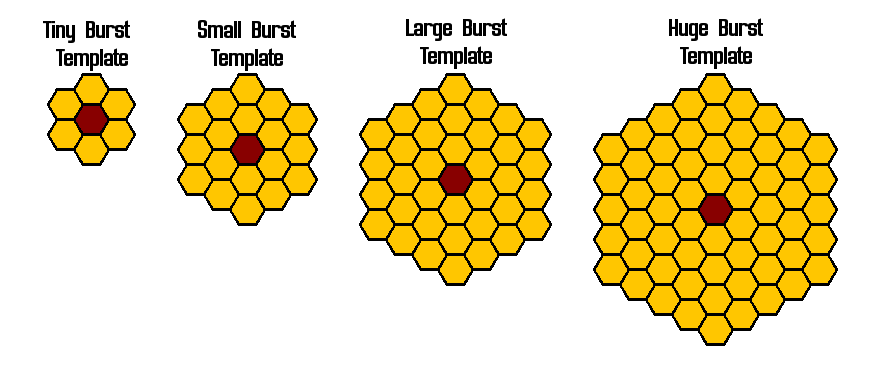
\includegraphics[width=14cm]{FoE_PnP_Burst_Templates_v2}
	\end{figure*}
	
	As suggested, \textbf{Area of Effect} (AoE) describes an area (hexes) where characters can be affected by certain effects. These effects include spells, enchantments, explosives, perk related auras, environmental hazards, traps and more.
	
	The AoE of explosives and spells are determined by the size of their burst, a radius of hexes. Explosive burst size may be changed with use of skills or perks. Burst size may not increase above Huge, but may be as small as one hex. Sizes are displayed on Picture 7.1.
	
	Enchantments depend on the Spirit Power of the spirit. Perk related auras have their AoE indicated within said effect. Environmental hazards have their AoE indicated by the GM, for instance an electrified floor for the entire room.
	
	
	\subsection*{Status Effects}
	\addcontentsline{toc}{subsection}{Status Effects}
	Status effects are various bonuses and penalties caused by attacks, weapons, chems and weather conditions. Their duration, effects and removal vary.
	
	Status effects that have a duration of up to 10 rounds and do not deal damage cease at the end of combat. Damage-dealing effects, like Burning and Bleeding, continue their effects normally unless immediately treated after combat.
	
	\begin{table*}[t]
		\centering
		\caption{Status Effects and Their Removal}
		\label{Table:7.5}
		\rowcolors{1}{gray!30}{gray!10}
		\begin{tabular}{|l|l|c|l|}
			\hline
			\textbf{Name}            & \textbf{Effect}                           & \textbf{Duration} & \textbf{Removal}                  \\
			Burning         & -2 HP / round                    &    3     & \begin{tabular}{@{}l@{}}Use all AP \& \\Drop prone \end{tabular} \\
			Bleeding        & -1 HP / round; Minor Distraction &    5     & First Aid Kit            \\
			Blinded         & -2 PER; -5 Combat skills         &    3     & -                        \\
			Crippled        & As per Crippled limb             & \begin{tabular}{@{}c@{}}Minor: 24h \\ Major: Removal \end{tabular}         & \begin{tabular}{@{}l@{}}Doctor's Bag, \\ Hydra\end{tabular}      \\
			Enraged         & \begin{tabular}{@{}l@{}}Berserk; +2 STR; \\ can only attack and move \end{tabular}                                 &    3     & Sedative                 \\
			Freezing        & +2 AP Cost of actions            &    5     & Alcohol                  \\
			Mind-Controlled & May act w/o her own volition     &    3     & Mind Bleach              \\
			Encumbered      & Cannot Sprint, Climb or Swim     & Until Removal         & \begin{tabular}{@{}l@{}}Remove excess \\ weight \end{tabular}                        \\
			Petrified       & Cannot act                       &    -     & \begin{tabular}{@{}l@{}}Failsafe,\\ Petrify-spell\end{tabular}  \\
			Stunned         & Cannot spend AP                  &    3     & Kickstarter              \\
			Unconscious     & Cannot act                       &    3     & Kickstarter              \\ \hline
		\end{tabular} 
		
		
	\end{table*}
	
	\subsubsection*{Burning}
	Character has caught on fire, either from attacks or the environment. They take damage every turn until the fire goes out, either by water, magic or other physical methods.
	
	\subsubsection*{Bleeding}
	Character has suffered considerable damage, bleeding from a gash for additional damage for five turns, unless the bleeding is stopped with applying Medicine, Bandages, Magic or other methods.
	
	\subsubsection*{Blinded}
	The character's vision has been hampered with in some way, such as by throwing sand into one's eyes or by magic. Though it doesn't have any clear ways to heal the condition, GM can give conditions for removal on a case-by-case basis, such as ``use 4 AP to remove the sand in your eyes''. The effect lasts for 3 turns.
	
	\subsubsection*{Crippled}
	Character has one or more of her limbs crippled, having taken either considerable or precise damage to them. Crippling can be Minor (a temporary state that heals naturally within a 24 hours.), Major (a near permanent state, that requires proper medical care of a doctor, or use of Magic, Chems or Doctor's Bag), or Severed (limb has been completely lost beyond recovery.) Crippled limbs affect the character in various ways. More information about being crippled can be found under this chapter, Combat Statistics - Crippled.
	
	\subsubsection*{Enraged}
	Character is filled with burning hatred, trying to smite anyone and anything that may have drawn their ire. While Enraged, the character is limited to Movement, Attack and Combat Trick actions, and may prefer melee combat over ranged. In addition, she doesn't care if her actions will have lethal risks in them. Sedatives are a quick yet risky solution to calm down a berserk character.
	
	\subsubsection*{Freezing}
	Character experiences chills and slowness in her numbing limbs, either from attacks or from the environment. Her actions are slowed, Actions cost +2 AP. Alcohol is a known, if fickle, cure.

	\subsubsection*{Mind-Controlled}
	The character is no longer truly themselves, unable to discern friend from foe - perhaps due to an invasive spell. There is a chance that the character attacks their closest ally rather than the intended enemy. Each time the Mind-Controlled character is about to attack, they must make a INT -2 roll to see if they hit an ally instead. On a failed roll, the ally is attacked instead. Mind Bleach is a costly, but effective cure for this state, as are certain medical spells.
	
	\subsubsection*{Encumbered}
	Character is carrying more that her maximum carry weight, or is burdened by heavy armor. She can stop being encumbered by either improving her carry weight with increases to her STR or by Perks, or by dropping the excess weight.
	
	\subsubsection*{Petrified}
	Character has turned into stone via magic, rendering them entirely unable to act. If this statue is smashed into pieces, the character dies. This nefarious magic can be countered with a Failsafe and Petrify spells.
	
	\subsubsection*{Stunned}
	Character has been stunned, often by a strong electric shock or heavy blunt blow. Her actions are limited to only perceiving and communicating with her surroundings. She is unable to act until her state of daze is over or someone helps her recover.
	
	Stun can be resisted with a successful END roll. If the character fails their roll, the character gains the Stunned condition as normal. If the roll is successful, and after the character has recovered from the stun, she is immune to another Stun attempt for 1 round.
	
	\subsubsection*{Unconscious}
	Character has suffered severe damage or has been knocked out by something. She is unable to act until she recovers consciousness or someone else helps her.
	
	
	\section*{Combat Actions}
	\addcontentsline{toc}{section}{Combat Actions}
	The most common combat actions are attacking and spellcasting. The AP costs for these actions depend on weapon or spell being used and are listed in the weapon's description on the Wasteland Wares. Actions taken with Telekinesis still require the normal AP costs to take. 
	
	Characters in combat will want to perform more complex and tactical actions than just attacking and spellcasting.  These are divided into Movement Actions, Attack Actions, Combat Tricks, Defensive Actions and Other Actions.  Below is a list of combat actions that a character may choose to take and their associated AP costs. No effect or combination of effects can reduce any action's AP cost below 1.
	
	
	\subsection*{Movement Actions}
	\addcontentsline{toc}{subsection}{Movement Actions}
	Movement actions allow a character to traverse a distance for part of their AP.  Conditions can impose a bonus or penalty to the character's movement. For example, moving through deep snow, crippled limbs and over-encumbrance can give a penalty.
	
	\subsubsection*{Ground Movement}
	Basic ground movement is \textbf{1 AP per 2 meters (1 hexes)} the character moves. Crippled wings do not interfere moving on ground.
	
	\subsubsection*{Flying}
	If a character is capable of flight, she may perform aerial movement, charging and sprinting actions.
	
	In combat, basic flight movement is \textbf{1 AP per 2 meters (1 hexes)} the character moves.
	
	If one of character's wings gains the \textbf{Crippled} condition, she is unable to fly, but can still glide with base movement speed. If both of character's wings are Crippled, she is unable to fly or glide. If the character is in midair when her both wings gain Crippled conditions, she is in \textbf{Freefall} and takes falling damage accordingly.
	
	Out of combat, flying characters can reach their full potential speed. However, it may take a little time to reach full speed.
	
	\subsubsection*{Swimming}
	Swimming movement is \textbf{2 AP per 2 meters (1 hex)} the character moves. A character cannot charge while swimming. A character cannot swim if she has two or more \textbf{Crippled} limbs.
	
	If the character is swimming when at least two of her limbs gain Crippled conditions, she sinks and is in risk of \textbf{Drowning}. Crippled wings do not interfere swimming.
	
	Diving follows Drowning rules for holding breath, found under Chapter 5: Game Rules - Environmental \& Other Hazards
	
	\subsubsection*{Climbing}
	Climbing costs \textbf{3 AP per 2 meters (1 hex)} the character moves. A character cannot charge while climbing. A character cannot climb if she has two or more \textbf{Crippled} limbs. The GGM may request a character to roll STR check.
	
	If the character is climbing when at least two of her limbs gain Crippled conditions, she loses grip and is in \textbf{Freefall} and takes falling damage accordingly. Crippled wings do not interfere climbing.
	
	\subsubsection*{Difficult Terrain}
	Difficult terrain adds an extra 1 AP cost for movement. Such terrains include deep snow, slippery surfaces, piles of bodies, steep climbs, turbulent waters, underground tunnels and strong winds. The GM may request a character to roll an appropriate SPECIAL check - for example AGI on slippery surfaces.
	
	\subsubsection*{Sprinting}
	When the character spends all of her APs to movement actions, she is considered \textbf{Sprinting}. The character gains additional AP equal to the character's END/2 to be used in further movement actions. No other actions besides free actions cannot be done while Sprinting. The GM may request a character to roll appropriate SPECIAL checks during Sprinting due hasty movements.
	
	\subsubsection*{Charging}
	If a character can move in a straight line to her target and moves at least 4 meters (2 hexes), she may initiate a \textbf{Charge}. Charging gives the character +10 bonus to one Unarmed or Melee attack made immediately at the end of the movement. The attack deals 2d10 extra damage. Any following attacks do not gain these bonuses.
	
	However, Charging makes a character an easier target for her foes. Until start of the character's next turn, all enemies gain +5 bonus to any attacks made against the charging character.
	
	Charging cannot be done in \textbf{Difficult Terrain}.
	
	\subsubsection*{Crouched}
	Moving while crouched costs 2 AP per 2 meters (1 hex) the character moves. Standing up from crouch or vice versa does not cost AP. The character cannot crouch while Flying.
	
	\subsubsection*{Drop Prone}
	A character can drop to the ground for free and is considered \textbf{Prone}. While flying, a character cannot drop prone without landing.
	
	\subsubsection*{Crawling}
	Crawling while prone costs 3 AP per 2 meters (1 hex) the character moves. The character cannot crawl while \textbf{Flying}.
	
	\subsubsection*{Stand Up}
	Standing up from \textbf{Prone} costs 4 AP. If all of the character's limbs are \textbf{Crippled}, she cannot Stand Up without assistance.
	
	\subsubsection*{Jumping}
	\textbf{Longjump from Standing} - A character can only cover a short distance if they jump from standing. If the character's STR is less than 5, she can jump 2 meters (1 hex). If her STR is at or greater than 5 but less than 10, she can jump 4 meters (2 hexes). If her STR is at 10 or greater, she can jump 6 meters (3 hexes). This jump costs 3 AP.
	
	\textbf{Running Start} - With a running start of at least 4 meters (2 hexes) of movement, a character can jump up to her STR in meters (STR/2 hexes). AP cost is 1+ distance covered as per \textbf{Ground Movement}.
	
	\begin{verse}
		\emph{\textbf{Example:} Emerald Glint first takes 6 meters of running start movement (3 AP) and then jumps another 4 meters (2 AP). This would cost her a total of 5 AP.}
	\end{verse}
	
	\textbf{Jumping directly Upwards} - If the character's STR is less than 5, she can jump 0,5 meters. If her STR is at or greater than 5 but less than 10, she can jump 1 meter. If her STR is at 10 or greater, she can jump 1,5 meters. This jump costs 3 AP.
	
	\subsubsection*{Withdraw}
	Sometimes situation gets too hot to handle and a tactical retreat is the best option available. With an additional cost of 4 AP on top of normal movement, a character can withdraw from melee combat range without provoking \textbf{Attacks of Opportunity}. A character can Sprint with the remaining AP she has available.
	
	
	\subsection*{Attack Actions}
	\addcontentsline{toc}{subsection}{Attack Actions}
	To attack an opponent, the character must make a Skill Roll using the appropriate skill for the weapon that the character is wielding. Attacks made without weapons and attacks made with non-explosive thrown weapons use the Unarmed Skill. This roll is usually heavily modified by Combat Variables. Modifiers can adjust the difficulty of a task beyond the normal limit of plus or minus 50, up to a maximum of the character's Critical Failure rate or a minimum of the character's Critical Success rate.
	
	Attacks are subject to modifiers called \textbf{Combat Variables}, found in this chapter under Combat Statistics.
	
	\subsubsection*{Melee / Unarmed Attack} 
	To initiate a Melee or Unarmed attack, the character must be standing next to the foe she wants to strike (or within reach of long melee weapons, such as spear).
	
	Unarmed attacks with bare hooves, horns, claws or similar natural weapons usually cost 3 AP. When wielding other weapons, the AP cost is determined by the weapon's statistics.
	
	\subsubsection*{Ranged Attack}
	Ranged attacks can be initiated from any distance up to the weapon's maximum range, usually long range (L).
	
	AP costs for ranged attacks are determined by the used weapon's statistics.
	
	\subsubsection*{Throwing Weapons and Explosives}
	Attacks made with thrown weapons and throwable explosives can be initiated from any distance up to weapon's maximum range, usually short range (S). Thrown weapons use Melee Skill.
	
	AP costs for thrown attacks are determined by the used weapon's statistics.
	
	\subsubsection*{Placed Explosives}
	Placed explosives are placed on the ground or other suitable surface and therefore have melee range.
	AP costs for placed explosives are determined by the used weapon's statistics.
	
	\begin{figure}[t]
		\centering
		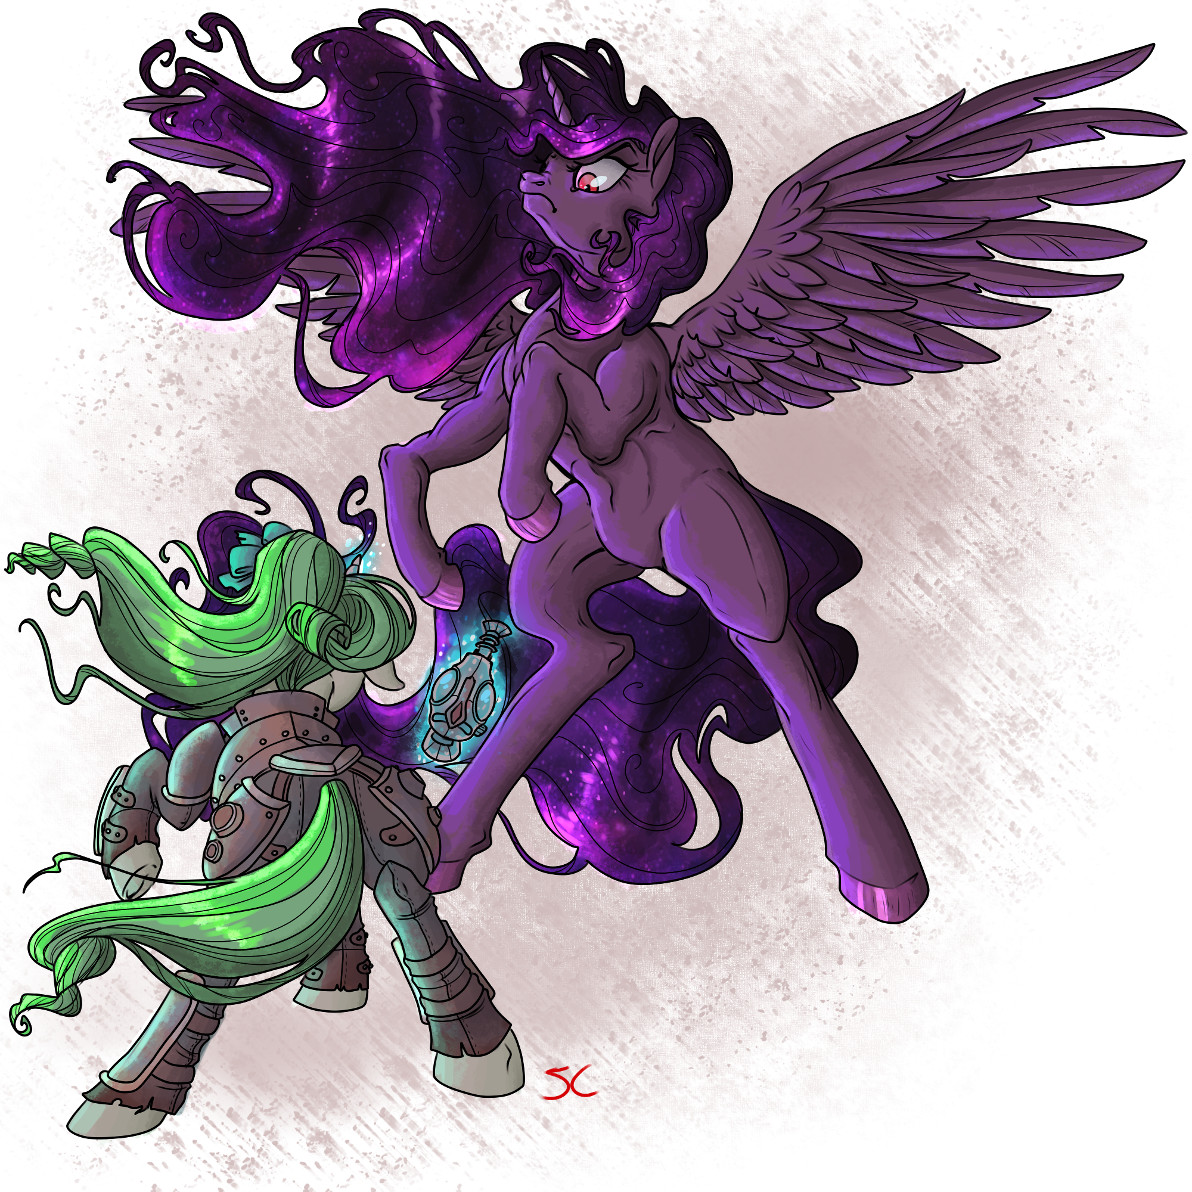
\includegraphics[width=0.8\linewidth]{ART/fight_1}
	\end{figure}
	
	\subsubsection*{Called Shot}
	When a character wishes to make a precise shot at her target, she performs a \textbf{Called Shot}, with additional 2 AP increase to her attack's AP cost. These attacks can hit a visible body parts, weak spots, and even disarm her targets. However, a Called Shot cannot be performed with weapons that have area or line of effect damage such as explosives and flame throwers.	

	Called shots are used to deal \textbf{Crippled} conditions to a target; it doesn't outright increase the damage dealt, but rather focuses the shot to break a particular limb exclusively. It should be noted that some enemies, such as most insects and robots have additional areas that are treated as limbs and can be Crippled.
	
	With each HP loss applied to the target during Called Shot, there is a cumulative 10\% chance to cripple the targeted limb. Some weapons have increased chance of inflicting Crippled, and this cumulative chance is applied on top of the Called Shot chance.
	
	Additionally, if the attack removes 2 or more HP through a Called Shot, the attacker can deal one less HP in damage and, in its place, guarantee a Crippled condition.
	
	Disarming weapons are considered Called Shots, and have their penalty listed below. A successful disarm deals 1 Condition Damage to the weapon (if Item Condition Rules are in effect) and forces the defender to roll STR. A success on the defender's part keeps the weapon in their control, but they must spend \textbf{Ready Weapon} action prior using the weapon again. A failure forces the defender to drop the weapon on an adjacent hex (up to GM which). 
	
	\begin{table}[t]
		\centering
		\caption{Called Shot Penalties by Limb}
		\label{Table:7.6}
		\rowcolors{1}{gray!30}{gray!10}
		\begin{tabular}{|l|l|l|}
			\hline
			\textbf{Target}                   & \textbf{Ranged} & \textbf{Melee} \\ \hline
			Torso                    & -10    & -5    \\
			Limb (in. tails)         & -20    & -10   \\
			Head                     & -30    & -15   \\
			Weapon                   & -20    & -20   \\ \hline
			Specific part (i.e. eye) & \multicolumn{2}{l|}{Additional -20}              \\ \hline
		\end{tabular} 
		
	\end{table}
	
	\subsubsection*{Aim}
	Character can increase her chance of success with an attack by performing an aim action. The action costs 2 extra AP to perform. This action increases the next attack's chance to succeed by 10. One can make only one aim action per attack action.
	
	The bonus to skill roll may be modified by weapon accessories and modifications.
	
	\subsubsection*{Reload}
	When a weapon runs out of ammunition, it must be reloaded according to the weapon's clip type. The types are listed under Chapter 3: Equipment - Weapon Characteristics.
	
	\subsubsection*{Casting a Spell}
	When a character wants to cast a spell in combat, she must make a Thaumaturgy roll. If the roll succeeds, she acts according to common spellcasting rules, found in Chapter 8: Magic \& Spells.
	
	AP and Strain costs for spells are determined by the used spell, and the values can be found in\emph{ \textbf{Magic Codex}}.
	
	Combat Variables may sometimes affect the casting of a spell. Check the skill modifiers provided in this chapter, under Combat Statistics - Combat Variables.
	
	\subsubsection*{Sneak Attack}
	After a successful \textbf{Sneaking} attempt, or when the target is otherwise unaware, one can perform a Sneak Attack. She gains a bonus of 15 to her chance to deal \textbf{Critical Damage} (doesn't affect actual skill hit chance). Character can make a Sneak Attack with any attack, except explosives. The \textbf{AP cost} for Sneak Attack is increased by 2 compared to the normal attack.
	
	After her Sneak Attack, the character may try a new \textbf{Use Skill (Sneak)} action with a penalty of -30. If the action is successful, she gets away unnoticed and may make another Sneak Attack. However, the attack itself is always noticed - with Melee or unarmed sneak attacks, only the victim notices the attack made against him, while ranged attacks are noticed by everyone who could either hear or see the attack.
	
	\vfill
	\begin{verse}
		\emph{\textbf{Example 1:} Featherfall wants to perform a sneak attack on a nasty raider. She successfully rolls for Sneak and catches the raider off-guard, moving in to backstab him. Her LCK is 5, so with a bonus of 15, her Critical Damage Threshold for the attack would become 20. She rolls for her Melee skill - which is 18 - and gets a result of 19. Despite the roll being under the Critical Damage Threshold, the attack is a failure because it is over her Skill level. The roll being within the Critical Damage Threshold does not guarantee an automatic success.}
	\end{verse}
	
	\begin{verse}
		\emph{\textbf{Example 2:} Featherfall has taken a vantage spot to snipe from with her hunting rifle - performing a sneak attack on a raider boss. She has succeeded in her Sneak Check, and her LCK is 5 so her Critical Damage Threshold for the attack would be 20. She rolls for Firearms skill - which she has at 70 - and gets a result of 12. The result is both under the Critical Damage Threshold and her Skill value, and thus Featherfall successfully hits and deals Critical Damage to the raider boss. If she had rolled over the Critical Damage Threshold, she had dealt normal damage.}
	\end{verse}
	
	\begin{verse}
		\textbf{Note:} Silenced weapons reduce the Use Skill (Sneak) action penalty by 15.
	\end{verse}
	
	\vfill		
	\subsubsection*{Attacks of Opportunity}
	Whenever a character performs an action that would cause a gap in her defense, nearby opponents in melee range may use this to their advantage. In other words, they gain \textbf{Attacks of Opportunity} (AoO), which are special melee or unarmed attacks. These are quick attacks that must be engaged immediately (on other characters' turns). A character may normally perform only 1 AoO per round, she must see the target and hold an appropriate weapon.
	
	Only melee or unarmed attacks with AP cost of 5 or less can be used to perform these attacks. This means that perks, special attacks or other effects that lower AP cost may allow the use of AoO with weapons that usually have too high AP cost. An AoO costs no AP.
	
	\bigskip\noindent
	The following activities provoke AoO from nearby opponents:
	\begin{compactitem}
		\item Leaving opponent's melee range (whether the character starts her turn in melee range or moves through melee range on her turn). If the character uses \textbf{Withdraw}, she does not provoke AoO.
		\item Accessing items not stored in the quick slots or weapon slots (backpack, saddle bags).
		\item Picking up objects.
		\item Interacting with environment, such as turning on the lights, using switches or valves.
		\item Using a placed explosive or mine, or disarming explosives.
		\item Using a skill that requires attention, i.e. Lockpick, Mechanics, Medicine (curing crippled limbs), Science (hacking), or Thaumaturgy
		\item Failing on \textbf{Start Grapple} action, using \textbf{Escape Grapple} and fleeing, or ending Grapple and fleeing.
	\end{compactitem}
	
	\bigskip	
	The GM may also declare AoO on other situations when the character's defense is hindered.
	
	\begin{verse}
		\emph{\textbf{Example:} Maabara is currently adjacent to a hostile raider, and she wishes to drink a health potion and run away from the enemy. She has none in her quick slots, so she has to access her inventory for one. By doing so, the raider - wielding a knife - gains an Attack of Opportunity on Maabara, though he misses. After downing the potion she runs away from the raider with her remaining AP without using Withdraw action. This would provoke an Attack of Opporunity for the raider, but as he already performed his one AoO already, Maabara can run away without fear of reprisal.}
	\end{verse}
	
	
	\subsection*{Combat Tricks}
	\addcontentsline{toc}{subsection}{Combat Tricks}
	\subsubsection*{Grapple}
	Grapple is the art of wrestling an opponent in a chaotic ball of flailing limbs. Size modifiers apply to all rolls in Grapple. It's not the best to wrestle with a full-grown dragon as a small filly.
	
	Grapple is between two characters, an attacker who initiated the grapple and defender who is grappled. Both STR and Unarmed can be used in Grapple-rolls unless otherwise specified.
	
	If at any point the defender rolls Critical Success for her opposed Unarmed or STR roll, she may leave the grapple.
	
	Allies can assist the grappling characters as per \textbf{Assist Ally} action.
	
	
	\bigskip\noindent
	\clearpage
	\textbf{\emph{Starting Grapple}}
	
	This action costs 5 AP.
	
	To initiate the grapple the character rolls an opposed roll against an adjacent target. If the attempt is successful, both characters gain the Grappled condition and can do the following Grapple actions on their turn. For the grapple to remain in effect, one character must Maintain it each round.
	
	\bigskip\noindent
	\textbf{\emph{Maintain Grapple}}
	
	This action costs 2 AP.
	
	To maintain the Grapple, the attacker must wish to continue the grapple and rolls an opposed roll against the defender. If the attacker wishes not to maintain the grapple, the grapple ends at the end of the current combat round.
	
	\bigskip\noindent
	\textbf{\emph{Overpower Grapple}}
	
	This action costs 4 AP.
	
	The defending character can try to turn the tide of the grapple by trying to overpower the attacker. The defending character rolls an opposed roll against the attacker.
	
	If successful, the defender becomes the attacker and vice versa. 
	
	\bigskip\noindent
	\textbf{\emph{Attack}}
	
	A character can deal damage with Unarmed weapons, One-Hoofed Melee Weapons or Pistols of any kind. This actions costs AP as listed in the used weapon's statistics and uses the weapon's skill to determine a success. However, the weapon used can cause a penalty to the roll as detailed below:
	
	\bigskip
	\begin{tabular}[h]{ll}
		Unarmed & no penalty \\ 
		Melee, One-Hoofed & Minor Distraction \\ 
		Pistols & Major Distraction \\ 
	\end{tabular} 
	
	\bigskip\noindent	
	\textbf{Pin}
	
	This action costs 8 AP for the first time, 4 AP for maintaining.
	
	The attacker rolls an opposed roll with a penalty of 30 against the defender to \textbf{Pin Down}. The defender rolls without penalty.
	
	If the attacker wants to hold his foe Pinned after the first round, she rolls an opposed roll against his target (without the penalty of 30) with an AP cost of 4 to maintain the pinning down.
	
	The Pinned character can try to use \textbf{Break Free} action on her turn, with her roll being an opposed roll against the attacker. If the pinned down character is successful in his or her roll or their Break Free action, they may stand up but is still considered to be Grappled.
	
	\bigskip\noindent
	\textbf{\emph{Tie Up}}
	
	This action costs 8 AP.
	
	When the defender has been \textbf{Pinned Down} successfully, the attacker pinning her down can try to tie her up in place of maintaining the pinning. Tying up requires one to have materials to bound one up such as chains, rope or wires.
	
	The attacker rolls an opposed roll with a penalty of 30 against his target to Tie Up. The defender rolls without penalty. After successful Tie Up no following Grapple actions are needed, and the grapple immediately ends.
	
	Tied up character can try to use \textbf{Break Free} action on her turn to break free of her bonds.

	\bigskip\noindent	
	\textbf{\emph{Move Grapple}}
	
	This action costs 4 AP.
	
	The attacker rolls an opposed roll against the defender, followed by a Move action to shift the grapple location with a cost of 3 AP / 2 meters (1 hex).
	
	Move Grapple action is only required once per combat turn to allow movement.
	
	\bigskip\noindent
	\textbf{\emph{Escape}}
	
	This action costs 4 AP.
	
	The defender can try to escape a grapple with an opposed roll against the attacker. Escaping the grapple can also be done with Break Free action.
	
	This action is an automatic success if the attacker doesn't wish to continue the grapple.
	
	\bigskip\noindent
	\textbf{\emph{Toss}}
	
	This action costs 8 AP.
	
	A character, either the attacker or the defender, can Toss their opponent with an opposed roll with a penalty of 30. The opponent rolls without penalty.
	
	On a success, the character can toss her opponent 2 meters (1 hex). She can with a successful STR check to toss her opponent an additional 2 meters (1 hex) to a total of 4 meters (2 hexes). The tossed opponent immediately gains Prone condition once landing on the new spot.
	
	If the opponent is successfully tossed, grapple immediately ends. On a fail, nothing happens and the grapple continues.
	
	\subsubsection*{Suppressive Fire}
	With full auto weapons (\textbf{F}) a character can provide Suppressive Fire to an area, possibly pinning enemies down.
	
	This action costs 8 AP and uses 20 units of appropriate ammo.
	
	The area affected by Suppressive Fire is a Large Burst Template centered within the weapon's effective range (up to Long). The area lasts until the character's next turn.
	
	The opponents under Suppressive Fire's area may Drop Prone for free or hide behind cover (if they're behind one already) to avoid the hail of lead. Those who aren't aware of the attack cannot freely Drop Prone. All characters, prone or not, suffer Minor Distraction penalty for being under heavy fire.
	
	The characters who stand or move in the Suppressive Fire's area without cover must roll LCK to avoid damage. On a failed LCK roll, a character suffers the base damage of the weapon - that is, without the dice.
	
	\begin{verse}
		\emph{\textbf{Note:} If the character does another Action after Suppressive Fire, like moving or firing weapon normally, the effects of Suppressive Fire end prematurely.}
	\end{verse}

	\subsubsection*{Trip}
	Instead of dealing damage, the character can try to trip an opponent to the ground. This action requires the foe to be next to you; when using ranged weapons such as rifles to trip, the character uses the weapon's stock to sweep the foe off their feet.
	
	This action costs 5 AP.
	
	The character uses Melee or Unarmed skill with a penalty of 15 to determine the success of the attempt. Ranged and Melee weapons use Melee skill for this action, all the others use Unarmed. On a success, the target of the Trip action falls Prone. If flying, the target drops to freefall if they fail an AGI check after successful hit.
	
	\subsubsection*{Distract}
	Distracting an opponent can give an edge in combat - such actions include but are not limited to tossing snowballs, taunt and impulsive contemporary dance routine. Distraction actions never deal damage directly and are meant to redirect the foe's attention or disrupt their actions. The targeted foes must see, hear or feel the character's distraction.
	
	This action costs 4 AP.
	
	First the player declares they are going to distract opponents and describes how they will do it. The player then rolls for success - GM determines the skill or SPECIAL to be rolled, i.e. taunting requires an Intimidation roll and dance requires CHA roll. If no other SPECIAL or Skill applies, LCK is rolled.
	
	On a success the foes suffer Minor Distraction penalty - the exact number of foes affected is determined by the GM. On a critical success or well-roleplayed description of the distraction the foes suffer Medium Distraction penalty. Regardless of success, the character has gained the foes' attention.
	
	By default, Distractions last for 2 rounds.
	
	
	\subsection*{Defensive actions}
	\addcontentsline{toc}{subsection}{Defensive actions}
	\subsubsection*{Dodge}
	AP cost of 1, one opponent suffers penalty of 5 to hit. This is cumulative. This action cannot be used if you cannot move freely. These include Grappled, Stunned and Prone conditions.
	
	The character must see the target she's willing to Dodge.
	
	A character cannot Dodge against Area of Effect (AoE) attacks, such as explosives and spells affecting an area.
	
	\subsubsection*{Break Free}
	If the character is held \textbf{Pinned Down}, in \textbf{Grapple}, \textbf{Tied Up}, held still via telekinesis or in some other way restrained, she may try to \textbf{Break Free}. This action can be described in-game as using brute strength, bucking, wiggling out of bonds or any creative solution the GM deems reasonable.
	
	Character breaking free makes a STR, AGI or LCK roll (in some cases an opposed roll), determined by GM. If the roll is successful, she is freed and can act normally. The AP cost is usually 8 AP, but the GM may change it if appropriate for the situation.
	
	\begin{verse}
		\emph{\textbf{Note:} There are some cases when Break Free is not allowed, such as being chained or pinned beneath a huge object. Such situations are always determined by the GM.}
	\end{verse}
	
	
	\subsection*{Other Actions}
	\addcontentsline{toc}{subsection}{Other Actions}
	\subsubsection*{Ready Item}
	Taking and readying an item from the inventory costs 8 AP.
	
	Readying an item from a \textbf{Quick Slot} costs 3 AP.
	
	Readying a concealed item costs an additional 2 AP.
	
	\subsubsection*{Ready / Change Weapon}
	Taking and readying a weapon from the inventory costs 8 AP.
	
	Readying a weapon from a \textbf{Weapon slot} or change to another weapon in Weapon slot costs 3 AP.
	
	Readying a concealed weapon costs an additional 2 AP.
	
	\subsubsection*{Use Item / Function}
	Using a held item (other than a weapon), weapon accessories, PipBuck or an item in the environment usually costs 2 AP. If the task is uncommonly time-consuming or hard, the GM may declare a different AP cost for the action.
	
	% Skill Cost table
	\begin{table*}[t]
		\centering
		\caption{Skill/SPECIAL AP Costs \& Modifiers in Combat}
		\label{Table:7.7}
		\rowcolors{1}{gray!30}{gray!10}
		\begin{tabular}{|c|c|c|c|c|}
			\hline
			& \textbf{Easy, no rush} & \textbf{Easy, rush} & \textbf{Hard, no rush} & \textbf{Hard, rush} \\ \hline
			\textbf{Cost}      &     4 AP      &    2 AP    &     10 AP     &    5 AP    \\
			\textbf{Roll Modifier} &       -       &    -15     &       -       &    -30     \\ \hline
		\end{tabular} 
	\end{table*}
	
	\subsubsection*{Drop Item}
	Dropping an item normally costs 0 AP. However, if a character carefully places down an item, the action costs 3 AP. The GM may declare a different AP cost for the action if appropriate.
	
	\subsubsection*{Pick Up Item}
	Picking an item up from the ground costs 6 AP.
	
	\subsubsection*{Assist Ally}
	Assisting ally consist of many kinds of actions, such as helping pull up an ally, catching her mid-fall, passing on a held item or other rather simple and quick actions. These actions cost 2 AP. The GM may declare a different AP cost for the action if appropriate.

	
	\subsubsection*{Use Skill / SPECIAL}
	
	Using other than combat skills (Explosives, Firearms, Magic Energy Weapons, Melee, Unarmed) during combat costs a differing amount of AP depending on the action's difficulty and if the action is rushed or not.
	
	Rushing an action makes it harder, but costs less AP. The GM determines the category of character's action. The base AP costs for Skill and SPECIAL uses are found Table 7.7.
	
	The GM may declare a different AP cost for the action if appropriate.
	
	NOTE: The GM may declare that some actions do not cost AP at all. For example, general PER rolls would cost no AP, but intense studying of environment or searching would cost AP.
		
	\subsubsection*{End Spell}
	Dropping a concentration of a spell or ending a spell with duration costs 0 AP.
	
	\subsubsection*{Talking}
	Short commands and sentences have no AP cost, but long speeches or monologues will have an AP cost as determined by Use Skill -action. After all, the enemies are hardly there to listen how you cite Shakespeare.
	
	
	\section*{Damage Calculations}
	\addcontentsline{toc}{section}{Damage Calculations}
	
	\subsection*{Damage \& Damage Threshold}
	\addcontentsline{toc}{subsection}{Damage \& Damage Threshold}
	When an attack skill roll is successful, the character usually deals damage. With weapons and explosives, the damage values are determined by the weapon's statistics. Damage consists of two or three parts: STR (melee/unarmed), base value and dice rolls.
	
	For example, with super sledge, the weapon's statistics indicate the damage as follows: $STR*2+40+(4)$. This means that the character's STR is doubled, added with the base value of 40, and finally rolling 4 dice. 
		
	Damage die is always d10, unless \textbf{Item Condition} additional rule is used in the campaign. Further information on Item Condition rules can be found under Chapter 3: Equipment - Optional Rules.
	
	\textbf{Damage Threshold} (DT) determines how much of the incoming damage is absorbed by the target's armor and other defenses. The leftover damage is then translated as lost HP tokens.
	
	\vfill
	
	\subsection*{Losing HP Tokens HP Tokens}
	\addcontentsline{toc}{subsection}{Losing HP Tokens HP Token}
	Characters do not take the weapon damage as is, but rather translate the incoming damage into lost HP tokens on their Character Sheet's \textbf{Health Tracker}. \emph{If the damage overcomes the target's DT, that automatically removes 1 HP token.}* Additionally target loses 1 HP token for every 10 points of damage over the DT value. A quick reference on total HP tokens lost based on damage received is displayed on Table 7.8.
	
	\begin{table}[!b]
		\centering
		\caption{Lost HP Token Thresholds}
		\label{Table:7.8}
		\rowcolors{1}{gray!30}{gray!10}
		\begin{tabular}{|l|c|}
			\textbf{DMG after DT} & \textbf{HP Lost} \\
			1-9*         & 1       \\
			10-19        & 2       \\
			20-29        & 3       \\
			30-39        & 4       \\
			40-49        & 5       \\
			50-59        & 6       \\
			60-69        & 7       \\
			70-79        & 8       \\
			80-89        & 9       \\
			90-99        & 10      \\ \hline
		\end{tabular} 		
	\end{table}

	\begin{table*}[t]
		\centering
		\caption{Pain Penalties}
		\label{Table:7.9}
		\rowcolors{1}{gray!30}{gray!10}
		\begin{tabular}{|l|l|l|}
			\hline
			\textbf{d10}  & \textbf{Penalty} & \textbf{Effect}                                       \\ \hline
			1-2  & Rattled & Minor Distraction                            \\
			3-4  & Bruised & Minor Distraction, +1 to AP Costs            \\
			5-6  & In Pain & Medium Distraction, +2 to AP Costs           \\
			7-8  & Maimed  & Random limb Crippled                         \\
			9-10 & Panic   & Cannot use Attack actions, unless no other way out \\ \hline
		\end{tabular} 
	\end{table*}

	\begin{verse}
		\emph{\textbf{Example:} Shining Example has been shot by a Raider, who has managed to do 65 damage to him. Shining Example's DT is 10. As the incoming damage is larger than Shining's DT, he automatically loses 1 HP. Next, the DT value of Shining is subtracted from the damage: 65-10 = 55. As 10 can fit in 55 five times (5*10 = 50, but 6*10 = 60), this means Shining loses 5 additional HP tokens. Overall, Shining Example has lost 6 HP, and must now subtract them from his Health Tracker.}
	\end{verse}

	
	\subsection*{Pain Thresholds}
	\addcontentsline{toc}{subsection}{Pain Thresholds}
	When a character's HP is lowered to the \textbf{Health Tracker's} lower end, special penalties come into effect to simulate one's body beginning to fail as it has sustained too much damage.
	
	Pain Thresholds come into effect at 5-4 HP, 3-2 HP and 1 HP. When a character ends up in these HP Tokens, GM rolls a 1d10 to deduce the penalty from table below. Once character's HP drops further, GM rolls for a new effect that replaces the earlier penalty.
	
	At 0 HP, the character is considered dead.
	
	
	\subsection*{Critical Damage \& Critical Damage Threshold}
	\addcontentsline{toc}{subsection}{Critical Damage \& Critical Damage Threshold}	
	When the character's attack skill roll is successful and within the critical damage threshold, she deals Critical Damage. Critical damage threshold is usually character's normal skill \textbf{critical success chance} but some factors, such as Sneak Attack and weapon modifications, may increase the threshold.
	
	For critical damage, the character rolls for damage normally, and then multiplies the result, usually by 2. Some weapons have greater critical multipliers than 2.
	
	\begin{verse}
		\emph{\textbf{Note:} Explosive weapons do not deal critical damage. If one performs a critical success with these weapons, other additional effects may occur.}
	\end{verse}

	
	\subsection*{SPECIAL Damage}
	\addcontentsline{toc}{subsection}{SPECIAL Damage}	
	Some attacks deal damage to character's SPECIAL attributes as well as to her HP. When a character receives SPECIAL damage, they put the amount of damage received into the character sheet's ``Temporary'' column on the SPECIAL section, on the respective SPECIAL stat currently taking damage.
	
	\begin{verse}
		\emph{\textbf{Example: }Doc Red's head has been crippled by a powerful blow, giving him SPECIAL damage to both his Perception and to his Intelligence. Doc Red's player puts a -4 on Perception and -2 on Intelligence to the Temporary column on the SPECIAL-section. This means that their respective stats are lower for a time being until his crippled head is healed.}
	\end{verse}
	
	
	\subsection*{Healing HP}
	\addcontentsline{toc}{subsection}{Healing HP}
	There are many ways of regaining HP tokens; the near-instant gratification of costly potions, visiting towns and cities' designated doctors or having a medical practitioner of your own. Of these three, only one saves you caps; having a practitioner of your own.
		
	\subsubsection*{Practicing Medicine}
	A learned wastelander can perform rudimentary medicine on the field, provided they have the tools. With First-aid kits and Doctor's Bags, the character can heal lost HP quickly and reliably.
	
	Without tools such as First-aid kit, a medical practitioner can attempt to boost the wounded character's natural healing rate to further assist the healing process, but cannot replenish HP outright. 
	
	Successful Medicine-check gives the wounded character +1 to their Healing Rate. Critical success gives +2 instead.
	
	Removing physical status effects such as bleeding can also be done without tools, but requires a successful Medicine-check. Fixing a Major Cripple requires a Doctor's Bag.
	
	\subsubsection*{Doctor Visit}
	Visiting a doctor, an NPC in a town is a guaranteed way to get a wounded character healed, as no checks aside from possible bartering of price is required. 
	
	However, doctors do not practice their craft for free; each healed HP token costs \textbf{20 caps}. This means that doctors can get expensive quickly, if great amount of HP is lost. This price can vary depending on location, the characters' barter skill or GM.
	
	In addition, doctors can remove Rad tokens, but the procedure is considerably more costly affair: \textbf{40 caps} per each Radiation token removed. This price can likewise be affected by various things. Doctors can also remove Major Cripple conditions, but that likewise costs money - \textbf{50 caps} per limb that needs to be sewn together.
	
	\begin{table}[b]
		\centering
		\caption{Doctor's Fees}
		\label{Table:7.10}
		\rowcolors{1}{gray!30}{gray!10}
		\begin{tabular}{|l|l|}
			\hline
			\textbf{Case}     & \textbf{Cost/Piece} \\ \hline
			Lost HP  & 20 Caps    \\
			Rads     & 40 Caps    \\
			Crippled & 50 Caps    \\ \hline
		\end{tabular} 
	\end{table}
	
	\subsubsection*{Using Potions}
	Potions are perhaps the least hassle one can have when healing their wounded. Usually costly but near-instant, they provide an easy way for even the dumbest of wastelander to remain healthy, provided they have Caps to spend. 
	
	Though not necessarily rare by any means, acquiring potions can be limited by traders' current stock or by sheer bad luck of not coming across any. A variety of potions can be found in the \emph{\textbf{Wasteland Wares}}.
	
	\chapter{Magic \& Spells}
	\noindent
	Magic and spells are both the mundane and the fantastical part of a pony's life, coming to some of them as easy as breathing, while others are clearly asthmatic. Nonetheless, magic is inherent in all of the races in their own ways. Some use magic for even the smallest of actions, while others carefully calculate the weight and effect of their spells.
	
	This chapter is meant to give rules and boundaries to all things magic. Spells for the various racial magic can be found in the \emph{\textbf{Magic Codex}}, an addition document for this rulebook.
	
	
	\section*{Spell Rules}
	\addcontentsline{toc}{section}{Spell Rules}
	All races are magical in their own way, capable of interacting with their surroundings and others with spells. Unicorns focus the magic on their horn, giving them a capability of manipulating the magic to make specific spells, while zebras can infuse natural brews with their magic, or call Spirits to aid them. Pegasi use their wings to pull off maneuvers, while Earth ponies' close ties to the earth give them strength and protection. In addition, there are special items that possess magical qualities. Even some monsters are capable of wielding magic.
	
	Below is a short reminder of the governing spell statistics (some perks and traits may alter how these statistics are determined):
	
	\begin{description}
		\item[Spirit Affinity] - determines the maximum power of summoned spirits.
		\item[Potency] - determines the power of spells. Potency is determined by the spell school of each individual spell. Generally speaking, the more Potency you have, the better.
		\item[Strain] - determines the amount of fatigue gained by casting the spell. The amount of Strain the character can withstand is static. Strain cost is determined by the spell. Strain recovers fully with rest.
	\end{description} 
	
	The exact descriptions of these statistics and how to determine them can be found in Chapter 2: Characters - Secondary Statistics.
	
	The exact descriptions of all spells, alchemical recipes and spirits can be found in \emph{\textbf{Magic Codex}}.
	
	% Magic Codex Image
	\begin{figure}[h]
		\centering
		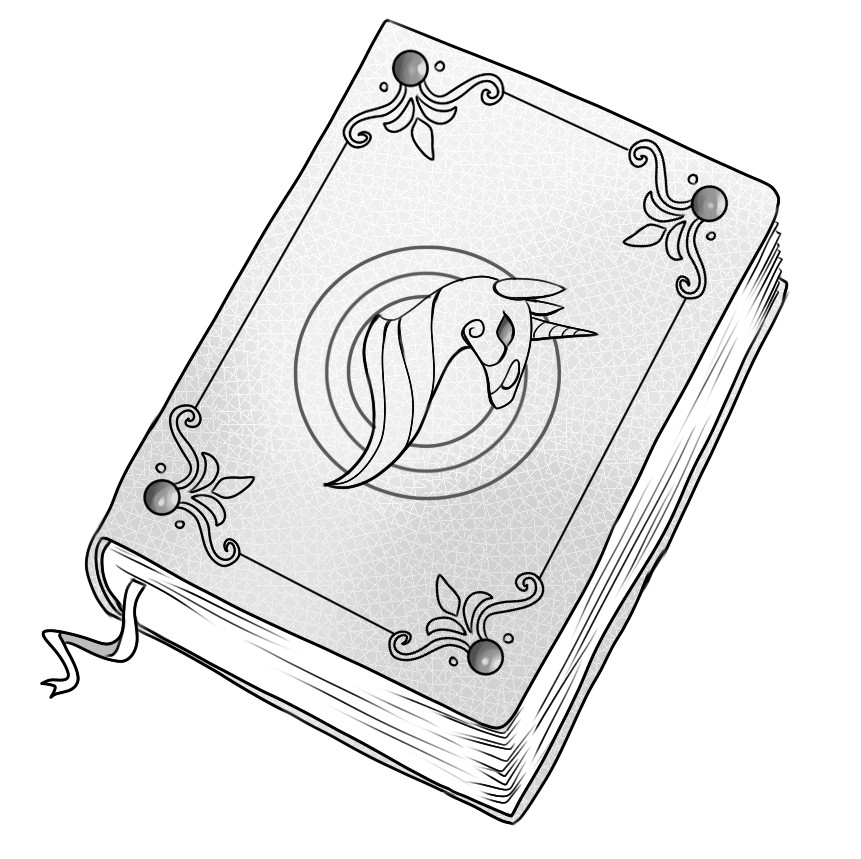
\includegraphics[width=0.7\linewidth]{ART/book}
	\end{figure}
		
	\clearpage
	
	
	\section*{Spell Characteristics}
	\addcontentsline{toc}{section}{Spell Characteristics}
	\subsection*{Magic School}
	Spells and maneuvers are divided into several different schools, representing alternate types of magic. Each school has a governing SPECIAL, matching the attribute that is the most important for that school, effectively determining \textbf{Potency} for all the spells or maneuvers in that school. Some characters are better at one line of magic than others, and vice versa.
	
	\subsection*{AP Cost \& Strain Cost}
	Using spells is much like attacking with weapons: the caster spends an \textbf{AP cost} as indicated by the spell and an effect occurs according to the description of said spell. After that, a certain amount of \textbf{Strain} affects the caster. If the caster is disturbed during the casting of her spell, she must roll \textbf{Thaumaturgy}-skill on her casting.
	
	Casting more than one spell in a turn is exhausting, increasing the Strain cost of the following spells. For the second spell after the first the cost is increased by 1, the third by 2, and so on.
	
	Should the casting fail, the character spends the AP as dictated by the Spell, but doesn't lose any Strain - she has spent time doing the required actions of the spell, but an error caused the spell to fail and thus not exhaust the character as greatly.
	
	If casting a spell would cause the caster to spend more Strain than she has, she can still cast the spell, but the excess Strain is taken as damage. The character loses 1 HP per point of excess Strain. This can kill the caster.
	
	\vfill
	
	\subsection*{Range}
	Each spell has a range. Unlike with weapons, spells have a maximum range and cannot be cast beyond that range. The range of each spell is explained in their description.
	
	\subsection*{Target \& Area}
	Some spells require a specific kind of target to function (ponies, creatures, objects, etc.) Some spells work on several targets, determined by either the number of targets or the targets within a certain range or area. Then there are spells that affect only the caster.
	
	There are spells that target an area with the target center within the spell's maximum range. Some spells affect the area around the caster.
	
	\subsection*{Duration \& Concentration}
	Some spells have durations and linger around for a while. The duration is noted in spell's description in either rounds or real time. If the caster wishes to do so, she can end the spell prematurely by using an \textbf{End Spell} action (costs 0 AP).
	
	Spells that require multiple turns to cast call for concentration from the caster. If the caster is interrupted during the casting, i.e. taking damage or suffering from Distraction, she has to roll Thaumaturgy to keep her concentration on the spell. This action requires no AP or Strain from the caster, as it is reactionary.
	
	Combat will always be considered difficult to a Spellcaster and a Thaumaturgy roll is required for all spells cast during combat or similar situations. Any Distraction modifiers affect a Thaumaturgy roll.
		
	\vfill
	
	\subsection*{Opposed rolls with Spells}
	Some spells allow the target to resist the spell with an opposed roll. Usually the caster rolls for the governing SPECIAL of the spell, and the target rolls the SPECIAL attribute determined by the spell.
	
	\begin{verse}
		\emph{\textbf{Example:} Emerald Glint casts Mirage on a chasing slaver to fool him into going to another direction. The Mirage spell dictates that the person whom the spell is casted on can oppose it with INT or CHA, whichever is higher against Emerald Glint's CHA. Emerald Glint's CHA is 7, the slaver's CHA is 6, meaning that their opposed rolls are 70 and 60 respectively. Emerald Glint rolls 56, while the Slaver rolls 40. This means Emerald Glint's Degree of Success is 14, against the Slaver's 20. Due to the Slaver having rolled better, he sees through the Mirage spell and continues pursuit.}
	\end{verse}
	
	\clearpage
	
	
	\section*{Earth Pony Magic}
	\addcontentsline{toc}{section}{Earth Pony Magic}
	Earth Pony Magic is its own special breed, channeled by the Earth Ponies from the soil and ground. Each Earth Pony has their own way of connecting, channeling and manipulating this breed of magic - it is highly intuitive, and teaching the ways of Earth Pony Magic is tedious and requires hard work.
	
	Earth Pony Magic is divided under three SPECIAL stats: STR, PER, and CHA. These provide venues for Earth Ponies to connect with the earth, and potentially each other. In order to successfully channel these energies, the Earth Pony character must succeed in a \textbf{Thaumaturgy} check.
	
	While spells based on STR of the character have been utilized in hard work around farms and wastes through the ages, PER and CHA based spells mainly developed to bring the community more tightly together. 
	
	\subsection*{Learning Spells}
	At the beginning of play, the Earth pony character may pick 2 spells. Earth ponies have no restrictions on what spells they can begin with.
	
	Unlike other ponies' arcane powers, the magic of Earth ponies is more of an intuitive process. This distinct difference means that Earth ponies may not learn new magical spells outside of leveling up.
	
	As mentioned, every 5 levels the character can learn a new spell of their choosing, which is immediately added to their arsenal. It is wise to consult the GM on spell choices.
	
	\vfill
	
	\subsection*{Earth Pony Spell List}
	Detailed spell list and description can be found in the appendix book \emph{\textbf{Magic Codex}} under Earth Pony Magic.
	
	\begin{description}
		\item \textbf{Strength Related Spells (STR)}
		\begin{compactitem}
			\item Adrenaline Rush
			\item Crash This Barn
			\item Enchanted Hooves
			\item Fortify
			\item Mend
			\item Overgrow
			\item Protection of the Earth
			\item Rooted
			\item Stone Shield
		\end{compactitem}
		\item \textbf{Perception Related Spells (PER)}
		\begin{compactitem}
			\item Earthly Warning
			\item Find Poison
			\item Improve Obstacle
			\item Smart Cookie's Invocation
		\end{compactitem}
		\item \textbf{Charisma Related Spells (CHA)}
		\begin{compactitem}
			\item Cheer
			\item Comforting Words
			\item Enhance Plant
			\item Healing Hooves
			\item Inner Circle
			\item Plant Caller
			\item Sound Mind
		\end{compactitem}		
	\end{description}

	\vfill
	
	\begin{figure*}[t]
		\centering
		\includegraphics[width=0.8\linewidth]{"ART/Chapter 8_Aerial Maneuver Wonderbolt edit"}
	\end{figure*}
		
	
	\section*{Pegasus \& Griffin Aerial Maneuvers}
	\addcontentsline{toc}{section}{Pegasus \& Griffin Aerial Maneuvers}
	Aerial Maneuvers are battle-tactics that utilize airborne stances and weather. Most commonly these are known to be used by pegasi and griffons, as they are notorious for this kind of combat.
	
	Aerial Maneuvers are categorized with different SPECIAL stats; AGI, END and CHA. This means that there is more than one way of one being a skilled aerial fighter. To pull off each maneuver, the flier must succeed in a \textbf{Thaumaturgy} check.
	
	The Maneuvers based in AGI and END were largely used as combat tactics in the Great War by pegasi and griffons alike, while CHA based Maneuvers are show-tricks turned to a more lethal purpose.
	
	Besides these three categories, a flier can invest in their flying speed instead of taking a maneuver upon level-up. Each time they improve their flight speed, they gain 2 meters/1 hex to their flight distance.
	
	\subsection*{Learning Maneuvers}	
	Pegasi start with 3 Maneuvers on first level while griffons start with 2.
	
	Pegasi learn a new Aerial Maneuver every 5th level (6, 11, 16) after first level and griffons learn a new Aerial Maneuver every 6th level (7, 13, 19) after first level.
	
	\textbf{Wonderbolt Maneuvers} and \textbf{Talon Maneuvers} require at least level 10 to be learned. After this, they can be learned as any other maneuvers, with Wonderbolt Maneuvers exclusive to pegasi and Talon Maneuvers exclusive to griffons. Difference to normal maneuvers is that the character twists these to fit their style, thus allowing them to use either AGI, END or CHA to determine their strength.
	
	In addition to this natural learning, the Aerial Maneuvers can be learned during gameplay either through a magazine, through a flight instructor and by self-taught training.
	
	In the Equestrian Wasteland one can sometimes find a copy of a flight magazine called \emph{``Aerodynamics Monthly''}. This magazine was published during the war to showcase the techniques used by Wonderbolts. Reading this magazine will teach 1 new Aerial Maneuver per magazine, and the specific Maneuver learned is decided by the player.
	
	To learn a new Maneuver by self-teaching, one must have a successful AGI/END/CHA -2 roll, depending on the Maneuver the character wants to learn. To learn a maneuver, the character must roll 4 successful checks, however, only one check may be made per day. The character may re-roll this check once per day.
	
	Having a teacher to coach the character reduces the required successful checks from 4 to 2.
	
	\subsection*{Aerial Maneuver List}
	Detailed maneuver list and descriptions can be found in the appendix book \emph{\textbf{Magic Codex}} under \emph{Aerial Maneuvers}.
	
	\begin{description}
		\item \textbf{Endurance-based Maneuvers (END)}
		\begin{compactitem}
			\item Defensive Spiral
			\item Dirt Drag
			\item Divebomb
			\item Plummet
			\item Sonic Rain-Nuke
			\item Twister
		\end{compactitem}
		\item \textbf{Charisma-based Maneuvers (CHA)}
		\begin{compactitem}
			\item Cloud Manipulation
			\item Defog Twirl
			\item Fantastic Flash
			\item Fire Trail
			\item Sun Celebration
			\item Tactical Weather Manipulation
		\end{compactitem}
		\item \textbf{Agility-based Maneuvers (AGI)}
		\begin{compactitem}
			\item Buccaneer Blaze
			\item Contrail
			\item Creeping Barrage
			\item Hightail Sweep
			\item Tornado
			\item Weave Defense
		\end{compactitem}
		\item \textbf{Talon Maneuvers (AGI/END/CHA)}
		\begin{compactitem}
			\item Blackwing's Mettle
			\item Carrion's Blight
			\item Gawd's Glorious Featherbedding
			\item Gilda's Feline Frenzium Furiatus
			\item Henrietta's Threatful Bravura
		\end{compactitem}
		\item \textbf{Wonderbolt Maneuvers (AGI/END/CHA)}
		\begin{compactitem}
			\item Commander Easyglide's Esprit de Corps
			\item Fleetfoot's Fix-it-up
			\item General Firefly's Double Inside-Out Loop
			\item Rainbow Dash's Sonic Rainboom
			\item Spitfire's Icarian Sun Salute
			\item Surprise's Sneak Sweep
		\end{compactitem}	
	\end{description}
	
	\begin{figure*}[t]
		\centering
		\includegraphics[width=0.9\linewidth]{"ART/Chapter 8_Unicorn magic"}
	\end{figure*}
	\vfill
	
	
	\section*{Unicorn Magic}
	\addcontentsline{toc}{section}{Unicorn Magic}
	Unicorn Magic, or as some say arcane magic, is easily the most versatile and studied magic found in the Wasteland. If there is a unicorn around, one can bet arcane spells to appear eventually. 
	
	Arcane spells are divided into \textbf{Magic Schools}, each with their primary, governing SPECIAL stat that determines the spell's \textbf{Potency} and strength. Exceptions to this are \emph{General Magic} and \emph{Metamagic} schools, where the unicorn can choose any SPECIAL stat they want on the former, and either CHA or INT stat on the latter.
	
	Each magic school is geared towards a certain use. For example, Conjuration Magic revolves around creating something with or from one's magic, while Illusion Magic attempts to fool or distract others.
	
	\subsection*{Learning Spells}
	At the beginning of play, Unicorns pick 3 spells alongside \emph{Light} and \emph{Telekinesis} spells, unless she has picked \textbf{One Trick Pony} -trait. Usually one can pick any spell, but sometimes one must choose a particular school, from which all of her spells must be drawn.
	
	An exception to this is \textbf{Dark Magic school}, which is a collection of particularly vile and heinous spells. Not to mention that they're rare, and as such picking spells from the school will be under GM discretion.
	
	Characters can learn new spells in two ways - through leveling up or seeking out and experimenting on their own. As mentioned, every 5 levels the character can learn a new spell of their choosing, which is immediately added to their arsenal. It is best to consult the GM on spell choices. 
	
	To learn a new spell by self-teaching, one must make \textbf{4 successful} SPECIAL -2 rolls, depending on the school of the spell. However only one check may be made per day, and the character may re-roll this check once per day.
	
	Having a teacher to coach the character reduces the required successful checks from 4 to 2.
	
	\subsection*{Unicorn Spell List}
	Detailed spell list and description can be found in the appendix book \emph{\textbf{Magic Codex}} under Unicorn Magic.
	
	\begin{description}
		\item \textbf{General Magic (pick one SPECIAL)}
		\begin{compactitem}
			\item Arcane Mark
			\item Light
			\item Telekinesis
			\item Teleport
		\end{compactitem}
		\item \textbf{Conjuration Magic (INT)}
		\begin{compactitem}
			\item Arcane Blast
			\item Bend Surface
			\item Call Object
			\item Eldricht Knives
			\item Pocket Sand
			\item Shield
			\item Storm Cloud
			\item Wall of Energy
		\end{compactitem}
		\item \textbf{Dark Magic (END)} \emph{(Picking spells from this school is always under GM discretion)}
		\begin{compactitem}
			\item Blood Weapons
			\item Devouring Darkness
			\item Fear
			\item Heart Attack
			\item Life Surge
			\item Shadow Form
			\item Soul Jar
			\item Vile Crystals
		\end{compactitem}
		\item \textbf{Enchantment Magic (CHA)}
		\begin{compactitem}
			\item Bypass
			\item Compulsion
			\item Discord
			\item Magic Trance
			\item Resilience
			\item Soft Light
			\item Standstill
			\item Want It, Need It
		\end{compactitem}
		\item \textbf{Illusion Magic (CHA)}
		\begin{compactitem}
			\item Invisibility
			\item Magical Fireworks
			\item Mirage
			\item Sensory Foil
			\item Silver Shroud
			\item Simulacrum
			\item Target
			\item Thrown Voice
		\end{compactitem}
		\item \textbf{Medical Magic (INT)}
		\begin{compactitem}
			\item Anesthetic
			\item Bone Mending
			\item Calm Mind
			\item Clean
			\item Enhancement
			\item Panacea
			\item Regeneration
			\item Restoration
		\end{compactitem}
		\item \textbf{Metamagic (CHA/INT)}
		\begin{compactitem}
			\item \#1 Assistant
			\item Bonds of Friendship
			\item Hidden Aura
			\item Power of Friendship
		\end{compactitem}
		\item \textbf{Perception Magic (PER)}
		\begin{compactitem}
			\item Amplify
			\item Combat Pre-Cognition
			\item Detection
			\item Magic Mirror
			\item Memory Manipulation
			\item Mind Probe
			\item Spy Connections
			\item Telepathy
		\end{compactitem}
		\item \textbf{Protective Magic (END)}
		\begin{compactitem}
			\item Alarm
			\item Cloak of Elements
			\item Equestria's Love
			\item Failsafe
			\item Friendly Critter's Help
			\item Mental Bulwark
			\item Rad-Guard
			\item Toughen Hide
		\end{compactitem}
		\item \textbf{Transmutation Magic (END)}
		\begin{compactitem}
			\item Come to Life
			\item Growth
			\item Petrify
			\item Phase
			\item Remake
			\item Shape Magic
			\item Steady Walk
			\item Transformation
		\end{compactitem} 
	\end{description}

	
	\section*{Zebra Magic}
	\addcontentsline{toc}{section}{Zebra Magic}
	
	\subsection*{Alchemy}
	\addcontentsline{toc}{subsection}{Alchemy}
	Though to untrained eye the zebra alchemy looks like simple cooking of ingredients, the process is a bit more complicated than it seems. Zebra alchemists infuse their innate magic into their brews, thus bringing out the effects of the potions.
	
	Without this use of magic, the potion created would be little more than boiled leaf water. This is also the reason why these recipes are often so difficult to replicate by non-zebras.
	
	The zebras use various herbs, categorized as \textbf{Green, Red and Blue herbs}, and various mutant parts in their brews. Of the three herb types, Green are most common and Blue the rarest. Monster parts can be varied, such as Yao Guai blood, Abomination flesh pieces among others. Some recipes can also include other items such as syringes for containing the alchemical brew.
	
	\subsubsection*{Recipes}
	Zebra Alchemists start with 4 known recipes, which have a Skill Requirement of 30 or less. Alchemists can have self-made poisons, see Brewing Poisons, as starting recipes as long as the poison's Skill Requirement is 30 or lower.
	
	Memorizing new recipes varies a bit from unicorn's way of learning spells; the zebra way is more experimental, much like cooking something out of a whim and hoping it would turn out okay. The alchemist must have the Skill requirement and a single batch of ingredients required to make the potion she wishes to learn in-game.
	
	To learn a new recipe, she requires 4 \textbf{successful} Survival -20 checks. However, she can only make one learning check per day, and they are allowed to re-roll this check once per day.
	
	Having a physical recipe or a tutor for a potion lowers the required checks from 4 to 2.
	
	\begin{verse}
		\emph{\textbf{Example:} Maabara wants to learn how to make a Greater Healing Potion. She has the required 60 Survival and enough ingredients. She has no recipe, or a tutor to help her, so she must make 4 Survival -20 checks.}
	\end{verse}	
	
	\subsubsection*{Gathering Ingredients}
	Zebra Alchemists make potions out of the ingredients they find in the wild, from sprouting herbs to acquired body parts of various creatures.
	
	To find and gather herbs, the character must make a successful Survival check. A Penalty may be applied to the skill if the GM feels the place would usually be devoid of vegetation, making the herbs harder to find. When looting a downed creature, alchemists likewise roll Survival to gather the body part.
	
	\subsubsection*{Making a Brew}
	If the alchemist has the right listed ingredients and sufficient skill required - which may vary from the standard Survival -, she can make the recipe she desires.
	The alchemist rolls their required skill to see if the brew was successful. If the roll fails, the brew fails. If the brew is a failure, the alchemist has burnt their resources and must produce new ones to try again.
	
	Brewing normally takes a full hour for the alchemical mix to finish infusing, after which the potion is ready for use. On a critical success, the alchemical brew is made in half the time. In addition, each brewing attempt, be it successful or not, costs 2 Strain.
		
	\subsubsection*{Brewing Poisons}
	An alchemist can also craft poisons of their own or improve existing poisons, with certain ingredients causing different effects in the finished product. Each type of herb or special ingredient has a different effect and the quantity of the ingredient means for a larger, more serious effect. How these ingredients affect the end result is listed in Table 8.1.
	
	An alchemist spends one Green Herb to create a basic poison, with 1x40\% chance of poisoning. More details on poison can be found under Chapter 5: Game Rules - Environmental \& Other Hazards.
	
	Each ingredient type increases the requirement for the Survival check to craft the poison, with Green Herbs giving the least increase in the skill requirement and with mutant parts giving the most. However, this skill requirement increase will not go over 100.
	
	With mutant parts, the requirement increase is the same no matter what kind of part it is, though the player can and should discuss if the specific part would give a specific result, such as Ghoul horn giving additional damage to Unicorns or Irradiated Material giving radiation damage.
	
	\begin{figure*}[t]
		\centering
		\includegraphics[width=0.9\linewidth]{"ART/Chapter 8_Alchemy zeeb"}
	\end{figure*}

	\begin{table}[h]
		\centering
		\caption{Ingredients \& Their Use in Alchemy}
		\label{Table:8.1}
		\rowcolors{1}{gray!30}{gray!10}
		\begin{tabular}{|l|l|l|}
			\hline
			Ingredient  & Effect       & \begin{tabular}{@{}l@{}}Skill Req. \\ Increase\end{tabular} \\ \hline
			Green Herb  & Duration +1  & +10                 \\
			Red Herb    & \begin{tabular}{@{}l@{}}SPECIAL -1 / \\ HP -1 \end{tabular}             & +20                 \\
			Blue Herb   & \begin{tabular}{@{}l@{}}+1 Roll / \\ +10\% Chance \end{tabular}             & +30                 \\
			Mutant Part & Extra effect & +40                 \\ \hline
		\end{tabular} 
	\end{table}
	
	\begin{description}
		\item[Green Herb:] The most common herb, a single Green herb gives 1 turn added to the poison's duration. Each Green herb also gives +10 to Skill Requirement to craft the poison.
		\item[Red Herb:]  A moderately difficult herb to find, a single Red herb gives -1 SPECIAL damage or hurts the target with -1 HP in the poison's effect. Each Red herb added also gives +20 each to Skill Requirement to craft the poison.
		\item[Blue Herb:] The rarest of the herbs, a single Blue herb gives the poison a damaging effect, with each single Blue Herb giving an additional Poison roll or +10\% to the possibility of the poison having successfully made contact with the body. Each Blue herb added also gives +30 to Skill Requirement.
		\item[Mutant Part:] A body part or bodily fluids of a mutant creature, a single part added to the brew will give the poison an additional unique effect. What this effect is should be discussed with the GM. Adding a mutant part in the brew also adds a +40 to the Skill Requirement of the poison.
	\end{description}
	
	\begin{verse}
		\emph{\textbf{Example:} Maabara is brewing a poison of her own making. She chooses to use Green herb x1, a Red herb x1 to make the poison cause -1 to PER. In addition to this, she adds Blue herb x2 to give the base roll +1 and an extra +10\% to probability to succeed. This makes the Poison give the target -1 to PER for 1 Round, at 2x50\% chance of success.}
	\end{verse}
	
	
	\clearpage
	
	\subsection*{Shamanism}
	\addcontentsline{toc}{subsection}{Shamanism}
	A shaman is a powerful magic wielder that relies on spirits for results. Spirit magic takes form as either enchantments on items or through direct magic (much like spells). These can be achieved by either bartering with spirits or by binding spirits. Zebras are the masters of shamanism, although not nearly all zebras are capable of this kind of magic.
	
	\subsubsection*{Spirit Affinity}
	Shamans possess a unique secondary stat called \textbf{Spirit Affinity}, which is somewhat similar to unicorns' Potency. It indicates how powerful spirits the shaman can summon, barter with and bind. Spirit Affinity is solved with the following formula:
	
	\begin{center}
		$lvl+CHA$
	\end{center}
	
	The exact use of Spirit Affinity varies depending on which kind of spiritual interaction takes place, and sometimes it even varies depending on the type of spirit in question. These are explained in the appropriate sections.
	
	\subsubsection*{Spirit Power}
	Different spirits have different strengths. \textbf{Spirit Power} indicates the power of the spirit, as well as the power of magic it uses. The more powerful the spirit is, the harder it is to summon, barter with or bind. However, the stronger the spirit is the greater the spirit magic effects are.
	
	Spirit Power rating is a number between 1 and 15 (usually between 1 and 10). The exact effect of Spirit Power varies and are explained in future sections or in the details of each individual spirit.
	
	\subsubsection*{Interacting with Spirits}
	Shaman knows the world of spirits, and the spirits know and hear the shaman's call. At the beginning of the summoning ritual, the shaman chooses her end goal - will she try to imprison the spirit in a \textbf{Spirit Prison} or strike a deal with the spirit and store its power in a \textbf{Rune}.
	
	\begin{table*}[!t]
		\centering
		\caption{Spirit Summoning chart}
		\label{Table:8.2}
		\rowcolors{1}{gray!30}{gray!10}
		\begin{tabular}{|l|l|l|l|l|l|}
			\hline
			\begin{tabular}{@{}l@{}}\textbf{Spirit} \\\textbf{Power}\end{tabular} & \begin{tabular}{@{}l@{}}\textbf{Min. Spirit} \\ \textbf{Affinity} \end{tabular} & \begin{tabular}{@{}l@{}}\textbf{Bind} \\ \textbf{Resistance}\end{tabular} & \textbf{Barter} & \begin{tabular}{@{}l@{}}\textbf{Hostility} \\ \textbf{Chance} \end{tabular} & \textbf{HP} \\ \hline
			1            & 2                    & 5               & 20     & 2\%              & 4  \\
			2            & 4                    & 10              & 25     & 4\%              & 6  \\
			3            & 6                    & 15              & 30     & 6\%              & 8  \\
			4            & 8                    & 20              & 35     & 8\%              & 10 \\
			5            & 10                   & 25              & 40     & 10\%             & 12 \\
			6            & 12                   & 30              & 45     & 12\%             & 14 \\
			7            & 14                   & 35              & 50     & 14\%             & 16 \\
			8            & 16                   & 40              & 55     & 16\%             & 18 \\
			9            & 18                   & 45              & 60     & 18\%             & 20 \\
			10           & 20                   & 50              & 65     & 20\%             & 22 \\
			11           & 22                   & 55              & 70     & 30\%             & 26 \\
			12           & 24                   & 60              & 75     & 40\%             & 30 \\
			13           & 26                   & 65              & 80     & 50\%             & 34 \\
			14           & 28                   & 70              & 85     & 60\%             & 38 \\
			15           & 30                   & 75              & 90     & 70\%             & 42 \\ \hline
		\end{tabular} 
		
	\end{table*}

	\begin{figure*}[t]
		\centering
		\includegraphics[width=0.8\linewidth]{"ART/Chapter 8_shamanism"}
	\end{figure*}	
	
	Summoning spirits requires a great deal of focusing and effort. This means that should a shaman try to summon a spirit in combat, she has to invest AP to Use Skill action, with any combat penalties that apply with it. She can summon spirits in other kinds of tough situations too, although she receives a penalty to her summoning roll depending on the level of distraction.
	
	Prisons and Runes can be used to deliver the spirit's magic in form of a spell, or as enchantments on items. The exact effects of each spirit are explained in \emph{\textbf{Magic Codex}}, under Zebra Magic - Spirit Magic.
	
	Table 8.2 indicates the required Spirit Affinity for the summoning process, as well as the spirit's power, Barter and Hostility chance.
	
	\vfill
	
	\bigskip\noindent
	\textbf{Spirit Binding in a Prison}
	
	Binding a spirit means the shaman forcefully subjugates the spirit into a \textbf{Spirit Prison}. This allows the shaman to use spiritual magic without bartering with the spirit. In addition, the shaman doesn't have to spend the effort of summoning the spirit when she needs the magic.
	
	Spirit Prisons are vessels capable of containing a spirit, keeping them locked in. Spirit Prisons are simple one-use containers, such as gems or flasks, which can be crafted using \textbf{Thaumaturgy} skill.
	
	Crafting Spirit Prisons isn't particularly hard. One must simply obtain a suitable base for the item (for example, a vial or a gem worth at least 100 caps), and then spend 10 minutes crafting the container and rolling for her Thaumaturgy skill.
	
	The result of the roll determines the strength of the container: for every 5 points under the skill threshold, the container can hold 1 point of Spirit Power. A critical success on the roll results the created Spirit Prison to be able to hold any spirit regardless of Spirit Power.
	
	To capture a spirit, one must succeed in a Thaumaturgy roll, with a penalty equal to the spirit's Bind Resistance value. If the shaman succeeds, the spirit is helplessly captured within the container. If not, the process fails and the spirit may turn hostile as per its Hostility. If it doesn't attack the shaman, it flees but remembers the attempt, possibly returning later for revenge.
	
	The maximum number of active Spirit Prisons a shaman can have at any time is equal to half of her Spirit Affinity. If a spirit is bound and the shaman already has the maximum number of active Spirit Prisons, the spirit in the oldest prison will break free. If the Spirit Prison is damaged and/or broken, the spirit may escape, remove enchantments it has granted, and even attack the shaman. Only one spirit may be contained in a vessel at any time.
	
	\begin{verse}
		\emph{\textbf{Example:} Maabara crafts a Spirit Prison using a crystal vial worth 100 caps. Her Thaumaturgy skill is 40 and she makes a successful roll. The result is 25, a total of 15 under her skill value. This means that the maximum Spirit Power the vessel can contain is 3 (15 / 5 = 3).}
	\end{verse}
	
	\bigskip\noindent
	\textbf{Spiritual Favors with Runes}
	
	The shaman can negotiate with the spirit about granting the shaman a favor or two, as opposed to the more violent and forceful act of using a Spirit Prison. The shaman must possess something worth value to the spirit, as it wouldn't be bargaining if she didn't have anything to give in return.
	
	The magic of spirits is stored within a \textbf{Rune}, a spiritual item that allows the spirit magic to interact with the material world. Runes can be crafted by shaman using gems or other items that spirits would value. Usually they bear the symbol of the spirit which power it holds. Empty Runes can be created by shamans and can hold the magic of one spirit at a time. The creation takes 10 minutes without any roll required, but costs 10 \textbf{Strain} from the shaman.
	
	Upon summoning the spirit peacefully, the shaman offers her deal to the spirit. The bargaining is an opposed roll, where the shaman rolls their Barter skill against spirit's Barter. The spirit may offer a favor worth its Spirit Power, but the shaman may ask for less. For every 1 Spirit Power less the shaman asks for, she gains a bonus of 5 to her Barter roll (maximum bonus of 30).
	
	Spirits value emotional value and effort more than material value. This means that the spiritual gifts are not necessarily expensive items. Nonetheless, these are used as a form of currency. The gift may provide a bonus or a penalty to the shaman's Barter roll. This is determined by the GM.
	
	If the bartering is successful, the spirit lends some of its power to shaman. If the bartering result is a tie, and the spirit's Spirit Power is 10 or less, the shaman wins. Otherwise the spirit wins, and flees contently without providing any power. If the shaman critically fails her Barter roll, the spirit becomes hostile and attacks the shaman.
	
	The maximum number of active Runes (as enchantments or spell reserves) is equal to half of shaman's Spirit Affinity.
	
	\subsubsection*{Spirit Combat}
	Sometimes the spirit turns hostile. This may be be the result of an unskilled shaman Sometimes the spirit turns hostile. This may be the result of an unskilled shaman summoning it or failing miserably in bartering, or the spirit is simply unfriendly to begin with. Whatever the case, an unfriendly or annoyed spirit may attack the shaman and her friends. When a Spirit turns hostile, they also become more tangible in order to cause damage to the subject of their ire.
	
	Due to them becoming tangible, Spirits take damage from weapons as would any mortal creature. When attacking, Spirits roll their Barter to confirm a hit. In addition to having their spells, as listed in the Magic Codex, Spirits can strike with a basic attack which deals damage with the following formula:
	
	\begin{center}
		$10+[Spirit \, \, Power * d10]$
	\end{center}
	
	The basic attack uses 5 AP. Unless otherwise specified, the basic attack is a melee attack and must be done into adjacent hex. In addition, spirits can have additional effects in their Basic attack, based on what kind of a spirit they are; Fire spirits' Basic attack is purely fire-damage, and can cause a Burning- status effect.
	
	Spirits have 20 AP at their disposal.
	
	Once their HP reaches 0, the spirit is stunned for 5 rounds. During this time the spirit is vulnerable to being captured or pacified. \textbf{The shaman can at this point either imprison the spirit in a Prison with a Thaumaturgy roll without penalties, or strike a deal with the spirit with a bonus of 30 to her Barter.} If neither option is made, the spirit vanishes after breaking the stun. Usually spirits that are bound or bartered with this way are not pleased with this and may return later for revenge.
	
	\bigskip\noindent
	\textbf{Pacifying a Spirit}
	
	If the shaman encounters a hostile spirit and a spirit combat begins, there is an option to soothe the spirit and end the combat peacefully.
	
	Shaman may spend 10 AP to try and negotiate with the spirit, making a Diplomacy check with a penalty equal to the spirit's Bind Resistance. If the shaman succeeds, the spirit calms down and becomes receptive to further bargaining. Upon failure, the spirit stays hostile.
	
	Shamans and characters with \textbf{Spiritually Awakened} trait can pacify a spirit, for the simple fact that only they truly understand the Spirit. One character can try to pacify a spirit only once per combat.
	
	\subsubsection*{Enchantments and Spells}
	After shaman has managed to either bind or successfully bargain with the spirit, she can use the spirit's magic. This can take shape in two different ways: \textbf{enchantments} and \textbf{spells}. If the spirit is bound within a Spirit Prison, there is no limit what the shaman may do. However, bargains may limit shaman's possible actions when she uses Runes.
	
	\bigskip\noindent
	\textbf{Enchantments}
	
	Enchantments are permanent (or semi-permanent) magical effects that enhance items. Usually they are used with armor and weapons, but occasionally with other items. Each Spirit Prison or Rune may grant only one enchantment, using the maximum Spirit Power. Once created, enchantments cannot be removed from the item using other than magic.
	
	Different spirits grant different enchantments. All enchantments are listed in \emph{\textbf{Magic Codex}}, under Zebra Magic - Spirit Magic.
	
	Enchanting an item is simple. One only needs a source of spirit magic and a target item. She must then spend 1 minute per Spirit Power to enchant the item. She must work undisturbed the whole duration. The Spirit Prison or Rune becomes an integral part of the item and grants its magical properties to the item - it cannot be used for spells after that.
	
	Permanent enchantments are always on effect. These include damage enchantments for weapons and damage resistance enchantments for armor.
	
	Semi-permanent enchantments work much like permanent enchantments but have limited number of uses. For example, armor may save the wearer from death once per day and up to 10 times. Once these kinds of enchantments have spent all of their uses, the enchantment disappears and must be reapplied.
	
	\textbf{When using a Spirit Prison}, the enchantment cannot be broken by the spirit. However, if the enchanted item takes damage directly, or is targeted by a dispelling effect such as Failsafe, the Spirit Prison may break (shaman rolls LCK). The enchantment immediately vanishes if the Prison breaks.
	
	\textbf{When using a Rune}, the enchantment works for as long as the shaman has the spirit's approval. If the spirit is displeased, it may break the bargain and the enchantment becomes obsolete. Shaman may regain the spirit's favor later, but until then the item in question is unenchanted.
	
	\bigskip\noindent
	\textbf{Spells}
	
	Each spirit type can cast certain spells. Usually spirits can cast all of the listed spells, but sometimes (for example, as a result of a bargain) they choose to cast only one or two different spells, even if they could cast any of them. All spells are listed in \emph{\textbf{Magic Codex}}, under Zebra Magic - Spirit Magic.
	
	In effect, casting a spell using spirit magic is similar to unicorn magic. There is a key difference, though. Unicorns have Strain that limits their casting, while shamans do not. Instead, her Spirit Affinity determines the total number of spells she may cast from a Spirit Prison or Rune.
	
	\textbf{If the shaman uses a Spirit Prison}, she has no maximum number of spells she may cast with it, and can use \textbf{Thaumaturgy} skill for checks. Instead, if she casts more spells than her \emph{[Spirit Affinity]/3} per day with a Spirit Prison, there is a solid 25\% chance that the Spirit Prison breaks. If this happens, the imprisoned spirit escapes and may attack the shaman or simply flee. This limitation affects each Spirit Prison individually.
	
	\textbf{If the shaman uses a Rune}, she may cast a number of spells equal to her [Spirit Affinity]/2 using the particular Rune, and can use \textbf{Barter} skill for checks. After these spells the Rune loses its charge. During the bargaining she may ask for more spells than this, but for each additional spell the shaman suffers a penalty of 5 to her Bartering skill.
	
	
	
	
	\chapter*{Glossary}
	\addcontentsline{toc}{chapter}{Glossary}
	The following are widely used terms in this document or within roleplaying games in general.
	
	\begin{description}
		\item[Action] - A thing Character does, usually for a price of Action Points (AP)
		\item[Bonus]  -  A positive effect on a roll determined by Game Master.
		\item[Caps] - The cold hard cash and currency of the Wastes; bottlecaps, Caps for short.
		\item[Character] - Any thinking creature in the game, including Player-controlled.
		\item[Character Sheet] - A sheet with information about your character and their stats.
		\item[Check]  -  Player rolling a dice and comparing the result to a value on their character sheet as requested by the Game Master.
		\item[Combat]  -  An event during which characters have to battle against opponents. Either by violence or by a combat of words.
		\item[Conflict] - see Combat.
		\item[Creature] - Anything that might be hostile to the player characters.
		\item[Dice]  - Shortened (x)D(y), dice are rolled to determine success or failing during play. For example, 2d6 means that 2 six-sided dice are rolled.
		\item[Experience Points (XP)]  -  Points given by the Game Master to the players to advance their characters.
		\item[Game Master (GM)]  -  The host of the game, enforcer of the rules and supplier of the story.
		\item[Ghoul]  - A pony, zebra or griffon mutated by the magical radiation. Resembles a walking corpse. Some stay sane while others go feral and hostile to others.
		\item[Group] - see Party.
		\item[Hex]  -  A single tile on a battle map, if one is used in the game.
		\item[House Rule]  - A rule made by the Game Master outside of this rulebook.
		\item[Initiative]  - The roll that determines the order in which characters act in combat.
		\item[Non-Player Character (NPC)]  - A character controlled by the Game Master.
		\item[Optional Rule]  - A rule that is not necessary for playing, but can be included for extra depth.
		\item[Party]  - The players' characters are collectively called a party.
		\item[Penalty]  -  A negative effect on a roll determined by the Game Master.
		\item[Perk]  -  A set of good qualities your character can take upon leveling up.
		\item[Player]  -  You and your fellow friends who will be playing.
		\item[Player Character (PC)]  - A character controlled by a player.
		\item[Race]  -  The species of your character, each of which have their own pros and cons.
		\item[Rads]  -  Magical radiation that is harmful to living creatures, causing potentially dangerous mutations.
		\item[Rolling] - The act of rolling the dice to see the effects of your actions.
		\item[Rounding] -  Unless otherwise specified in the rules or by the Game Master, all equations are rounded down to the nearest integer (full number).
		\item[Routine] - A mundane, everyday task a character performs, i.e. eating or sleeping. They are often not checked daily for their tedious nature of checking - instead only asked for in intense moments.
		\item[Secondary Statistics] - Character's statistics that are derived from some other statistic(s).
		\item[Session] - A period when the GM hosts the game for the players.
		\item[Spell] -  Magical spells that can be cast by the characters.
		\item[Stack] - Some abilities, perks and other effects may stack, meaning a bonus or a penalty is added on top of another one.
		\item[Terminal] - The computers of this world, somewhat primitive in technology.
		\item[Trait] -  An optional character-building quality that the player can pick for their character during character creation. Has both a pro and con to them, unlike perks.
		\item[Token] - A picture or a figurine representing your character. Optional. 
	\end{description}

	
	\onecolumn
	
	\chapter*{Combat Quick Reference Sheet}
	\addcontentsline{toc}{chapter}{Combat Quick Reference Sheet}
	{
	\rowcolors{1}{gray!30}{gray!10}
	\begin{longtabu} to 140mm{| X[l,2] | X[l,2]| X[l,3] | X[l,6] |}
		
		\hline
        \cellcolor{gray!50}     & \textbf{Name}           & \textbf{AP Cost}                  & \textbf{Notes}                                                                        \\ \hline
		\cellcolor{gray!50} Turn Order     & Initiative              & -                                 & 1d10+AGI Equal Initiatives compare PER, Equal PERs compare LCK. Highest goes first    \\ \hline
        \cellcolor{gray!50} Movement      & Ground Movement         & 1 AP per 2m / 1 hex               &                                                                                       \\
        \cellcolor{gray!50}      & Flying                  & 1 AP per 2m / 1 hex               & Crippled wings prevent flying                                                         \\
        \cellcolor{gray!50}      & Swimming                & 2 AP per 2m / 1 hex               & Cannot charge, cannot swim if 2 or more limbs Crippled                                \\
        \cellcolor{gray!50}      & Climbing                & 3 AP per 2m / 1 hex               & Cannot charge, cannot climb if 2 or more limbs Crippled                               \\
        \cellcolor{gray!50}      & Difficult Terrain       & +1 AP to Movement                 & May require SPECIAL roll                                                              \\
        \cellcolor{gray!50}      & Sprinting               & All AP to Movement                & Gain additional END/2 number of AP to Movement                                        \\
        \cellcolor{gray!50}      & Charging                & -                                 & +10 to melee/unarmed immediately after, additional 2d0 DMG. Opponents gain +5 to hit  \\
        \cellcolor{gray!50}      & Crawling                & 2 AP per 2m / 1 hex               & Cannot do while flying                                                                \\
        \cellcolor{gray!50}      & Drop Prone              & -                                 & Considered Prone after                                                                \\
        \cellcolor{gray!50}      & Crawling                & 3 AP per 2m / 1 hex               & Cannot do while flying                                                                \\
        \cellcolor{gray!50}      & Standing Up             & 4 AP                              & When Crippled, needs assistance                                                       \\
        \cellcolor{gray!50}      & Jumping, Still Longjump & 3 AP                              & STR <5, 2 meters/1 hex  STR 5-9, 4 meters/2 hex  STR 10, 6 meters/3 hex               \\
        \cellcolor{gray!50}      & Jumping, Running Start  & 2 AP                              & 4 meters/2 hex of movement required, can jump STR in meters (STR/2 hex)               \\
        \cellcolor{gray!50} \multirow{-13}{1,3cm}{}     & Jumping, Up             & 3 AP                              & STR <5, 0,5 meters    STR 5-9, 1 meter      STR 10, 1,5 meters                        \\
		\cellcolor{gray!50} Movement     & Withdraw                & 4 AP                              & Does not provoke AoO, may Sprint                                                      \\ \hline
        \cellcolor{gray!50} Attack Actions     & Attack                  & Weapon-specific                   & 1d100 result under or equal to Combat Skill results in a hit                          \\
        \cellcolor{gray!50}      & Called Shot             & +2 AP                             & Cripple body parts                                                                    \\
        \cellcolor{gray!50}      & Aim                     & +2 AP                             & +10 to combat skill for next attack                                                   \\
        \cellcolor{gray!50}      & Reload                  & Weapon-specific                   &                                                                                       \\
        \cellcolor{gray!50}      & Casting a Spell         & Spell-specific                    &                                                                                       \\
        \cellcolor{gray!50}      & Sneak Attack            & +2 AP                             & +15 to perform a Critical Hit                                                         \\
		\cellcolor{gray!50}      & Attack of Opportunity   & -                                 & Max 5 AP cost for melee or unarmed.                                                   \\ \hline
        \cellcolor{gray!50} Combat Tricks     & Grapple, Start          & 5 AP                              & Opposed Unarmed / STR                                                                 \\
        \cellcolor{gray!50}      & Grapple, Maintain       & 2 AP                              & Opposed Unarmed / STR                                                                 \\
        \cellcolor{gray!50}      & Grapple, Overpower      & 4 AP                              & Opposed Unarmed / STR                                                                 \\
        \cellcolor{gray!50}      & Grapple, Attack         & Weapon-specific                   & Unarmed: no penalty      Melee, 1-H: Minor Distraction      Pistol: Major Distraction \\
        \cellcolor{gray!50}      & Grapple, Pin            & 8 AP initiate, 4 AP maintain      & Opposed Unarmed / STR (Attacker -30)                                                  \\
        \cellcolor{gray!50}      & Grapple, Tie Up         & 8 AP                              & Opposed Unarmed / STR (Attacker -30); Grapple ends                                    \\
        \cellcolor{gray!50}      & Grapple, Move           & 4 AP + Movement                   & Opposed Unarmed / STR; Movement 3 AP per 2 m / 1 hex                                  \\
        \cellcolor{gray!50}      & Grapple, Escape         & 4 AP                              & Opposed Unarmed / STR                                                                 \\
        \cellcolor{gray!50}      & Grapple, Toss           & 8 AP                              & Opposed Unarmed / STR (Attacker -30); Grapple ends                                    \\
        \cellcolor{gray!50}      & Suppressive Fire        & 8 AP                              &                                                                                       \\
        \cellcolor{gray!50}      & Trip                    & 5 AP                              & Melee / Unarmed (-15); On success target is Prone                                     \\ 
		\cellcolor{gray!50}      & Distract                & 4 AP                              &                                                                                       \\ \hline
        \cellcolor{gray!50}  Defensive    & Dodge                   & From 1 AP to Maximum AP           & Cannot be used if no movement allowed; -5 per use against one opponent                \\ 
		\cellcolor{gray!50}      & Break Free              & 8 AP                              & STR / AGI, LCK if GM allows                                                           \\ \hline
    \cellcolor{gray!50} Other Actions        & Ready Item              & 8 AP from inventory; 3 AP from QS & +2 AP cost if concealed item                                                          \\
    \cellcolor{gray!50} Other Actions         & Ready / Change Weapon   & 8 AP from inventory; 3 AP from WS & +2 AP cost if concealed item                                                          \\
     \cellcolor{gray!50}         & Use Item / Function     & 2 AP                              & GM may change AP cost if extremely long time to use or similar                        \\
    \cellcolor{gray!50}          & Drop Item               & -                                 & If carefully dropped, costs 3 AP                                                      \\
    \cellcolor{gray!50}          & Pick Up Item            & 6 AP                              &                                                                                       \\
    \cellcolor{gray!50}          & Assist Ally             & 2 AP                              & GM may change AP cost depending on situation                                          \\
    \cellcolor{gray!50}          & Use Skill / SPECIAL     & Easy, no rush: 4 Easy, rushed: 2 	Hard, no rush: 10 
    
    Hard, rushed: 5	  & If rushed, -15 to Skill or SPECIAL roll; double penalty for Hard                      \\
    \cellcolor{gray!50}          & Maintain Spell          & Spell-specific                    &                                                                                       \\
    \cellcolor{gray!50}          & End Spell               & -                                 &                                                                                       \\
	\cellcolor{gray!50}          & Talking                 & -                                 & If used to influence others, check Use Skill                                          \\ \hline
	\end{longtabu}
	} 
	
	{
		\rowcolors{1}{gray!30}{gray!10}
		\begin{longtabu} to 140mm{| X[l,2] | X[l,6] |}
			\hline
			\textbf{Combat Variable} & \textbf{Modifiers}                                                                                                         \\ \hline
			Range                    & Point Blank 0; Short 0; Medium -10; Long -20                                                                               \\
			Visibility               & Normal 0; Twilight / Rain -5; Fog / Snowfall -10; Night / Heavy Fog -15; Dark Indoors / Dust Storm -20; Total Darkness -40 \\
			Distraction              & Minor -10; Medium -20; Major -30                                                                                           \\
			Cover                    & None 0; Partial -10; Great -30                                                                                             \\
			STR Requirement          & +1 AP cost, -5 for each STR value under requirement                                                                        \\
			Size                     & See Table 2.1                                                                                                              \\
			Braced Weapon            & STR Requirement -2; Range Medium 0; Range Long -10                                                                         \\
			Ranged in Melee          & Shooter gains Minor Distraction                                                                                            \\
			Prone                    & Gain Partial Cover against ranged; Cannot Dodge; -30 Melee / Unarmed                                                       \\
			Gang Up                  & +10 to Melee / Unarmed if adjacent to same target with an ally                                                             \\
			Grappled                 & Cannot access inventory; Move only with Move Grapple action                                                                \\
			Pinned Down              & Cannot use Movement actions; Major Distraction to actions sans Break Free                                                  \\
			Tied up                  & Cannot use Movement actions; Major Distraction to actions sans Break Free \\ \hline
		\end{longtabu}
	}

	{
		\rowcolors{1}{gray!30}{gray!10}
		\begin{tabular}{|l|c|}
			\textbf{DMG after DT} & \textbf{HP Lost} \\
			1-9*         & 1       \\
			10-19        & 2       \\
			20-29        & 3       \\
			30-39        & 4       \\
			40-49        & 5       \\
			50-59        & 6       \\
			60-69        & 7       \\
			70-79        & 8       \\
			80-89        & 9       \\
			90-99        & 10      \\ \hline
		\end{tabular} 		
	}
	
	\bigskip
	{
		\rowcolors{1}{gray!30}{gray!10}
		\begin{tabular}{|l|l|c|l|}
			\hline
			\textbf{Status}            & \textbf{Effect}                           & \textbf{Duration} & \textbf{Removal}                  \\
			Burning         & -2 HP / round                    &    3     & \begin{tabular}{@{}l@{}}Use all AP \& \\Drop prone \end{tabular} \\
			Bleeding        & -1 HP / round; Minor Distraction &    5     & First Aid Kit            \\
			Blinded         & -2 PER; -5 Combat skills         &    3     & -                        \\
			Crippled        & As per Crippled limb             & \begin{tabular}{@{}c@{}}Minor: 24h \\ Major: Removal \end{tabular}         & \begin{tabular}{@{}l@{}}Doctor's Bag, \\ Hydra\end{tabular}      \\
			Enraged         & \begin{tabular}{@{}l@{}}Berserk; +2 STR; \\ can only attack and move \end{tabular}                                 &    3     & Sedative                 \\
			Freezing        & +2 AP Cost of actions            &    5     & Alcohol                  \\
			Mind-Controlled & May act w/o her own volition     &    3     & Mind Bleach              \\
			Encumbered      & Cannot Sprint, Climb or Swim     & Until Removal         & \begin{tabular}{@{}l@{}}Remove excess \\ weight \end{tabular}                        \\
			Petrified       & Cannot act                       &    -     & \begin{tabular}{@{}l@{}}Failsafe,\\ Petrify-spell\end{tabular}  \\
			Stunned         & Cannot spend AP                  &    3     & Kickstarter              \\
			Unconscious     & Cannot act                       &    3     & Kickstarter              \\ \hline
		\end{tabular} 
	}
	
	\begin{figure}[!b]
		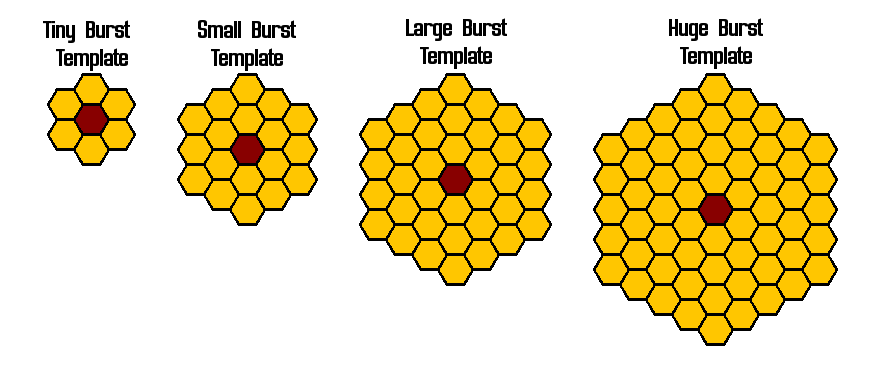
\includegraphics[width=14cm]{FoE_PnP_Burst_Templates_v2}
	\end{figure}

	\begin{figure*}[t]
		\centering
		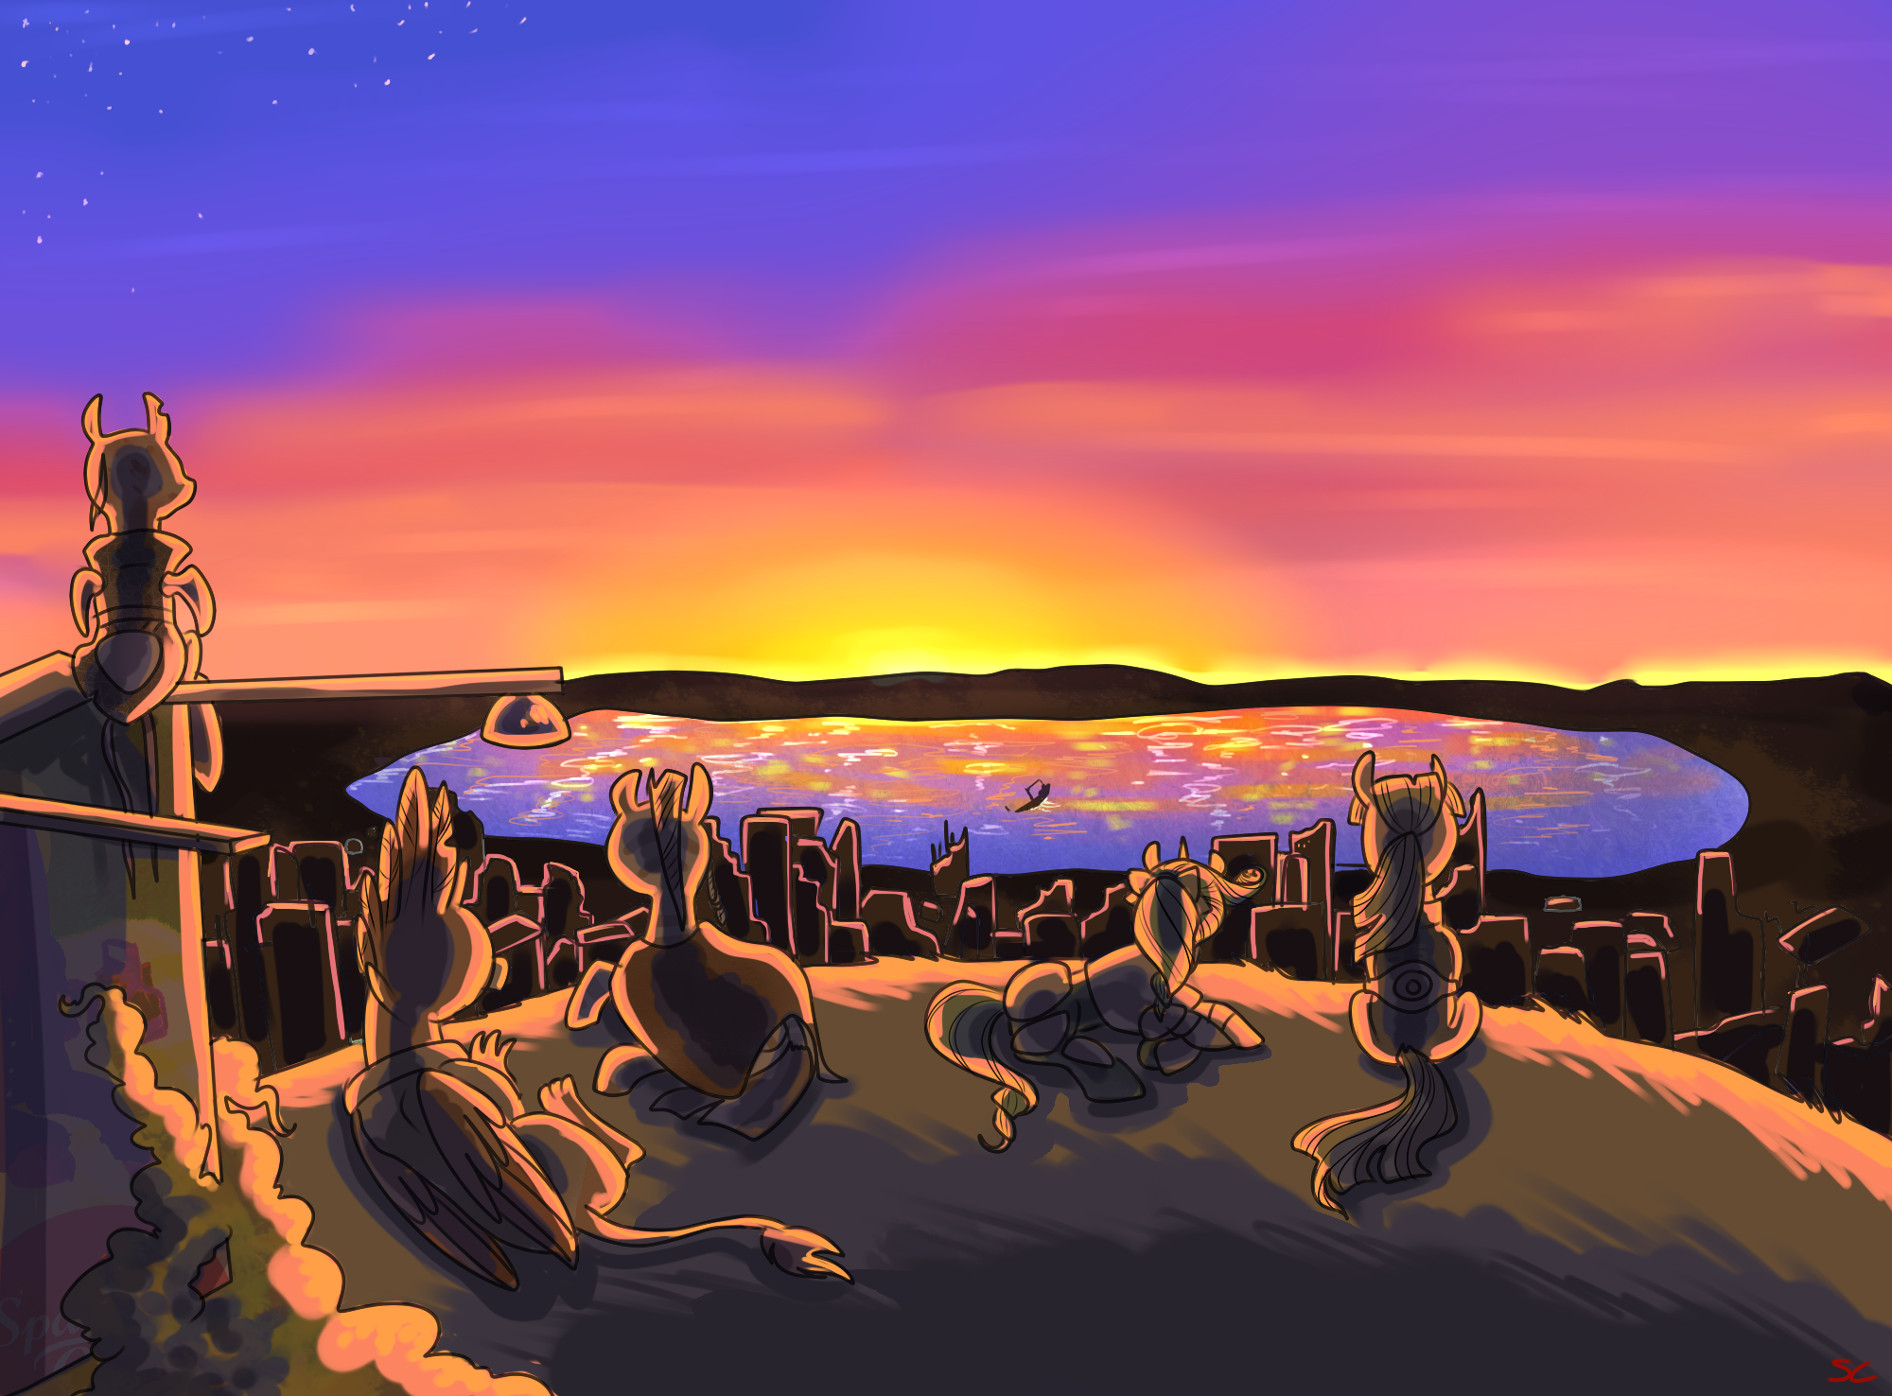
\includegraphics[width=1.1\textwidth]{ART/Sunrise}
	\end{figure*}
	
\end{document}